%=======================================================================
%  Chapter 3.  FURTHER PRELIMINARIES, WITH APPLICATIONS TO THE ANALYSIS
%              OF DEFORMATION
%  A from-scratch, motivated account of Steigmann & Shirani,
%  "Principles of Continuum Mechanics", Chapter 3, matching the book's
%  section and equation numbering.  Every step is shown, using only the
%  algebra of Chapters 1 and 2.  All nine chapter problems are solved.
%
%  Compile:  latexmk -pdf continuum_ch3.tex
%=======================================================================
\documentclass[17pt,a4paper]{extreport}

\usepackage[margin=1.8cm]{geometry}
\usepackage{amsmath,amssymb,amsthm}
\usepackage{bm}
\usepackage{accents}
% book style: boldface is rendered by an under-tilde
\DeclareRobustCommand{\vek}[1]{\underaccent{\tilde}{#1}}
\usepackage{xcolor}
\usepackage{enumitem}
\usepackage{graphicx}
\usepackage{tikz}
\usetikzlibrary{arrows.meta,calc,positioning,angles,quotes,patterns}
\tikzset{vec/.style={-{Stealth[length=2.3mm]},thick},
         thinvec/.style={-{Stealth[length=1.8mm]},semithick},
         mapar/.style={-{Stealth[length=2.4mm]},thick},
         guide/.style={gray!65,densely dashed,thin},
         lbl/.style={fill=white,inner sep=1pt}}
\newcommand{\blob}[1]{\draw[#1] plot[smooth cycle,tension=0.85] coordinates
  {(0,1.05) (1.15,0.72) (1.5,-0.35) (0.6,-1.15) (-0.75,-0.95) (-1.3,0.05)};}
\usepackage[colorlinks=true,linkcolor=blue!55!black,citecolor=blue!55!black,
            hypertexnames=false,pdfencoding=unicode]{hyperref}

%=============================== notation ==============================
\newcommand{\Rn}{\mathbb{R}}
\newcommand{\Cn}{\mathbb{C}}
\newcommand{\Et}{\mathcal{E}^{3}}
\newcommand{\hEt}{\hat{\mathcal{E}}^{3}}
\newcommand{\Vt}{\mathbb{E}^{3}}
\newcommand{\hVt}{\hat{\mathbb{E}}^{3}}
\newcommand{\Lin}{\operatorname{Lin}}
\newcommand{\Orth}{\operatorname{Orth}}
\newcommand{\Sym}{\operatorname{sym}}
\newcommand{\Skw}{\operatorname{skw}}
\newcommand{\tr}{\operatorname{tr}}
\newcommand{\grad}{\operatorname{grad}}
\newcommand{\Grad}{\operatorname{Grad}}
\newcommand{\dvg}{\operatorname{div}}
\newcommand{\Dvg}{\operatorname{Div}}
\newcommand{\I}{\vek{I}}
\newcommand{\hI}{\hat{\vek{I}}}
\newcommand{\Ob}{\vek{O}}
\newcommand{\hOb}{\hat{\vek{O}}}
\newcommand{\ba}{\vek{a}}
\newcommand{\bb}{\vek{b}}
\newcommand{\bc}{\vek{c}}
\newcommand{\bd}{\vek{d}}
\renewcommand{\bm}{\vek{m}}
\newcommand{\bn}{\vek{n}}
\newcommand{\bp}{\vek{p}}
\newcommand{\br}{\vek{r}}
\newcommand{\bs}{\vek{s}}
\newcommand{\bt}{\vek{t}}
\newcommand{\bu}{\vek{u}}
\newcommand{\bv}{\vek{v}}
\newcommand{\bw}{\vek{w}}
\newcommand{\bx}{\vek{x}}
\newcommand{\by}{\vek{y}}
\newcommand{\bz}{\vek{z}}
\newcommand{\bM}{\vek{M}}
\newcommand{\bN}{\vek{N}}
\newcommand{\bX}{\vek{X}}
\newcommand{\bY}{\vek{Y}}
\newcommand{\bZ}{\vek{Z}}
\newcommand{\bA}{\vek{A}}
\newcommand{\bB}{\vek{B}}
\newcommand{\bC}{\vek{C}}
\newcommand{\bD}{\vek{D}}
\newcommand{\bE}{\vek{E}}
\newcommand{\bF}{\vek{F}}
\newcommand{\bG}{\vek{G}}
\newcommand{\bH}{\vek{H}}
\newcommand{\bK}{\vek{K}}
\newcommand{\bL}{\vek{L}}
\newcommand{\bP}{\vek{P}}
\newcommand{\bQ}{\vek{Q}}
\newcommand{\bR}{\vek{R}}
\newcommand{\bS}{\vek{S}}
\newcommand{\bT}{\vek{T}}
\newcommand{\bU}{\vek{U}}
\newcommand{\bV}{\vek{V}}
\newcommand{\bW}{\vek{W}}
\newcommand{\bze}{\vek{0}}
\newcommand{\bg}{\vek{g}}
\newcommand{\bff}{\vek{f}}
\newcommand{\be}{\vek{e}}
\newcommand{\hbE}{\hat{\vek{E}}}
\newcommand{\bchi}{\vek{\chi}}
\newcommand{\bkap}{\kappa}
\newcommand{\shift}{\vek{1}}
\newcommand{\ber}{\vek{e}_{r}}
\newcommand{\bet}{\vek{e}_{\theta}}
\newcommand{\hER}{\hat{\vek{E}}_{R}}
\newcommand{\hETh}{\hat{\vek{E}}_{\Theta}}
\newcommand{\dd}{\delta}
\newcommand{\eps}{\varepsilon}
\newcommand{\dl}{\mathrm{d}}
\newcommand{\tbox}[3]{[\,#1,#2,#3\,]}
\newcommand{\ip}[2]{#1\cdot#2}
\newcommand{\rest}[1]{\big|_{#1}}
\newcommand{\Proj}[1]{\mathbb{P}_{(#1)}}
\newcommand{\Refl}[1]{\mathbb{R}_{(#1)}}

% theorem headers in small capitals, as in Chapters 1 and 2
\newtheoremstyle{scplain}{\topsep}{\topsep}{\itshape}{0pt}
  {\scshape}{.}{5pt plus 1pt minus 1pt}{}
\newtheoremstyle{scdefn}{\topsep}{\topsep}{\normalfont}{0pt}
  {\scshape}{.}{5pt plus 1pt minus 1pt}{}
\theoremstyle{scplain}
\newtheorem{theorem}{Theorem}[chapter]
\newtheorem{proposition}[theorem]{Proposition}
\newtheorem{lemma}[theorem]{Lemma}
\newtheorem{corollary}[theorem]{Corollary}
\theoremstyle{scdefn}
\newtheorem{definition}[theorem]{Definition}
\newtheorem{remark}[theorem]{Remark}
\newtheorem{example}[theorem]{Example}
\newtheorem{problem}{Problem}
% figure numbering pinned to the book's
\newcommand{\bookfig}[1]{\setcounter{figure}{\numexpr#1-1\relax}}
\newenvironment{solution}{\par\smallskip\noindent\textit{Solution.}\ }
  {\hfill$\square$\par\smallskip}


%------------------- clickable equation references ---------------------
% \eqr{4.11} prints "(4.11)" exactly as before and turns it into a link
% when equation (4.11) is present in this document.  When it is not -- a
% standalone chapter referring to an equation of another chapter -- it
% degrades silently to plain text instead of raising an undefined
% reference.  Must sit after hyperref.
\makeatletter
% a display carrying \tag{2.48--2.50} can hold only one \label, so the
% remaining members of the range are routed to it by this alias table
\newcommand{\eqalias}[2]{\expandafter\gdef\csname eqal@#1\endcsname{#2}}
\newcommand{\eqr@do}[1]{%
  \begingroup
    \@ifundefined{eqal@#1}{\def\eqr@t{#1}}%
                          {\edef\eqr@t{\csname eqal@#1\endcsname}}%
    \@ifundefined{r@eq:\eqr@t}%
      {\textup{(#1)}}%
      {\hyperref[eq:\eqr@t]{\textup{(#1)}}}%
  \endgroup}
\DeclareRobustCommand{\eqr}[1]{%
  \ifmmode\text{\eqr@do{#1}}\else\eqr@do{#1}\fi}
\makeatother
% generated: extra members of a range tag point at the tag itself
\eqalias{1.104}{1.103}
\eqalias{1.105}{1.103}
\eqalias{1.106}{1.103}
\eqalias{1.114}{1.113}
\eqalias{1.127}{1.126}
\eqalias{2.6}{2.5}
\eqalias{2.9}{2.8}
\eqalias{2.19}{2.18}
\eqalias{2.23}{2.22}
\eqalias{2.26}{2.25}
\eqalias{2.44}{2.43}
\eqalias{2.46}{2.45}
\eqalias{2.49}{2.48}
\eqalias{2.50}{2.48}
\eqalias{2.53}{2.52}
\eqalias{2.54}{2.52}
\eqalias{2.72}{2.71}
\eqalias{2.73}{2.71}
\eqalias{2.78}{2.77}
\eqalias{2.81}{2.80}
\eqalias{2.87}{2.86}
\eqalias{2.88}{2.86}
\eqalias{2.90}{2.89}
\eqalias{2.94}{2.93}
\eqalias{2.97}{2.96}
\eqalias{2.99}{2.98}
\eqalias{2.103}{2.102}
\eqalias{2.108}{2.107}
\eqalias{3.10}{3.9}


\begin{document}

\begin{titlepage}
\centering
\vspace*{2.5cm}
{\Huge\scshape Chapter 3\par}
\vspace{0.8cm}
{\LARGE Further Preliminaries, with Applications\\[2mm]
 to the Analysis of Deformation\par}
\vspace{1.4cm}
{\large after Steigmann and Shirani,\\[1mm]
\emph{Principles of Continuum Mechanics}\par}
\vspace{1.6cm}
\begin{minipage}{0.86\textwidth}
{\large Every result of the chapter is derived from the algebra of
Chapters 1 and 2, with no step omitted. Section and equation numbers
match the book. The four worked deformations of \S3.5 are carried out in
full, the seven figures of the chapter are redrawn, and all nine problems
of \S3.8 are solved.\par}
\end{minipage}
\vfill
\end{titlepage}

\setcounter{chapter}{3}

\noindent
\textbf{\large Orientation.}\quad
Chapter 2 produced the deformation gradient $\bF$ and, from it, the
Cauchy--Green tensors $\bC=\bF^{t}\bF$ and $\bB=\bF\bF^{t}$. It stopped
there, because the next question cannot be answered with the algebra of
Chapter 1 alone. The question is this. A deformation both \emph{stretches}
material and \emph{rotates} it. The stretch is physical: it costs energy,
it is what a material resists. The rotation is not: carrying a rigid body
across the room changes $\bF$ but does nothing to the material. If the two
are mixed together inside a single $\bF$, no constitutive law can be
written. So we need a theorem that separates them, cleanly and uniquely.

That theorem is the polar decomposition $\bF=\bR\bU=\bV\bR$ of \S3.4.
Getting to it requires three pieces of linear algebra, and the chapter
assembles them in order:

\smallskip
\noindent
$\bullet$\ \ \S3.1, the spectral theorem: a symmetric tensor is a set of
three stretches along three orthogonal axes, and nothing more.

\noindent
$\bullet$\ \ \S3.2, positive definiteness: the criterion that says the
three numbers are positive, so that square roots exist.

\noindent
$\bullet$\ \ \S3.3, the square root theorem: $\bU=\sqrt{\bC}$ exists and is
unique, which is what makes $\bR=\bF\bU^{-1}$ well defined.

\smallskip
\noindent
\S3.5 then computes everything explicitly for four deformations, \S3.6
isolates the class in which $\bF$ is uniform, and \S3.7 shows that rigid
motions are exactly the case $\bU=\hI$. Two ideas that the chapter uses
constantly but states only in passing, the meaning of a \emph{material}
vector and the difference between a principal direction and a material
direction, are given their own treatment in
Remarks~\ref{rem:matvec} and~\ref{rem:notmaterial}.

%=======================================================================
\chapter*{}
\setcounter{section}{0}
\section{Principal values and vectors: spectral representation
         of a symmetric tensor}\label{sec:spectral}
%=======================================================================

\subsection*{Why we want this before anything else}

A tensor is a machine that eats a vector and returns a vector, and in
general it does two things at once: it changes the length of what it eats
and it turns it. Most vectors come out pointing somewhere new. But it can
happen that for some special input direction the output points the same
way, and only the length has changed. Such a direction is a direction the
tensor does not rotate, and along it the tensor is nothing but
multiplication by a number. If we could find enough such directions to
build a basis, the tensor would be completely described by that handful of
numbers: it would be three independent stretches along three fixed axes,
with no turning at all.

That is what the spectral theorem delivers, and it delivers it whenever the
tensor is symmetric. The relevance to Chapter 2 is immediate: $\bC$ and
$\bB$ were proved symmetric there, at \eqr{2.85}, so the theorem applies to
them, and the numbers it produces will turn out to be the squares of the
stretches of \eqr{2.83}.

\begin{definition}[Principal value, principal vector]\label{def:princ}
A unit vector $\bu$ is a \emph{principal vector} of a tensor $\bA$ if
there is a scalar $\lambda$, a \emph{principal value}, such that
\begin{equation}
   \bA\bu=\lambda\bu,\qquad\text{or}\qquad(\bA-\lambda\I)\bu=\bze .
   \tag{3.1}\label{eq:3.1}
\end{equation}
\end{definition}

For definiteness vectors are taken in $\Vt$ and tensors as linear maps of
$\Vt$ to itself. Everything below holds verbatim in $\hVt$ with hats
attached, and this is used without comment when $\bC$ and $\bU$ are treated
in \S3.4.

\begin{remark}[why the second form is the useful one]\label{rem:whysecond}
The two forms in \eqr{3.1} say the same thing, but the second is the one that
can be attacked. Read as a statement about the tensor $\bA-\lambda\I$, it
says that this tensor kills a non-zero vector, hence is not invertible,
hence has zero determinant by Theorem~1.52 of Chapter 1. The unknown
$\lambda$ has thereby been isolated in a scalar equation, and the unknown
$\bu$ has been eliminated. This is the whole trick.
\end{remark}

Because $\bu$ is a unit vector it is not $\bze$, so $\bA-\lambda\I$ is
singular and, by Problem 23 of Chapter 1,
\begin{equation}
   0=\det(\bA-\lambda\I)=-\lambda^{3}+I_{1}(\bA)\lambda^{2}
     -I_{2}(\bA)\lambda+I_{3}(\bA),
   \tag{3.2}\label{eq:3.2}
\end{equation}
where, by Problem 22 of Chapter 1,
\begin{equation}
   I_{1}(\bA)=\tr\bA,\qquad
   I_{2}(\bA)=\tfrac12\big[(\tr\bA)^{2}-\tr(\bA^{2})\big],\qquad
   I_{3}(\bA)=\det\bA
   \tag{3.3}\label{eq:3.3}
\end{equation}
are the \emph{principal invariants} of $\bA$. Equation \eqr{3.2} is the
\emph{characteristic equation}.

\begin{remark}[invariant means basis free, and why that matters here]
\label{rem:invmeans}
The three numbers \eqr{3.3} were constructed in Chapter 1 out of box products
alone, with no basis anywhere in the definition, so they do not change when
the basis changes. Consequently the polynomial \eqr{3.2} does not change, and
therefore neither do its roots. This is not a technicality: it is the
statement that the principal values are properties of the \emph{tensor},
not of the arithmetic we use to compute them. If they depended on the
basis they could not be used in a constitutive law, and the whole chapter
would collapse.
\end{remark}

Equation \eqr{3.2} is a real cubic. Its complex roots occur in conjugate
pairs, so it has either three real roots or exactly one; in particular
\emph{every tensor has at least one real principal value}. For symmetric
tensors the situation is better still.

\begin{theorem}[Reality]\label{thm:real}
If $\bA=\bA^{t}$ then every root of \eqr{3.2} is real.
\end{theorem}

\begin{proof}
Suppose a root $\lambda$ and the associated $\bu$ are complex,
\begin{equation}
   \lambda=a+\mathrm{i}b,\qquad
   \bu=u_{j}\be_{j}\ \text{ with }\ u_{j}=a_{j}+\mathrm{i}b_{j},
   \tag{3.4}\label{eq:3.4}
\end{equation}
where $\mathrm{i}^{2}=-1$ and $a,b,a_{j},b_{j}$ are real. Here the basis
$\{\be_{j}\}$ is still real, and the inner product is extended to complex
components \emph{bilinearly}, $\ip\bu\bv=u_{j}v_{j}$, without conjugation;
this is the only reading under which the algebra of Chapter 1 continues to
hold unchanged, and it is what makes the computation below work.

The components $A_{ij}$ are real, so conjugating \eqr{3.1} term by term, and
using that the conjugate of a product is the product of the conjugates,
\begin{equation}
   \bA\bar\bu=\bar\lambda\bar\bu,
   \tag{3.5}\label{eq:3.5}
\end{equation}
where
\begin{equation}
   \bar\lambda=a-\mathrm{i}b,\qquad
   \bar\bu=\bar u_{j}\be_{j}\ \text{ with }\
   \bar u_{j}=a_{j}-\mathrm{i}b_{j}.
   \tag{3.6}\label{eq:3.6}
\end{equation}
Dot \eqr{3.1} with $\bar\bu$ and \eqr{3.5} with $\bu$:
\begin{equation}
   \ip{\bar\bu}{\bA\bu}=\lambda\,\ip{\bar\bu}\bu,
   \qquad
   \ip{\bu}{\bA\bar\bu}=\bar\lambda\,\ip{\bar\bu}\bu .
   \tag{3.7}\label{eq:3.7}
\end{equation}
Now use the symmetry of $\bA$ on the left-hand side of the second:
\[
   \ip{\bu}{\bA\bar\bu}=\ip{\bA^{t}\bu}{\bar\bu}=\ip{\bA\bu}{\bar\bu}
   =\ip{\bar\bu}{\bA\bu},
\]
so the two left-hand sides in \eqr{3.7} are equal. Subtracting,
\begin{equation}
   (\lambda-\bar\lambda)\,\ip{\bar\bu}\bu=0,
   \tag{3.8}\label{eq:3.8}
\end{equation}
in which, by the bilinear reading of the dot product,
\[
   \ip{\bar\bu}\bu=\bar u_{j}u_{j}
   =(a_{j}-\mathrm{i}b_{j})(a_{j}+\mathrm{i}b_{j})
   =a_{j}a_{j}+b_{j}b_{j},
\]
the cross terms $\mathrm{i}a_{j}b_{j}$ and $-\mathrm{i}b_{j}a_{j}$
cancelling. This is a sum of squares of real numbers, hence strictly
positive unless every $a_{j}$ and every $b_{j}$ vanishes, that is unless
$\bu=\bze$; and $\bu=\bze$ is excluded by hypothesis. Therefore
$\lambda-\bar\lambda=0$, i.e.\ $2\mathrm{i}b=0$, i.e.\ $b=0$ and $\lambda$
is real.
\end{proof}

\begin{theorem}[Orthogonality]\label{thm:orth}
If $\bA=\bA^{t}$ and $\bA\bu_{1}=\lambda_{1}\bu_{1}$,
$\bA\bu_{2}=\lambda_{2}\bu_{2}$ with $\lambda_{1}\neq\lambda_{2}$, then
$\ip{\bu_{1}}{\bu_{2}}=0$.
\end{theorem}

\begin{proof}
Move $\bA$ across the dot product twice:
\begin{equation}
   \lambda_{1}\ip{\bu_{1}}{\bu_{2}}
   =\ip{\bA\bu_{1}}{\bu_{2}}
   =\ip{\bu_{1}}{\bA^{t}\bu_{2}}
   =\ip{\bu_{1}}{\bA\bu_{2}}
   =\lambda_{2}\ip{\bu_{1}}{\bu_{2}},
   \tag{3.9--3.10}\label{eq:3.9}
\end{equation}
the third equality being the symmetry of $\bA$. Hence
$(\lambda_{1}-\lambda_{2})\ip{\bu_{1}}{\bu_{2}}=0$, and since
$\lambda_{1}\neq\lambda_{2}$ the second factor must vanish.
\end{proof}

So if the three roots of \eqr{3.2} are distinct, the three principal vectors
are mutually orthogonal and, being unit vectors, form an orthonormal basis.
The book records that this remains true when roots repeat and refers the
argument to its Appendix D. Since the whole chapter rests on it, here is a
complete proof that needs nothing beyond Chapter 1 and does not care about
multiplicities at all.

\begin{lemma}[The orthogonal complement of a principal direction is
invariant]\label{lem:invariant}
Let $\bA=\bA^{t}$ and $\bA\bu=\lambda\bu$ with $|\bu|=1$. Put
$P=\{\bu\}^{\perp}$, the plane through the origin perpendicular to $\bu$.
Then $\bA\bw\in P$ for every $\bw\in P$.
\end{lemma}

\begin{proof}
Let $\ip\bw\bu=0$. Then
\[
   \ip{\bu}{\bA\bw}=\ip{\bA^{t}\bu}{\bw}=\ip{\bA\bu}{\bw}
   =\lambda\,\ip\bu\bw=\lambda\cdot0=0 ,
\]
so $\bA\bw$ is perpendicular to $\bu$, that is $\bA\bw\in P$.
\end{proof}

\begin{theorem}[Spectral theorem]\label{thm:spectral}
Every symmetric $\bA$ possesses an orthonormal basis $\{\bu_{1},\bu_{2},
\bu_{3}\}$ of principal vectors, with real principal values
$\lambda_{1},\lambda_{2},\lambda_{3}$.
\end{theorem}

\begin{proof}
The cubic \eqr{3.2} has at least one real root $\lambda_{1}$, and
Theorem~\ref{thm:real} says every root is real in any case. Since
$\det(\bA-\lambda_{1}\I)=0$, the tensor $\bA-\lambda_{1}\I$ is not
invertible, so by Theorem~1.52 of Chapter 1 it is not injective, and there
is a non-zero $\bp$ with $(\bA-\lambda_{1}\I)\bp=\bze$. Normalise,
$\bu_{1}=\bp/|\bp|$.

By Lemma~\ref{lem:invariant} the plane $P_{1}=\{\bu_{1}\}^{\perp}$ is
carried into itself by $\bA$, so the restriction $\bA|_{P_{1}}$ is a linear
map of the two-dimensional space $P_{1}$ to itself, and it is symmetric
there because $\ip{\bw}{\bA\bs}=\ip{\bA\bw}{\bs}$ holds for all vectors,
hence in particular for those lying in $P_{1}$. Choose any orthonormal
pair $\{\bs_{1},\bs_{2}\}$ spanning $P_{1}$; the matrix of $\bA|_{P_{1}}$
is $\begin{pmatrix}\alpha&\beta\\\beta&\delta\end{pmatrix}$ with real
entries, whose characteristic equation
$\mu^{2}-(\alpha+\delta)\mu+(\alpha\delta-\beta^{2})=0$ has discriminant
\[
   (\alpha+\delta)^{2}-4(\alpha\delta-\beta^{2})
   =(\alpha-\delta)^{2}+4\beta^{2}\ \ge\ 0 ,
\]
a sum of squares. So there is a real root $\lambda_{2}$ and a unit
$\bu_{2}\in P_{1}$ with $\bA\bu_{2}=\lambda_{2}\bu_{2}$, and by
construction $\ip{\bu_{1}}{\bu_{2}}=0$.

Finally let $\bu_{3}=\bu_{1}\times\bu_{2}$, a unit vector orthogonal to
both. It lies in $P_{1}$, and it is orthogonal to $\bu_{2}$ inside
$P_{1}$; applying Lemma~\ref{lem:invariant} once more, this time inside
$P_{1}$ with $\bu_{2}$ in the role of $\bu$, gives
$\bA\bu_{3}\perp\bu_{2}$, while $\bA\bu_{3}\in P_{1}$ means
$\bA\bu_{3}\perp\bu_{1}$. A vector of $\Vt$ orthogonal to both $\bu_{1}$
and $\bu_{2}$ is a multiple of $\bu_{3}$, so $\bA\bu_{3}=\lambda_{3}
\bu_{3}$ for some real $\lambda_{3}$. The triad is orthonormal by
construction.
\end{proof}

\begin{remark}[what the proof buys that the determinant argument does not]
\label{rem:proofbuys}
Nothing above counted multiplicities. If $\lambda_{1}=\lambda_{2}$, the
argument still produces two orthogonal principal vectors, because the
second was obtained by restricting to a plane rather than by looking for a
second root. This is exactly the case that a naive treatment mishandles,
and it is not exotic: it occurs in \S3.5.2 below whenever $f'=f/R$, and in
every isotropic dilatation, where all three principal values coincide and
\emph{every} direction is principal.
\end{remark}

Having an orthonormal basis of principal vectors, we can write the tensor
down. First,
\begin{equation}
   \I=\bu_{i}\otimes\bu_{i},
   \tag{3.11}\label{eq:3.11}
\end{equation}
which is checked by feeding it an arbitrary $\bv$: expanding
$\bv=(\ip{\bv}{\bu_{i}})\bu_{i}$ on the orthonormal basis and using
$(\ba\otimes\bb)\bc=(\ip\bb\bc)\ba$,
\[
   (\bu_{i}\otimes\bu_{i})\bv=(\ip{\bu_{i}}{\bv})\bu_{i}=\bv
   \quad\text{for every }\bv,\qquad\text{so}\qquad
   \bu_{i}\otimes\bu_{i}=\I .
\]
Then, using Problem 17(b) of Chapter 1, $\bA(\ba\otimes\bb)
=(\bA\ba)\otimes\bb$,
\begin{equation}
   \bA=\bA\I=\bA(\bu_{i}\otimes\bu_{i})=(\bA\bu_{i})\otimes\bu_{i}
     =\sum_{i=1}^{3}\lambda_{i}\,\bu_{i}\otimes\bu_{i},
   \tag{3.12}\label{eq:3.12}
\end{equation}
the \emph{spectral representation}. The explicit summation sign is written
because the repeated index $i$ now also sits on $\lambda_{i}$, and the
summation convention would be ambiguous.

The matrix of $\bA$ in the basis $\{\bu_{i}\otimes\bu_{j}\}$ is
$(A_{ij})=\operatorname{diag}(\lambda_{1},\lambda_{2},\lambda_{3})$, since
$A_{ij}=\ip{\bu_{i}}{\bA\bu_{j}}=\lambda_{j}\ip{\bu_{i}}{\bu_{j}}
=\lambda_{j}\dd_{ij}$ (no sum). A symmetric tensor can therefore be
diagonalised by resolving it on its own principal vectors.

\begin{remark}[reading \eqr{3.12} as a machine]\label{rem:machine}
Equation \eqr{3.12} says that $\bA$ works like this: take the input $\bv$,
measure its three components $\ip{\bu_{i}}{\bv}$ along the principal axes,
multiply the $i$th by $\lambda_{i}$, and reassemble. Explicitly,
\[
   \bA\bv=\sum_{i}\lambda_{i}(\ip{\bu_{i}}{\bv})\,\bu_{i}.
\]
There is no rotation anywhere in that description. This is the precise
content of the sentence ``a symmetric tensor is pure stretch'', which is
the sentence \S3.4 will need. A dyad $\bu_{i}\otimes\bu_{i}$ is the
projection $\Proj{\bu_{i}}$ of Problem 10 of Chapter 1 onto the $i$th axis,
so \eqr{3.12} reads: \emph{decompose, scale each piece, add up}.
\end{remark}

\begin{remark}[powers and functions of a symmetric tensor]\label{rem:powers}
From \eqr{3.12} and the dyad product rule
$(\ba\otimes\bb)(\bc\otimes\bd)=(\ip\bb\bc)\,\ba\otimes\bd$,
\[
\begin{aligned}
   \bA^{2}&=\Big(\sum_{i}\lambda_{i}\bu_{i}\otimes\bu_{i}\Big)
           \Big(\sum_{j}\lambda_{j}\bu_{j}\otimes\bu_{j}\Big)\\
          &=\sum_{i,j}\lambda_{i}\lambda_{j}\dd_{ij}\,\bu_{i}\otimes\bu_{j}
          =\sum_{i}\lambda_{i}^{2}\,\bu_{i}\otimes\bu_{i},
\end{aligned}
\]
the Kronecker delta arising from $\ip{\bu_{i}}{\bu_{j}}=\dd_{ij}$ and
collapsing the double sum to a single one. By induction
$\bA^{n}=\sum_{i}\lambda_{i}^{n}\bu_{i}\otimes\bu_{i}$, and if all
$\lambda_{i}\neq0$ the same formula with $n=-1$ gives the inverse, as one
verifies at once by multiplying. \emph{Every} function of $\bA$ is obtained
by applying that function to the three numbers and leaving the axes alone.
This single observation is the entire content of \S3.3.
\end{remark}

\begin{remark}[what the three invariants \emph{are}: lengths, areas,
volume]\label{rem:invgeom}
Chapter 1 produced $I_{1},I_{2},I_{3}$ by a formal recipe, three ways of
inserting $\bA$ into a box product, and the pattern looked arbitrary. For a
symmetric tensor the spectral representation makes the pattern obvious, and
it is worth seeing, because it is the reason these three and no others
appear in every constitutive law.

Let $\bA$ be symmetric with principal values $\lambda_{i}>0$ and principal
axes $\bu_{i}$, and apply it to the unit cube built on those axes. By
\eqr{3.12} the cube goes to a rectangular box with edges $\lambda_{i}$ along
the same axes. Then, by Problem 7 of \S3.8,
\[
\begin{aligned}
   I_{1}&=\lambda_{1}+\lambda_{2}+\lambda_{3}
     &&\text{sum of the three \emph{edge} lengths,}\\
   I_{2}&=\lambda_{1}\lambda_{2}+\lambda_{2}\lambda_{3}
          +\lambda_{3}\lambda_{1}
     &&\text{sum of the three \emph{face} areas,}\\
   I_{3}&=\lambda_{1}\lambda_{2}\lambda_{3}
     &&\text{the \emph{volume}.}
\end{aligned}
\]
So the three invariants measure how $\bA$ scales length, area and volume,
in that order. Nothing else of that kind exists in three dimensions,
because a box has only edges, faces and an interior.

This also explains Problem 22(a) of Chapter 1, $I_{2}(\bA)=\tr\bA^{*}$,
which there looked like an identity with no content. The cofactor is the
tensor that carries \emph{areas}, Remark~1.55; its trace collects the three
face areas; and that is exactly $I_{2}$. The same three levels appear again
in Chapter 2 as the three deformation measures: $\bF$ carries line
elements, \eqr{2.34}; $\bF^{*}$ carries area elements, \eqr{2.54}; and
$J=\det\bF$ carries volume elements, \eqr{2.50}.

For the deformation tensors themselves the reading is immediate. With
$\bC=\bU^{2}$ and $\lambda_{i}$ the principal stretches,
\[
\begin{aligned}
   I_{1}(\bC)&=\lambda_{1}^{2}+\lambda_{2}^{2}+\lambda_{3}^{2},\qquad
   I_{2}(\bC)=\sum_{i<j}\lambda_{i}^{2}\lambda_{j}^{2},\\
   I_{3}(\bC)&=(\lambda_{1}\lambda_{2}\lambda_{3})^{2}=J^{2},
\end{aligned}
\]
so $I_{1}(\bC)$ is the sum of squared \emph{length} stretches,
$I_{2}(\bC)$ the sum of squared \emph{area} stretches, and $I_{3}(\bC)$ the
squared \emph{volume} stretch. An isotropic elastic material stores energy
as a function of these three numbers and nothing else, which is why they
are worth naming.
\end{remark}

%=======================================================================
\section{Positive definiteness and the extremal property
         of principal values}\label{sec:posdef}
%=======================================================================

The square root of \S3.3 will need the $\lambda_{i}$ to be positive. The
criterion is the following, and Chapter 2 has already verified it for $\bC$
at \eqr{2.84}.

\begin{definition}[Positive definite]\label{def:pd}
A tensor $\bA$ is \emph{positive definite} if
\begin{equation}
   \ip{\ba}{\bA\ba}>0\qquad\text{for all }\ba\neq\bze .
   \tag{3.13}\label{eq:3.13}
\end{equation}
\end{definition}

Two observations before proceeding, both from Chapter 1. By Problem 14 any
$\bA$ splits as $\bA=\bS+\bW$ with $\bS=\Sym\bA$ symmetric and
$\bW=\Skw\bA$ skew, and by Problem 6(a) $\ip{\ba}{\bW\ba}=0$ for skew
$\bW$; hence
\[
   \ip{\ba}{\bA\ba}=\ip{\ba}{\bS\ba}+\ip{\ba}{\bW\ba}=\ip{\ba}{\bS\ba}.
\]
So \eqr{3.13} sees only the symmetric part, and a skew tensor can never be
positive definite. We therefore assume $\bA$ symmetric with no loss.

\begin{theorem}[Positive definite $\iff$ positive principal values]
\label{thm:pdiff}
For symmetric $\bA$ with principal values $\lambda_{i}$,
\[
   \bA\ \text{positive definite}\quad\iff\quad\lambda_{i}>0,\ i=1,2,3 .
\]
Moreover $\det\bA=\lambda_{1}\lambda_{2}\lambda_{3}>0$.
\end{theorem}

\begin{proof}
($\Rightarrow$) Put $\ba=\bu$, a principal vector with value $\lambda$.
Then $\bu\neq\bze$ and
\begin{equation}
   0<\ip{\bu}{\bA\bu}=\ip{\bu}{\lambda\bu}=\lambda\,\ip\bu\bu=\lambda ,
   \tag{3.14}\label{eq:3.14}
\end{equation}
using $|\bu|=1$. Applying this to each principal vector,
\begin{equation}
   \lambda_{i}>0;\qquad i=1,2,3 .
   \tag{3.15}\label{eq:3.15}
\end{equation}

($\Leftarrow$) Conversely, if every $\lambda_{i}>0$ then, by the spectral
representation and $(\ba\otimes\bb)\bc=(\ip\bb\bc)\ba$,
\begin{equation}
   \ip{\ba}{\bA\ba}
   =\ip{\ba}{\sum_{i}\lambda_{i}(\ip{\bu_{i}}{\ba})\bu_{i}}
   =\sum_{i}\lambda_{i}(\ip{\ba}{\bu_{i}})^{2}>0
   \quad\text{for all }\ba\neq\bze ,
   \tag{3.16}\label{eq:3.16}
\end{equation}
the strict inequality holding because the $\lambda_{i}$ are positive and,
$\{\bu_{i}\}$ being a basis, at least one component $\ip{\ba}{\bu_{i}}$ is
non-zero when $\ba\neq\bze$; were all three zero, $\ba$ would be
orthogonal to a basis and hence $\bze$.

For the determinant, use the box-product definition with the principal
triad itself as the test triad, which is legitimate because $\{\bu_{i}\}$
is a basis and therefore linearly independent, so
$\tbox{\bu_{1}}{\bu_{2}}{\bu_{3}}\neq0$. Feed the triad to $\bA$, one
member at a time:
\[
   \bA\bu_{1}=\lambda_{1}\bu_{1},\qquad
   \bA\bu_{2}=\lambda_{2}\bu_{2},\qquad
   \bA\bu_{3}=\lambda_{3}\bu_{3},
\]
by the very definition of a principal vector. Now pull the three scalars
out of the box product one slot at a time, using that it is linear in each
slot \emph{separately}: first the $\lambda_{1}$ from the first slot,
leaving the other two untouched, then the $\lambda_{2}$ from the second,
then the $\lambda_{3}$ from the third,
\begin{equation}
\begin{aligned}
   \det\bA&=\frac{\tbox{\bA\bu_{1}}{\bA\bu_{2}}{\bA\bu_{3}}}
                 {\tbox{\bu_{1}}{\bu_{2}}{\bu_{3}}}
   =\frac{\tbox{\lambda_{1}\bu_{1}}{\lambda_{2}\bu_{2}}
               {\lambda_{3}\bu_{3}}}{\tbox{\bu_{1}}{\bu_{2}}{\bu_{3}}}\\
   &=\frac{\lambda_{1}\tbox{\bu_{1}}{\lambda_{2}\bu_{2}}
           {\lambda_{3}\bu_{3}}}{\tbox{\bu_{1}}{\bu_{2}}{\bu_{3}}}
   =\frac{\lambda_{1}\lambda_{2}\lambda_{3}
          \tbox{\bu_{1}}{\bu_{2}}{\bu_{3}}}
         {\tbox{\bu_{1}}{\bu_{2}}{\bu_{3}}}\\
   &=\lambda_{1}\lambda_{2}\lambda_{3}>0 .
\end{aligned}
   \tag{3.17}\label{eq:3.17}
\end{equation}
The last step is a cancellation of one and the same non-zero number,
$\tbox{\bu_{1}}{\bu_{2}}{\bu_{3}}$, which appears identically above and
below. For an orthonormal triad that number is $+1$ or $-1$ according to
handedness, but its value never enters: what matters is only that it is the
\emph{same} in numerator and denominator, so the answer cannot depend on
which of the two orientations the triad happens to have.
\end{proof}

\subsection*{The extremal property}

The remaining result of the section says that the principal values bracket
the diagonal entries in \emph{any} orthonormal basis. It is proved by
optimisation, and the optimisation is worth following because the same
argument, constrained stationarity, recurs throughout mechanics.

Fix a symmetric positive definite $\bA$ and define
\begin{equation}
   f(\bu)=\ip{\bu}{\bA\bu}\quad\text{with}\quad|\bu|=1 .
   \tag{3.18}\label{eq:3.18}
\end{equation}
$f$ is continuous and positive on the unit sphere
$S=\{\bv:|\bv|=1\}$, which is closed and bounded, hence compact; a
continuous function on a compact set attains its extrema. So there exist
$\bu_{1},\bu_{2}\in S$ with
\begin{equation}
\begin{aligned}
   &0<\lambda_{1}=\min_{\bu\in S}f(\bu),\qquad
    0<\lambda_{2}=\max_{\bu\in S}f(\bu),\\
   &\lambda_{1}=f(\bu_{1}),\qquad \lambda_{2}=f(\bu_{2}).
\end{aligned}
   \tag{3.19}\label{eq:3.19}
\end{equation}

\begin{remark}[a warning about the labels]\label{rem:labelwarn}
In this subsection $\lambda_{1}$ and $\lambda_{2}$ denote the smallest and
largest principal values, whereas everywhere else in the book the subscript
is a plain enumeration index. In three dimensions the extremal pair is the
smallest and the largest, so the middle principal value is not named here
at all. Keeping the two conventions apart is the only difficulty in
\eqr{3.26} below.
\end{remark}

At an extremum $f$ is stationary. Differentiating \eqr{3.18} with the product
rule and using symmetry,
\begin{equation}
   0=\dl f(\bu)=\ip{\dl\bu}{\bA\bu}+\ip{\bu}{\bA(\dl\bu)}
    =\ip{\dl\bu}{\bA\bu}+\ip{\bA^{t}\bu}{\dl\bu}
    =2\,\ip{\bA\bu}{\dl\bu},
   \tag{3.20}\label{eq:3.20}
\end{equation}
so we seek $\bu$ such that
\begin{equation}
   \ip{\bA\bu}{\dl\bu}=0 .
   \tag{3.21}\label{eq:3.21}
\end{equation}
The increments $\dl\bu$ are not arbitrary: differentiating the constraint
$\ip\bu\bu=1$ gives $2\ip{\bu}{\dl\bu}=0$, so $\dl\bu$ ranges over the
plane $\{\bu\}^{\perp}$ and nothing more. Thus \eqr{3.21} says that $\bA\bu$
is orthogonal to every vector of $\{\bu\}^{\perp}$. By Problem 10 of
Chapter 1 the orthogonal complement of $\{\bu\}^{\perp}$ is the line
spanned by $\bu$, so $\bA\bu$ must be a multiple of $\bu$:
\begin{equation}
   \bA\bu=\mu\bu
   \tag{3.22}\label{eq:3.22}
\end{equation}
for some scalar $\mu$. Dotting with $\bu$ identifies the multiplier as
$\mu=\ip{\bu}{\bA\bu}=f(\bu)$. Applying this at the minimiser and at the
maximiser,
\begin{equation}
   \bA\bu_{1}=\lambda_{1}\bu_{1},
   \tag{3.23}\label{eq:3.23}
\end{equation}
\begin{equation}
   \bA\bu_{2}=\lambda_{2}\bu_{2},
   \tag{3.24}\label{eq:3.24}
\end{equation}
so $\lambda_{1}$ and $\lambda_{2}$ are principal values of $\bA$: the
extremes of the quadratic form on the unit sphere are attained \emph{at}
principal directions, and \emph{equal} the corresponding principal values.
By construction,
\begin{equation}
   \lambda_{1}=f(\bu_{1})\ \le\ f(\bu)\ \le\ f(\bu_{2})=\lambda_{2}
   \qquad\text{for every }\bu\in S .
   \tag{3.25}\label{eq:3.25}
\end{equation}
Finally take $\bu=\be_{1}$, an element of an arbitrary orthonormal basis.
Then $f(\be_{1})=\ip{\be_{1}}{\bA\be_{1}}=A_{11}$, and similarly for
$\be_{2},\be_{3}$, so \eqr{3.25} gives the \emph{extremal property}
\begin{equation}
   \lambda_{1}\le\min\{A_{11},A_{22},A_{33}\}
   \le\max\{A_{11},A_{22},A_{33}\}\le\lambda_{2}.
   \tag{3.26}\label{eq:3.26}
\end{equation}

\bookfig{1}\begin{figure}[htbp]\centering
\begin{tikzpicture}[scale=2.5,vec/.style={-{Stealth[length=2.4mm]},thick}]
% the unit circle standing for the sphere S
\draw[thick] (0,0) circle (1);
\draw[gray!45,thin] (-1.35,0)--(1.35,0);
\draw[gray!45,thin] (0,-1.3)--(0,1.35);
\fill (0,0) circle (0.5pt);
\node[below left,font=\small] at (0,0) {$\vek{0}$};
% a point u on the sphere
\coordinate (U) at (35:1);
\draw[vec] (0,0) -- (U);
\fill (U) circle (0.6pt);
\node[lbl,below right=-1pt] at (0.62,0.42) {$\bu$};
% the tangent line: admissible increments
\draw[thick,gray!70] ($(U)+(125:0.62)$) -- ($(U)+(-55:0.62)$);
\draw[vec,gray!85] (U) -- ++(125:0.52);
\node[lbl,above left=-2pt] at ($(U)+(125:0.52)$) {$\dl\bu$};
% A u, decomposed
\draw[vec,black] (0,0) -- (35:1.42);
\node[lbl,right] at (35:1.45) {$\bA\bu$};
\node[lbl,font=\small] at (0.30,0.95) {$\ip{\bA\bu}{\dl\bu}=0$};
\node[font=\small,gray!85] at (-0.72,-0.86) {$S=\{|\bv|=1\}$};
\end{tikzpicture}
\caption{The unit sphere $S$. The constraint $|\bu|=1$ confines the
admissible increments $\dl\bu$ to the tangent plane at $\bu$, so
stationarity of $f(\bu)=\ip{\bu}{\bA\bu}$ requires $\bA\bu$ to be
orthogonal to that whole plane, hence parallel to $\bu$ itself. This is
\eqr{3.22}: an extremum of the quadratic form is a principal direction.}
\label{fig:31}
\end{figure}

\begin{remark}[what \eqr{3.26} is good for]\label{rem:extuse}
Two things. First, it is a free bound: having computed the matrix of $\bC$
in any convenient basis, one reads off three diagonal entries and knows
immediately that the largest principal stretch squared is at least the
largest of them and the smallest is at most the smallest. In the simple
shear of \S3.5.1, $(C_{AB})$ has diagonal $1,1+\gamma^{2},1$, so
$\lambda_{\max}^{2}\ge1+\gamma^{2}$ and $\lambda_{\min}^{2}\le1$ without
solving anything. Second, it explains why the principal values are called
principal: they are the extreme values of the stretch over all directions,
so the material's worst-stretched fibre lies along a principal axis. That
is the fact a failure criterion needs.
\end{remark}

%=======================================================================
\section{Square root theorem}\label{sec:sqrt}
%=======================================================================

Remark~\ref{rem:powers} already contains the answer: a symmetric positive
definite tensor is three positive numbers attached to three orthogonal
axes, and the square root is obtained by taking the square roots of the
three numbers. What has to be proved is that this is the \emph{only}
possible answer, because it is uniqueness, not existence, that makes
$\bR=\bF\bU^{-1}$ a definition rather than a choice.

\begin{theorem}[Square root]\label{thm:sqrt}
Let $\bA$ be symmetric and positive definite. Then there is exactly one
symmetric positive definite $\bU$ with $\bA=\bU^{2}$. We write
$\bU=\sqrt{\bA}$.
\end{theorem}

\begin{proof}
\emph{Existence.} Write $\bA$ in spectral form, which
Theorem~\ref{thm:spectral} permits and Theorem~\ref{thm:pdiff} makes
positive:
\begin{equation}
   \bA=\sum_{i}\lambda_{i}\,\bu_{i}\otimes\bu_{i},
   \qquad \lambda_{i}>0,
   \tag{3.27}\label{eq:3.27}
\end{equation}
and define
\begin{equation}
   \bU=\sum_{i}\sqrt{\lambda_{i}}\,\bu_{i}\otimes\bu_{i}.
   \tag{3.28}\label{eq:3.28}
\end{equation}
This is symmetric, because each dyad $\bu_{i}\otimes\bu_{i}$ is symmetric
by Problem 17(a) of Chapter 1, $(\ba\otimes\bb)^{t}=\bb\otimes\ba$, and a
sum of symmetric tensors is symmetric. It is positive definite, because
its principal values are the positive numbers $\sqrt{\lambda_{i}}$ and
Theorem~\ref{thm:pdiff} applies. And squaring it,
\begin{equation}
\begin{aligned}
   \bU^{2}&=\bU\Big(\sum_{i}\sqrt{\lambda_{i}}\,\bu_{i}\otimes\bu_{i}\Big)
          =\sum_{i}\sqrt{\lambda_{i}}\,(\bU\bu_{i})\otimes\bu_{i}\\
          &=\sum_{i}\sqrt{\lambda_{i}}\,
            \big(\sqrt{\lambda_{i}}\,\bu_{i}\big)\otimes\bu_{i}
          =\sum_{i}\lambda_{i}\,\bu_{i}\otimes\bu_{i}=\bA,
\end{aligned}
   \tag{3.29}\label{eq:3.29}
\end{equation}
where the second equality is Problem 17(b), $\bA(\ba\otimes\bb)
=(\bA\ba)\otimes\bb$, applied term by term, and the third uses
$\bU\bu_{i}=\sqrt{\lambda_{i}}\bu_{i}$, which is read off \eqr{3.28} by
feeding it $\bu_{i}$ and using orthonormality. So this $\bU$ has the
stated properties.

\emph{A preparatory fact.} Suppose $\bU$ is symmetric positive definite
with $\bU^{2}\bu=\lambda\bu$ for some unit $\bu$ and $\lambda>0$. Then,
since $\bU$ commutes with $\I$,
\begin{equation}
\begin{aligned}
   \bze&=(\bU^{2}-\lambda\I)\bu=(\bU+\sqrt{\lambda}\,\I)
        (\bU-\sqrt{\lambda}\,\I)\bu=(\bU+\sqrt{\lambda}\,\I)\bv,\\
   &\qquad\text{where}\quad \bv:=(\bU-\sqrt{\lambda}\,\I)\bu ,
\end{aligned}
   \tag{3.30}\label{eq:3.30}
\end{equation}
the factorisation being legitimate because
$(\bU+\sqrt\lambda\I)(\bU-\sqrt\lambda\I)
=\bU^{2}-\sqrt\lambda\bU+\sqrt\lambda\bU-\lambda\I=\bU^{2}-\lambda\I$.
Hence
\begin{equation}
   \bU\bv=-\sqrt{\lambda}\,\bv .
   \tag{3.31}\label{eq:3.31}
\end{equation}
If $\bv\neq\bze$ this exhibits $-\sqrt\lambda<0$ as a principal value of
$\bU$, contradicting Theorem~\ref{thm:pdiff}. Therefore $\bv=\bze$, that
is
\[
   \bU\bu=\sqrt{\lambda}\,\bu .
\]
In words: \emph{a symmetric positive definite square root of $\bA$ is
forced to act on each principal vector of $\bA$ by the positive square
root of the corresponding principal value.} It has no freedom at all.

\emph{Uniqueness.} Let $\tilde\bU$ be symmetric positive definite with
$\tilde\bU^{2}=\bA$. Applying the preparatory fact to $\tilde\bU$ with
$\bu=\bu_{i}$ and $\lambda=\lambda_{i}$ gives
$\tilde\bU\bu_{i}=\sqrt{\lambda_{i}}\,\bu_{i}=\bU\bu_{i}$ for each $i$.
Two linear maps agreeing on a basis agree everywhere: for arbitrary
$\bw=w_{i}\bu_{i}$,
\[
   \tilde\bU\bw=w_{i}\,\tilde\bU\bu_{i}=w_{i}\,\bU\bu_{i}=\bU\bw ,
\]
so $\tilde\bU=\bU$.
\end{proof}

\begin{remark}[why positive definiteness is not decoration]
\label{rem:whypd}
Drop it and uniqueness fails immediately. The tensor $\I$ has, among
symmetric square roots, not only $\I$ but also
$\I-2\,\be_{1}\otimes\be_{1}=\operatorname{diag}(-1,1,1)$, whose square is
$\operatorname{diag}(1,1,1)=\I$. There are eight such sign patterns.
Positive definiteness is precisely the condition that picks one. In the
polar decomposition this matters physically: a fibre must stretch by a
positive factor, and the sign ambiguity is exactly the ambiguity between a
stretch and a stretch followed by a reflection.
\end{remark}

\begin{remark}[what \S\S3.1--3.3 really buy: every strain measure at once]
\label{rem:sethhill}
Chapter 2 remarked, just after \eqr{2.99}, that ``there are infinitely many
equivalent ways to define strain tensors'' and sent the reader to Ogden.
It did not say what makes them definable, and the answer is the two
sections just completed. Once $\bU$ exists and is diagonal on a fixed
orthonormal triad, \emph{any} function of a single real variable can be
applied to a deformation:
\[
   g(\bU):=\sum_{i}g(\lambda_{i})\,\bu_{i}\otimes\bu_{i}.
\]
This is well defined precisely because Theorem~\ref{thm:spectral} supplies
the triad and Theorem~\ref{thm:sqrt} makes $\bU$ unique, so there is
nothing to choose.

A strain measure is such a $g$ subject to two demands: it must vanish when
nothing happens, $g(1)=0$, so that rigid motions are strain free by
\eqr{3.122}; and it must be increasing near $\lambda=1$ with $g'(1)=1$, so
that it reduces to the elongation for small stretches. The standard family
satisfying both is the Seth--Hill family
\[
   \bE^{(m)}=\frac1m\big(\bU^{m}-\hI\big)\ \ (m\neq0),
   \qquad
   \bE^{(0)}=\ln\bU=\sum_{i}\ln\lambda_{i}\,\bu_{i}\otimes\bu_{i},
\]
which contains everything the literature uses:
\[
\begin{aligned}
   m&=2: &\ \tfrac12(\bU^{2}-\hI)&=\tfrac12(\bC-\hI)=\bE
     &&\text{Lagrange, }\eqr{2.97},\\
   m&=1: &\ \bU-\hI& &&\text{Biot,}\\
   m&=-2:&\ \tfrac12(\hI-\bC^{-1})& &&\text{referential Euler,}\\
   m&=0: &\ \ln\bU& &&\text{Hencky.}
\end{aligned}
\]

\emph{They all agree to first order, and that is why linear elasticity
cannot tell them apart.} Put $\bU=\hI+\bH$ with $\bH$ small. Then
$\bU^{m}=\hI+m\bH+O(|\bH|^{2})$ by the binomial expansion applied to each
principal value, so
\[
   \bE^{(m)}=\frac1m\big(m\bH+O(|\bH|^{2})\big)=\bH+O(|\bH|^{2})
   \qquad\text{for every }m,
\]
and $\ln(1+h)=h+O(h^{2})$ gives the same for $m=0$. Every member of the
family is the same tensor $\bH$ to first order. It is only in finite
deformation that the choice matters, and then it matters a great deal.

\emph{Why $m=0$ is the distinguished member.} Two properties single out the
logarithmic strain, and neither holds for any other $m$.

First, its trace is \emph{exactly} the logarithmic volume change, with no
approximation:
\[
   \tr(\ln\bU)=\sum_{i}\ln\lambda_{i}
     =\ln\!\big(\lambda_{1}\lambda_{2}\lambda_{3}\big)
     =\ln\det\bU=\ln J ,
\]
using \eqr{3.17} and $\det\bU=\det\bF$ from \eqr{3.35} with $\det\bR=1$. For
comparison $\tr\bE=\tfrac12(I_{1}(\bC)-3)=\tfrac12\sum(\lambda_{i}^{2}-1)$,
which is not any simple function of $J$. So Hencky strain, and only Hencky
strain, splits cleanly into a volumetric part $\tfrac13(\ln J)\hI$ and a
traceless distortional part.

Second, coaxial stretches \emph{add}. If $\bU_{2}$ and $\bU_{1}$ share
principal axes, then $\ln(\bU_{2}\bU_{1})=\ln\bU_{1}+\ln\bU_{2}$, because
on each axis the principal values multiply and their logarithms add.
Stretching by $2$ and then again by $2$ gives Hencky strain $2\ln2$,
exactly twice the strain of a single doubling, which is the property one
expects of a strain and which $\bE$ conspicuously lacks: there
$\tfrac12(4-1)=1.5$ against $\tfrac12(16-1)=7.5$, five times as much
rather than twice. The additivity fails as soon as the axes rotate, which
is why the logarithmic strain is easy in one dimension and delicate in
three.
\end{remark}

%=======================================================================
\section{Polar decomposition theorem}\label{sec:polar}
%=======================================================================

\begin{theorem}[Polar decomposition]\label{thm:polar}
Let $\bF$ have $\det\bF>0$, regarded as a two-point tensor from $\hVt$ to
$\Vt$. Then there exist unique symmetric positive definite $\bU$ and
$\bV$, and a unique rotation $\bR$, such that
\begin{equation}
   \bF=\bR\bU=\bV\bR .
   \tag{3.32}\label{eq:3.32}
\end{equation}
In components,
\begin{equation}
   F_{iA}=R_{iB}U_{BA}=V_{ij}R_{jA}.
   \tag{3.33}\label{eq:3.33}
\end{equation}
\end{theorem}

The construction runs as follows, and each ingredient has already been
prepared.

\smallskip
\noindent
\emph{Step 1: build $\bU$.} By \eqr{2.85} and \eqr{2.84}, $\bC=\bF^{t}\bF$ is
symmetric and positive definite, and by \eqr{2.86} it maps $\hVt$ to itself,
so it is referential. Theorem~\ref{thm:sqrt}, applied in $\hVt$, produces
a unique symmetric positive definite $\bU$ with
\[
   \bU^{2}=\bC .
\]
It is invertible, its principal values being positive, and by \S3.3 it too
is referential. Hence $\bR:=\bF\bU^{-1}$ maps $\hVt$ to $\Vt$, a two-point
tensor, and $\bV$, defined below, will map $\Vt$ to itself.

\smallskip
\noindent
\emph{Step 2: the determinant bookkeeping.} For a linearly independent
$\{\ba,\bb,\bc\}$ in $\hVt$, using linearity of the box product and
$\bU\ba,\bU\bb,\bU\bc\in\hVt$,
\begin{equation}
\begin{aligned}
   (\det\bF)\tbox\ba\bb\bc
   &=\tbox{\bR(\bU\ba)}{\bR(\bU\bb)}{\bR(\bU\bc)}\\
   &=(\det\bR)\tbox{\bU\ba}{\bU\bb}{\bU\bc}\\
   &=(\det\bR)(\det\bU)\tbox\ba\bb\bc,
\end{aligned}
   \tag{3.34}\label{eq:3.34}
\end{equation}
so that, cancelling the non-zero box product,
\begin{equation}
   \det\bF=(\det\bR)(\det\bU).
   \tag{3.35}\label{eq:3.35}
\end{equation}
Since $\det\bU=\lambda_{1}\lambda_{2}\lambda_{3}>0$ by \eqr{3.17} and
$\det\bF>0$ by hypothesis,
\begin{equation}
   \det\bR>0 .
   \tag{3.36}\label{eq:3.36}
\end{equation}
The book disposes of the other factorisation with ``in the same way we
easily establish''. Written out, it is the same three lines with the
factors interchanged. Using \eqr{3.32}$_{2}$, and noting that
$\bR\ba,\bR\bb,\bR\bc$ all lie in $\Vt$, which is what makes the middle
box product legitimate,
\[
\begin{aligned}
   (\det\bF)\tbox\ba\bb\bc
   &=\tbox{\bV(\bR\ba)}{\bV(\bR\bb)}{\bV(\bR\bc)}\\
   &=(\det\bV)\tbox{\bR\ba}{\bR\bb}{\bR\bc}\\
   &=(\det\bV)(\det\bR)\tbox\ba\bb\bc ,
\end{aligned}
\]
so $\det\bF=(\det\bV)(\det\bR)$. Comparing with \eqr{3.35} and cancelling
the non-zero $\det\bR$ gives the by-product $\det\bV=\det\bU$, which is
not obvious from the definitions and will be confirmed at \eqr{3.42}, where
$\bU$ and $\bV$ are found to have the same principal values. Since
$\det\bF>0$ and $\det\bR>0$, also $\det\bV>0$.

\begin{remark}[an extension smuggled in]\label{rem:detext}
Problem 21(b) of Chapter 1 proved $\det(\bA\bB)=\det\bA\det\bB$ for
tensors of a single space. Equation \eqr{3.34} silently extends it to the
case where the first factor is two-point and the second referential. The
extension is legitimate for exactly the reason given after \eqr{2.47}: at
each step the three vectors inside a box product belong to a single space,
so every box product written is defined. Nothing else is needed.
\end{remark}

\smallskip
\noindent
\emph{Step 3: $\bR$ is orthogonal.} Using $(\bA\bB)^{t}=\bB^{t}\bA^{t}$
from Problem 20, $\bU^{-t}=\bU^{-1}$ from the symmetry of $\bU$ (its
inverse is symmetric because its spectral form has the same axes, see
Remark~\ref{rem:powers}), and $\bU\bU=\bC$,
\begin{equation}
   \bR^{t}\bR=\bU^{-t}\bF^{t}\bF\bU^{-1}
             =\bU^{-1}\bC\bU^{-1}
             =\bU^{-1}\bU\bU\bU^{-1}=\hI .
   \tag{3.37}\label{eq:3.37}
\end{equation}
So $\bR$ is orthogonal, with $\bR^{-1}=\bR^{t}:\Vt\to\hVt$.

\smallskip
\noindent
\emph{Step 4: rotate the principal frame.} Write the spectral forms of
$\bU$ and, by squaring, of $\bC$:
\begin{equation}
   \bU=\sum_{i}\lambda_{i}\bu_{i}\otimes\bu_{i},
   \qquad
   \bC=\sum_{i}\lambda_{i}^{2}\bu_{i}\otimes\bu_{i},
   \tag{3.38}\label{eq:3.38}
\end{equation}
with $\lambda_{i}>0$ the \emph{principal stretches} and
$\bu_{i}\in\hVt$ orthonormal. Set
\begin{equation}
   \bv_{i}=\bR\bu_{i}\in\Vt .
   \tag{3.39}\label{eq:3.39}
\end{equation}
These are orthonormal:
\begin{equation}
   \ip{\bv_{i}}{\bv_{j}}=\ip{\bR\bu_{i}}{\bR\bu_{j}}
   =\ip{\bu_{i}}{\bR^{t}\bR\bu_{j}}=\ip{\bu_{i}}{\hI\bu_{j}}
   =\ip{\bu_{i}}{\bu_{j}}=\dd_{ij}.
   \tag{3.40}\label{eq:3.40}
\end{equation}
Consequently, by \eqr{3.11} applied in $\Vt$ and then Problems 17(b),(c) of
Chapter 1 in the combined form $(\bR\ba)\otimes(\bR\bb)=\bR(\ba\otimes
\bb)\bR^{t}$,
\begin{equation}
   \I=\bv_{i}\otimes\bv_{i}=(\bR\bu_{i})\otimes(\bR\bu_{i})
     =\bR(\bu_{i}\otimes\bu_{i})\bR^{t}=\bR\hI\bR^{t}=\bR\bR^{t}.
   \tag{3.41}\label{eq:3.41}
\end{equation}
The intermediate identity deserves its own line, since it is used again in
\S3.5. For any $\bw\in\Vt$,
\[
\begin{aligned}
   [(\bR\ba)\otimes(\bR\bb)]\bw
   &=(\ip{\bR\bb}{\bw})\,\bR\ba=(\ip{\bb}{\bR^{t}\bw})\,\bR\ba\\
   &=\bR\big[(\ba\otimes\bb)\bR^{t}\bw\big]
    =\big[\bR(\ba\otimes\bb)\bR^{t}\big]\bw .
\end{aligned}
\]

\smallskip
\noindent
\emph{Step 5: build $\bV$.} Take \eqr{3.32}$_{2}$ as the definition of $\bV$,
i.e.\ $\bV:=\bF\bR^{t}$; then $\bV=\bV\I=\bV\bR\bR^{t}=\bF\bR^{t}$ is
consistent, and
\begin{equation}
\begin{aligned}
   \bV=\bR\bU\bR^{t}
   &=\bR\Big(\sum_{i}\lambda_{i}\bu_{i}\otimes\bu_{i}\Big)\bR^{t}\\
   &=\sum_{i}\lambda_{i}\,(\bR\bu_{i})\otimes(\bR\bu_{i})
    =\sum_{i}\lambda_{i}\,\bv_{i}\otimes\bv_{i}.
\end{aligned}
   \tag{3.42}\label{eq:3.42}
\end{equation}
This is manifestly symmetric and positive definite, and it exhibits the
spectral decomposition $\bB=\bV^{2}=\sum_{i}\lambda_{i}^{2}\bv_{i}\otimes
\bv_{i}$ of the left Cauchy--Green tensor. Note that $\bU$ and $\bV$ have
the \emph{same} principal values and differently placed axes. Also
\begin{equation}
   \bF=\bR\bU=\bR\Big(\sum_{i}\lambda_{i}\bu_{i}\otimes\bu_{i}\Big)
     =\sum_{i}\lambda_{i}\,(\bR\bu_{i})\otimes\bu_{i}
     =\sum_{i}\lambda_{i}\,\bv_{i}\otimes\bu_{i}.
   \tag{3.43}\label{eq:3.43}
\end{equation}

\smallskip
\noindent
\emph{Step 6: $\det\bR=1$.} Take the principal triad $\{\bu_{i}\}$ of
$\bU$ as the test triad in the two-point determinant \eqr{2.47}, which is
allowed because it is a basis of $\hVt$ and hence independent. By the
definition \eqr{3.39} of $\bv_{i}$,
\[
   (\det\bR)\tbox{\bu_{1}}{\bu_{2}}{\bu_{3}}
   =\tbox{\bR\bu_{1}}{\bR\bu_{2}}{\bR\bu_{3}}
   =\tbox{\bv_{1}}{\bv_{2}}{\bv_{3}} .
\]
Both triads are orthonormal, $\{\bu_{i}\}$ by
Theorem~\ref{thm:spectral} and $\{\bv_{i}\}$ by \eqr{3.40}, so by
Lemma~\ref{lem:boxortho}
\[
   \tbox{\bu_{1}}{\bu_{2}}{\bu_{3}}=\pm1,
   \qquad
   \tbox{\bv_{1}}{\bv_{2}}{\bv_{3}}=\pm1 ,
\]
each sign being $+$ or $-$ according to the handedness of its triad.
Substituting, $\det\bR=(\pm1)/(\pm1)$, so $\det\bR=\pm1$ and the value is
$+1$ exactly when the two triads have the \emph{same} handedness. But
\eqr{3.36} has already established $\det\bR>0$, which rules out $-1$.
Therefore
\[
   \det\bR=+1,
\]
and as a by-product the two triads must have the same handedness: $\bR$
cannot turn a right-handed frame into a left-handed one. Thus $\bR$ is a
two-point rotation and Theorem~\ref{thm:polar} is proved apart from
uniqueness.

\smallskip
\noindent
\emph{Step 7: uniqueness.} Suppose $\bF=\bR\bU=\bR'\bU'$ with $\bU,\bU'$
symmetric positive definite and $\bR,\bR'$ rotations. Then
\[
   \bC=\bF^{t}\bF=(\bR'\bU')^{t}(\bR'\bU')
      =\bU'^{t}\bR'^{t}\bR'\bU'=\bU'\hI\bU'=\bU'^{2},
\]
so $\bU'$ is a symmetric positive definite square root of $\bC$; by
Theorem~\ref{thm:sqrt} it equals $\bU$. Then
$\bR'=\bF\bU'^{-1}=\bF\bU^{-1}=\bR$. Finally $\bV'=\bF\bR'^{t}
=\bF\bR^{t}=\bV$. The three factors are therefore uniquely determined by
$\bF$, and only the positive definiteness of $\bU$ was used to get there.
\hfill$\square$

\begin{remark}[what the theorem says in words]\label{rem:polarwords}
$\bF=\bR\bU$ says: \emph{first} stretch by $\lambda_{i}$ along the three
referential axes $\bu_{i}$, \emph{then} rotate the result rigidly.
$\bF=\bV\bR$ says: \emph{first} rotate, \emph{then} stretch by the same
three factors along the rotated axes $\bv_{i}=\bR\bu_{i}$. The order can
be exchanged provided the axes are carried along, and the stretches
themselves are the same numbers in both readings. The physically important
half is $\bU$, or equivalently $\bC=\bU^{2}$: it is the part that a
material feels. The rotation $\bR$ costs nothing, which is why
constitutive laws are written in terms of $\bC$ and never in terms of
$\bF$ alone.
\end{remark}

\begin{remark}[why it is called \emph{polar}]\label{rem:whypolar}
The name is never explained in the text and is not decoration. Every
non-zero complex number has exactly one representation
\[
   z=r\,e^{\mathrm{i}\vartheta},\qquad r>0,
\]
as a positive magnitude times a unit-modulus factor: the polar form.
Theorem~\ref{thm:polar} is the same statement for tensors, item by item:
\[
\begin{array}{lcl}
   \text{the object:}& z\neq0
     &\longleftrightarrow\ \ \bF,\ \det\bF>0\\[1mm]
   \text{the magnitude:}& r>0
     &\longleftrightarrow\ \ \bU\ \text{sym.\ pos.\ def.}\\[1mm]
   \text{the phase:}& |e^{\mathrm{i}\vartheta}|=1
     &\longleftrightarrow\ \ \bR^{t}\bR=\hI\\[1mm]
   \text{how it is got:}& r=\sqrt{\bar z z}
     &\longleftrightarrow\ \ \bU=\sqrt{\bF^{t}\bF}\\[1mm]
   \text{rigidity:}& |z|=1
     &\longleftrightarrow\ \ \bU=\hI,\ \ \eqr{3.122}
\end{array}
\]
Conjugation $z\mapsto\bar z$ corresponds to transposition
$\bF\mapsto\bF^{t}$, and $\bar zz=|z|^{2}$ to $\bF^{t}\bF=\bC=\bU^{2}$.
Even the proof runs parallel: one forms $\bar zz$ to eliminate the phase,
takes the positive square root, and divides it out. That is exactly Steps
1 and 3 of \S3.4.

The analogy also shows where tensors are harder, and the difference is
worth stating because it is the source of most of the difficulty in finite
elasticity. Complex multiplication commutes, so $re^{\mathrm{i}\vartheta}
=e^{\mathrm{i}\vartheta}r$ and there is only \emph{one} polar form. Tensor
multiplication does not, so $\bR\bU\neq\bU\bR$ in general and there are
\emph{two}, $\bF=\bR\bU$ and $\bF=\bV\bR$, with $\bV=\bR\bU\bR^{t}\neq\bU$
unless $\bR$ happens to fix the principal axes. Nothing in the complex case
prepares one for the fact that ``stretch then rotate'' and ``rotate then
stretch'' require different stretch tensors. Note also that $\bU$ and $\bV$
are not independent: by \eqr{3.42} they have the same principal values, only
differently placed, so there is exactly one set of three stretches and two
ways to say where they act.
\end{remark}

\begin{figure}[htbp]\centering
\renewcommand{\thefigure}{A}
\begin{tikzpicture}[scale=1.20,
  vec/.style={-{Stealth[length=2.2mm]},thick},
  mapar/.style={-{Stealth[length=2.6mm]},thick,gray!70}]
% The square in kappa has its edges ALONG the principal axes u1,u2, so
% that U turns it into a rectangle with the same axes and R merely turns
% that rectangle.  Nothing is distorted in the drawing.
% ---- kappa: unit square, edges along u1 (20 deg) and u2 (110 deg)
\begin{scope}[rotate=20]
\draw[thick] (0,0) rectangle (1.3,1.3);
\end{scope}
\draw[vec] (0.389,0.833)--(0.906,1.021);
\node[lbl,right=0pt,font=\small] at (0.91,1.02) {$\bu_{1}$};
\draw[vec] (0.389,0.833)--(0.201,1.350);
\node[lbl,above=0pt,font=\small] at (0.20,1.35) {$\bu_{2}$};
\node[font=\small] at (0.389,-0.62) {$\kappa$};
% ---- U
\draw[mapar] (1.55,0.90)--(2.90,0.90);
\node[lbl,above=0pt,font=\small,text=gray!80] at (2.22,0.94) {$\bU$};
% ---- stretched: same axes, edges 1.85 and 0.85
\begin{scope}[xshift=3.4cm,rotate=20]
\draw[thick] (0,0) rectangle (1.85,0.85);
\end{scope}
\draw[vec] (4.124,0.716)--(4.641,0.904);
\node[lbl,right=0pt,font=\small] at (4.65,0.90) {$\bu_{1}$};
\draw[vec] (4.124,0.716)--(3.936,1.233);
\node[lbl,above=0pt,font=\small] at (3.94,1.24) {$\bu_{2}$};
\node[font=\small] at (4.124,-0.62) {stretched by $\lambda_{i}$};
% ---- R
\draw[mapar] (5.35,0.90)--(6.55,0.90);
\node[lbl,above=0pt,font=\small,text=gray!80] at (5.95,0.94) {$\bR$};
% ---- kappa_t: the same rectangle, turned through 35 degrees
\begin{scope}[xshift=7.4cm,rotate=55]
\draw[thick] (0,0) rectangle (1.85,0.85);
\end{scope}
\draw[vec] (7.582,1.002)--(7.898,1.453);
\node[lbl,right=0pt,font=\small] at (7.91,1.45) {$\bv_{1}$};
\draw[vec] (7.582,1.002)--(7.131,1.317);
\node[lbl,left=0pt,font=\small] at (7.12,1.32) {$\bv_{2}$};
\node[font=\small] at (7.582,-0.62) {$\kappa_{t}$};
% ---- the composite map, kept well clear of everything
\draw[mapar,densely dashed] (0.60,-1.05) .. controls (4.0,-1.85) ..
      (7.60,-1.05);
\node[lbl,font=\small,text=gray!80] at (4.0,-2.05)
     {$\bF=\bR\bU=\bV\bR$};
\end{tikzpicture}
\caption{The polar decomposition. Reading
$\bF=\bR\bU$, the referential principal axes $\bu_{i}$ are stretched by
$\lambda_{i}$ and the stretched configuration is then rotated rigidly onto
$\kappa_{t}$. Reading $\bF=\bV\bR$ reverses the order and stretches along
the rotated axes $\bv_{i}=\bR\bu_{i}$ instead, by the same factors. The
two routes reach the same $\kappa_{t}$, and by Step~7 the factors are
unique.}
\label{fig:polarA}
\end{figure}

\subsection*{Principal stretches are stretches: the link back to \eqr{2.67}}

Nothing so far has said why the numbers $\lambda_{i}$ deserve the name
\emph{stretch}. The following computation supplies the reason and, at the
same time, forces us to be careful about what a material vector is.

Fix an instant $t_{*}$ and a material point with referential position
$\bX$. The principal vectors $\bu_{i}$ of $\bU(\bX,t_{*})$ are three
directions in $\hVt$. Since $\hVt$ is where material directions also live,
we may select a material curve through $\bX$ whose unit tangent
$\bM=\bX'(S)$ happens to equal a given $\bu\in\{\bu_{i}\}$ at that point
and at that instant. For this curve, \eqr{2.67} reads $\mu\bm=\bF\bM$, so
using \eqr{3.32}$_{1}$, \eqr{3.38}$_{1}$ and \eqr{3.39},
\begin{equation}
\begin{aligned}
   \mu\bm=\bF\bM=\bF\bu
   &=\bR(\bU\bu)\\
   &=\bR(\lambda\bu)\\
   &=\lambda\,\bR\bu\\
   &=\lambda\,\bv ,
\end{aligned}
   \tag{3.44}\label{eq:3.44}
\end{equation}
where $\lambda$ is the principal value belonging to $\bu$ and
$\bv\in\{\bv_{i}\}$. Since $|\bv|=1$ and $\mu>0$, comparing lengths gives
$\mu=\lambda$ and comparing directions gives $\bm=\bv$. So: \emph{a
material fibre momentarily aligned with the $i$th principal direction of
$\bU$ stretches by exactly $\lambda_{i}$, and ends up aligned with
$\bv_{i}$.} That is the justification for the name.

The same conclusion from the other factorisation:
\begin{equation}
   \mu\bm=\bF\bM=\bF\bu=\bV(\bR\bu)=\bV\bv=\lambda\bv ,
   \tag{3.45}\label{eq:3.45}
\end{equation}
using \eqr{3.42} and $\bV\bv_{i}=\lambda_{i}\bv_{i}$. Line \eqr{3.44} reads
the deformation as \emph{stretch then rotate}, line \eqr{3.45} as
\emph{rotate then stretch}.

\subsection*{Computing $\bU$ and $\bR$ without eigenvectors}

Theorem~\ref{thm:polar} proves that $\bU$ exists but constructs it through
\eqr{3.28}, which needs the principal triad. Finding that triad means
solving a cubic and then three linear systems, and for a $\bU$ that varies
from point to point, as in \S\S3.5.2--3.5.4, that is unusable. Problem 9
of \S3.8 gives a closed form in two dimensions. Here is the
three-dimensional one. It is not in the book, and it makes every example
of \S3.5 a finite computation.

\begin{theorem}[Closed form for the right stretch tensor]\label{thm:Uclosed}
Let $\bC=\bF^{t}\bF$ have principal invariants $I_{1},I_{2},I_{3}$, and let
$i_{1}=\tr\bU$, $i_{2}$, $i_{3}=\det\bU$ be those of $\bU=\sqrt{\bC}$.
Then
\begin{equation}
   \bU=\frac{1}{i_{1}i_{2}-i_{3}}
       \Big[-\bC^{2}+\big(i_{1}^{2}-i_{2}\big)\bC
            +i_{1}i_{3}\,\hI\Big],
   \tag{$\ast_{1}$}
\end{equation}
where $i_{3}=\sqrt{I_{3}}$, $i_{2}=\tfrac12\big(i_{1}^{2}-I_{1}\big)$, and
$i_{1}$ is the largest real root of
\begin{equation}
   i_{1}^{4}-2I_{1}\,i_{1}^{2}-8\sqrt{I_{3}}\;i_{1}
     +\big(I_{1}^{2}-4I_{2}\big)=0 .
   \tag{$\ast_{2}$}
\end{equation}
The rotation then follows from $\bR=\bF\bU^{-1}$, with $\bU^{-1}$ supplied
by Cayley--Hamilton as
$\bU^{-1}=\big(\bC-i_{1}\bU+i_{2}\hI\big)/i_{3}$.
\end{theorem}

\begin{proof}
\emph{The invariant relations.} Since $\bU$ and $\bC=\bU^{2}$ share
principal axes with values $\lambda_{i}$ and $\lambda_{i}^{2}$, Problem 7
of \S3.8 gives
\[
   I_{1}=\sum_{i}\lambda_{i}^{2},\qquad
   I_{2}=\sum_{i<j}\lambda_{i}^{2}\lambda_{j}^{2},\qquad
   I_{3}=\big(\lambda_{1}\lambda_{2}\lambda_{3}\big)^{2},
\]
while $i_{1}=\sum\lambda_{i}$, $i_{2}=\sum_{i<j}\lambda_{i}\lambda_{j}$,
$i_{3}=\lambda_{1}\lambda_{2}\lambda_{3}$. Squaring $i_{1}$ and
subtracting twice $i_{2}$,
\[
   i_{1}^{2}-2i_{2}
   =\Big(\sum_{i}\lambda_{i}\Big)^{2}-2\sum_{i<j}\lambda_{i}\lambda_{j}
   =\sum_{i}\lambda_{i}^{2}=I_{1},
\]
the cross terms cancelling exactly; squaring $i_{2}$ and subtracting
$2i_{1}i_{3}$ gives $I_{2}$ by the identical computation one level up; and
$i_{3}^{2}=I_{3}$ is immediate. Hence
\[
   i_{3}=\sqrt{I_{3}}>0,\qquad
   i_{2}=\tfrac12\big(i_{1}^{2}-I_{1}\big),\qquad
   i_{2}^{2}=I_{2}+2i_{1}i_{3},
\]
the positive root being forced by $\lambda_{i}>0$. Substituting the middle
relation into the last,
\[
   \tfrac14\big(i_{1}^{2}-I_{1}\big)^{2}=I_{2}+2i_{1}\sqrt{I_{3}},
\]
and clearing the fraction gives $(\ast_{2})$. Of its real roots, $i_{1}$ is
the sum of three positive numbers and is the largest.

\emph{The formula.} Apply Cayley--Hamilton, Problem 7(b), to $\bU$:
\[
   \bU^{3}-i_{1}\bU^{2}+i_{2}\bU-i_{3}\hI=\hOb .
\]
Multiply by $\bU$ and use $\bU^{2}=\bC$ repeatedly to eliminate all odd
powers except one:
\[
   \bU^{4}-i_{1}\bU^{3}+i_{2}\bU^{2}-i_{3}\bU=\hOb,
   \qquad\text{i.e.}\qquad
   \bC^{2}-i_{1}\bU\bC+i_{2}\bC-i_{3}\bU=\hOb ,
\]
since $\bU^{4}=\bC^{2}$ and $\bU^{3}=\bU\bC$. From the first display,
$\bU\bC=\bU^{3}=i_{1}\bC-i_{2}\bU+i_{3}\hI$; substituting,
\[
   \bC^{2}-i_{1}\big(i_{1}\bC-i_{2}\bU+i_{3}\hI\big)+i_{2}\bC-i_{3}\bU
   =\hOb ,
\]
that is
\[
   \big(i_{1}i_{2}-i_{3}\big)\bU
   =-\bC^{2}+\big(i_{1}^{2}-i_{2}\big)\bC+i_{1}i_{3}\hI ,
\]
which is $(\ast_{1})$. The coefficient never vanishes: expanded,
$i_{1}i_{2}-i_{3}=(\lambda_{1}+\lambda_{2})(\lambda_{2}+\lambda_{3})
(\lambda_{3}+\lambda_{1})$, a product of three positive numbers.

\emph{The inverse.} Divide the Cayley--Hamilton identity by $i_{3}\neq0$
and rearrange, using $\bU^{2}=\bC$ again:
$\bU^{-1}=\big(\bU^{2}-i_{1}\bU+i_{2}\hI\big)/i_{3}
=\big(\bC-i_{1}\bU+i_{2}\hI\big)/i_{3}$.
\end{proof}

\begin{remark}[the same statement one dimension down]\label{rem:Uclosed2d}
Run the proof in two dimensions and it collapses to Problem 9. There
Cayley--Hamilton reads $\bU^{2}-I\bU+J\hI=\hOb$ with $I=i_{1}$, $J=i_{2}$,
and $\bU^{2}=\bC$ turns it directly into $I\bU=\bC+J\hI$ with no need to
multiply by $\bU$ at all; the quartic $(\ast_{2})$ degenerates to
$I^{2}=\tr\bC+2J$ and $J=\sqrt{\det\bC}$. The extra work in three
dimensions is entirely the price of the third invariant.

Two checks on $(\ast_{1})$. Put $\bC=\hI$: then $I_{1}=3$, $I_{2}=3$,
$I_{3}=1$, and $(\ast_{2})$ becomes $i_{1}^{4}-6i_{1}^{2}-8i_{1}+3=0$,
whose largest root is $i_{1}=3$; then $i_{2}=\tfrac12(9-3)=3$, $i_{3}=1$,
and $(\ast_{1})$ gives
$\bU=\tfrac{1}{9-1}\big[-\hI+6\hI+3\hI\big]=\tfrac{8}{8}\hI=\hI$, as it
must. Put $\bC=\operatorname{diag}(\lambda_{1}^{2},\lambda_{2}^{2},
\lambda_{3}^{2})$: every tensor in $(\ast_{1})$ is diagonal, and the
$k$th entry of the right side is
$\big[-\lambda_{k}^{4}+(i_{1}^{2}-i_{2})\lambda_{k}^{2}+i_{1}i_{3}\big]
/(i_{1}i_{2}-i_{3})$, which equals $\lambda_{k}$ precisely because
$\lambda_{k}^{4}$ can be reduced by the characteristic equation of $\bU$,
$\lambda_{k}^{3}=i_{1}\lambda_{k}^{2}-i_{2}\lambda_{k}+i_{3}$, multiplied
by $\lambda_{k}$.
\end{remark}

%-----------------------------------------------------------------------
\subsection*{Material vectors}
%-----------------------------------------------------------------------

The word ``material'' has been used repeatedly since Chapter 2 and never
defined sharply. It is the hinge of the argument just given, so it is
worth pinning down completely.

\begin{definition}[Material vector]\label{def:matvec}
A vector field $\bM$ attached to the body is \emph{material} if, expressed
as a function of the referential position and time, it does not depend on
time:
\[
   \hat\bM=\hat\bM(\bX),\qquad\text{equivalently}\qquad
   \dot{\bM}=\frac{\partial\hat\bM}{\partial t}\Big|_{\bX}=\bze .
\]
\end{definition}

\begin{remark}[what a material vector really is, with examples]
\label{rem:matvec}
The definition looks like a triviality and is not. Here is the content.

A material vector is a \emph{label glued to matter}. It is decided once and
for all in the reference configuration and then never touched again. It
does not move, because $\kappa$ does not move; it is $\bX$-dependent data,
like a serial number painted on a fibre. What moves is its \emph{image}
$\bF\bM$, and that is a different object living in a different space.

The test is mechanical: write the field as a function of $(\bX,t)$ and look
for a $t$. If there is none, the field is material.

\smallskip\noindent
\textsc{Examples of material vectors.}

\smallskip\noindent
\emph{(i) The tangent to a material curve.} Let $\mathcal{C}\subset\kappa$
be a curve consisting of a fixed set of material points, with arclength
parametrisation $\bX(S)$, and let $\bM(S)=\bX'(S)$ as in \eqr{2.66}. Since
$\mathcal{C}$ is a fixed subset of the fixed configuration $\kappa$, the
function $\bX(S)$ carries no $t$, so neither does $\bM$. Material.

\smallskip\noindent
\emph{(ii) The normal to a material surface.} If $\dl\bX$ and $\dl\bY$ span
the tangent plane of a material surface at $\bX$, then
$\bN\,\dl A=\dl\bX\times\dl\bY$ of \eqr{2.51} involves only referential data.
Material.

\smallskip\noindent
\emph{(iii) The referential basis $\{\hbE_{A}\}$ and the position $\bX$.}
Both are fixed by hypothesis. Material, trivially.

\smallskip\noindent
\emph{(iv) A fibre direction in a fibre-reinforced solid.} The direction in
which the reinforcing fibres were laid up is decided when the material is
manufactured, that is, in $\kappa$. Material. This is the example that
makes the concept indispensable: an anisotropic constitutive law must be
written in terms of such a vector, and it must be a \emph{referential}
one, or the law would change when the body is merely carried across the
room.

\smallskip\noindent
\textsc{Examples that are \emph{not} material vectors.}

\smallskip\noindent
\emph{(v) The current tangent $\bm$.} By \eqr{2.67}, $\bm=\bF\bM/\mu$ with
$\bF=\bF(\bX,t)$; the $t$ is right there. Not material. It also lives in
$\Vt$ rather than $\hVt$, so it could not be material in the sense of
Definition~\ref{def:matvec} even in principle.

\smallskip\noindent
\emph{(vi) The current normal $\bn$.} By Piola--Nanson \eqr{2.54},
$\bn\,\dl a=\bF^{*}\bN\,\dl A$, again $t$-dependent. Not material.

\smallskip\noindent
\emph{(vii) The principal directions $\bu_{i}$ of $\bU$.} These are
referential, so they at least live in the right space, but they are
properties of $\bU(\bX,t)$ and therefore inherit its time dependence. Not
material. This is the case the book flags immediately after \eqr{3.44}, and
it is genuinely subtle, because $\bu_{i}$ passes the ``lives in $\hVt$''
test and fails only the ``no $t$'' test. Remark~\ref{rem:notmaterial}
computes $\dot\bu_{1}\neq\bze$ explicitly.

\smallskip
The algebraic consequence of being material is worth stating once. If
$\bM$ is material then, from \eqr{2.67},
\[
   \frac{\partial}{\partial t}\Big|_{\bX}(\mu\bm)
   =\frac{\partial}{\partial t}\Big|_{\bX}(\bF\bM)=\dot\bF\bM,
\]
with no term $\bF\dot\bM$, because $\dot\bM=\bze$. Every rate formula for
material fibres in Chapter 4 rests on the disappearance of that second
term. If $\bM$ were allowed to depend on time the formulas of Chapter 4
would all acquire an extra term and would describe nothing physical, since
one would be comparing a different fibre at each instant.
\end{remark}

\begin{remark}[the principal directions are not material: the algebra]
\label{rem:notmaterial}
Take the simple shear of \S3.5.1 below and let the amount of shear grow
with time, $\gamma=\gamma(t)$, which is what happens in any actual shearing
experiment. By \eqr{3.62} and \eqr{3.64} the first principal direction of
$\bU$ is
\[
   \bu_{1}=\cos A\,\hbE_{1}+\sin A\,\hbE_{2},
   \qquad
   \tan A=\tfrac12\big(\gamma+\sqrt{4+\gamma^{2}}\,\big).
\]
Differentiate at fixed $\bX$, remembering that $\hbE_{A}$ is constant:
\[
   \dot\bu_{1}=\dot A\big(-\sin A\,\hbE_{1}+\cos A\,\hbE_{2}\big)
             =\dot A\,\bu_{2},
   \qquad
   \dot A=\frac{\dl A}{\dl\gamma}\dot\gamma .
\]
From $\tan A=\tfrac12(\gamma+\sqrt{4+\gamma^{2}})$,
\[
   \sec^{2}\!A\;\frac{\dl A}{\dl\gamma}
   =\tfrac12\Big(1+\frac{\gamma}{\sqrt{4+\gamma^{2}}}\Big)
   =\frac{\sqrt{4+\gamma^{2}}+\gamma}{2\sqrt{4+\gamma^{2}}}
   =\frac{\tan A}{\sqrt{4+\gamma^{2}}},
\]
so $\dl A/\dl\gamma=\sin A\cos A/\sqrt{4+\gamma^{2}}>0$ for
$A\in(0,\pi/2)$. Hence $\dot\bu_{1}=\dot A\,\bu_{2}\neq\bze$ whenever
$\dot\gamma\neq0$: the principal axes rotate through the material as the
shear proceeds. At $\gamma=0$ the rate is $\dl A/\dl\gamma=
(\tfrac{1}{\sqrt2})(\tfrac1{\sqrt2})/2=\tfrac14$, so
$A\approx\pi/4-\ldots$ turns at a quarter of the rate of $\gamma$.

Contrast this with $\bM=\hbE_{1}$, which is material. Its image under the
deformation is, from \eqr{3.51},
\[
   \bF\hbE_{1}=\shift\hbE_{1}+\gamma\be_{1}(\ip{\hbE_{2}}{\hbE_{1}})
             =\be_{1}+\gamma\be_{1}\cdot0=\be_{1},
   \qquad \mu=|\be_{1}|=1 .
\]
So the $X_{1}$ fibres neither stretch nor turn, at any $\gamma$: they are
the fibres lying in the shearing direction. Meanwhile $\bM=\hbE_{2}$, also
material, has
\[
   \bF\hbE_{2}=\be_{2}+\gamma\be_{1},\qquad
   \mu=\sqrt{1+\gamma^{2}},\qquad
   \bm=\frac{\gamma\be_{1}+\be_{2}}{\sqrt{1+\gamma^{2}}},
\]
so those fibres stretch and tilt. Two material fibres that were
perpendicular are no longer so: by \eqr{2.106},
\[
\begin{aligned}
   \cos\theta&=\frac{\ip{\hbE_{1}}{\bC\hbE_{2}}}
   {\sqrt{(\ip{\hbE_{1}}{\bC\hbE_{1}})(\ip{\hbE_{2}}{\bC\hbE_{2}})}}
   =\frac{C_{12}}{\sqrt{C_{11}C_{22}}}\\
   &=\frac{\gamma}{\sqrt{1\cdot(1+\gamma^{2})}}
   =\frac{\gamma}{\sqrt{1+\gamma^{2}}},
\end{aligned}
\]
using the matrix \eqr{3.55}; the same number follows directly from
$\ip{\be_{1}}{\bm}$ above, which is the point of \eqr{2.106}.

The moral: \emph{material} directions are the ones you may follow through
the motion and still be talking about the same matter; \emph{principal}
directions are the ones along which, at one instant, the stretching is
extremal. They coincide instant by instant, never as fields.
\end{remark}

\begin{figure}[htbp]\centering
\renewcommand{\thefigure}{B}
\begin{tikzpicture}[scale=1.65,
  vec/.style={-{Stealth[length=2.4mm]},thick},
  lbl/.style={fill=white,inner sep=1.2pt,font=\small}]
% ---------------- reference configuration ----------------
\begin{scope}
\draw[gray!45] (0,0) rectangle (2.4,2.4);
\foreach \y in {0.6,1.2,1.8} \draw[gray!28,thin] (0,\y)--(2.4,\y);
% material fibre E1 (solid black), placed low and clear
\draw[vec] (0.30,0.60)--++(1.30,0);
\node[lbl,below=1pt] at (0.95,0.58) {$\bM=\hbE_{1}$};
% material fibre E2 (grey), placed on the right
\draw[vec,gray!75] (2.00,0.45)--++(0,1.30);
\node[lbl,right=1pt,text=gray!80] at (2.02,1.10) {$\hbE_{2}$};
% principal direction (dashed), high and to the left
\draw[vec,densely dashed] (0.30,1.35)--++({1.05*cos(45)},{1.05*sin(45)});
\node[lbl,above left=0pt] at (1.05,2.10) {$\bu_{1}$};
\node[font=\small] at (1.2,-0.42) {$\kappa$};
\end{scope}
% ---------------- the map ----------------
\draw[-{Stealth[length=2.8mm]},thick,gray!70] (2.85,1.2)--(3.85,1.2);
\node[above,font=\small,text=gray!80] at (3.35,1.26) {$\bF$};
% ---------------- current configuration ----------------
\begin{scope}[xshift=4.35cm]
\draw[gray!45] (0,0)--(2.4,0)--(3.6,2.4)--(1.2,2.4)--cycle;
\foreach \y in {0.6,1.2,1.8}
  \draw[gray!28,thin] ({0.5*\y},\y)--({2.4+0.5*\y},\y);
% image of E1: unchanged
\draw[vec] (0.60,0.60)--++(1.30,0);
\node[lbl,below=1pt] at (1.25,0.58) {$\bm=\be_{1}$};
% image of E2: tilted and longer
\draw[vec,gray!75] (2.22,0.45)--++(0.65,1.30);
\node[lbl,right=1pt,text=gray!80] at (2.90,1.18) {$\bF\hbE_{2}$};
% principal direction in kappa_t
\draw[vec,densely dashed] (0.90,1.35)--++({1.05*cos(31.7)},{1.05*sin(31.7)});
\node[lbl,above left=0pt] at (1.98,1.95) {$\bv_{1}$};
\node[font=\small] at (1.8,-0.42) {$\kappa_{t}$};
\end{scope}
\end{tikzpicture}
\caption{Material versus principal directions in
simple shear. The solid arrow is the material fibre $\hbE_{1}$: it is
decided in $\kappa$ and its image is $\be_{1}$, unstretched and unturned
for every $\gamma$. The grey arrow is the material fibre $\hbE_{2}$, whose
image tilts and lengthens by $\sqrt{1+\gamma^{2}}$. The dashed arrow is
the principal direction $\bu_{1}$: it is \emph{not} attached to any fixed
matter, and as $\gamma$ grows it sweeps across the fibres at the rate
computed in Remark~\ref{rem:notmaterial}.}
\label{fig:matvec}
\end{figure}

%=======================================================================
\section{Examples}\label{sec:examples}
%=======================================================================

Four deformations are now carried through completely. The first is
homogeneous and is the standard test case for every idea in the chapter;
the other three are cylindrical and are the standard test cases for
elasticity. In each, the recipe is the same and is worth memorising:
\emph{compute $\dl\bx$ in the natural coordinates, express the coordinate
increments as dot products with $\dl\bX$, read off $\bF$ by comparison
with $\dl\bx=\bF\dl\bX$, then form $\bC$, $\bB$, $\bU$, $\bV$, $\bR$.}

\subsection*{The four rules used on every page below}

Everything in \S3.5 is built from four facts, all from Chapter 1. They are
collected here so that the computations can quote them by name, and each is
then still carried out in full at its point of use.

\smallskip\noindent
\textbf{(R1) A dyad acting on a vector.}
$(\ba\otimes\bb)\bc=(\ip\bb\bc)\,\ba$. The \emph{second} slot does the
dotting; the first slot is what comes out. So on an orthonormal basis
$(\ba\otimes\hbE_{B})\hbE_{A}=\dd_{AB}\ba$: a dyad picks out one basis
vector and ignores the others.

\smallskip\noindent
\textbf{(R2) A dyad times a dyad.}
$(\ba\otimes\bb)(\bc\otimes\bd)=(\ip\bb\bc)\,\ba\otimes\bd$. The two
\emph{inner} slots dot; the two outer slots survive. So a product of two
three-term sums has nine terms, and orthonormality kills six of them.

\smallskip\noindent
\textbf{(R3) The box product.} $\tbox\ba\bb\bc=\ip{\ba}{\bb\times\bc}
=\eps_{ijk}a_{i}b_{j}c_{k}$. It is \emph{linear in each slot separately},
so scalars come out one at a time; it is \emph{alternating}, so it vanishes
whenever two slots are equal and changes sign when two are swapped; and a
cyclic permutation, being two swaps, leaves it unchanged.

\smallskip\noindent
\textbf{(R4) The determinant.} For a two-point $\bF$, equation \eqr{2.47}
gives
\[
   \det\bF=\frac{\tbox{\bF\ba}{\bF\bb}{\bF\bc}}{\tbox\ba\bb\bc}
\]
for any independent $\ba,\bb,\bc$ in the referential space. Both box
products are then formed from vectors of a single space, which is what
makes the ratio meaningful.

\begin{lemma}[Box product of an orthonormal triad]\label{lem:boxortho}
If $\{\ba,\bb,\bc\}$ is orthonormal, then $\tbox\ba\bb\bc=+1$ when the
triad is right handed and $-1$ when it is left handed.
\end{lemma}

\begin{proof}
Right handed means, by definition, $\bb\times\bc=\ba$. Then by (R3)
\[
   \tbox\ba\bb\bc=\ip{\ba}{\bb\times\bc}=\ip\ba\ba=|\ba|^{2}=1 .
\]
Left handed means $\bb\times\bc=-\ba$, and the same line gives $-1$.
\end{proof}

In particular $\tbox{\be_{1}}{\be_{2}}{\be_{3}}=1$ and
$\tbox{\hbE_{1}}{\hbE_{2}}{\hbE_{3}}=1$, both bases being right handed by
assumption. The cylindrical frames need one line of checking, and it is
done once here.

\begin{lemma}[The polar frames are right-handed and orthonormal]
\label{lem:polarframe}
With $\ber(\theta)=\cos\theta\,\be_{1}+\sin\theta\,\be_{2}$ and
$\bet(\theta)=\ber'(\theta)=-\sin\theta\,\be_{1}+\cos\theta\,\be_{2}$,
\[
   \ber\times\bet=\be_{3},\qquad
   \tbox{\ber}{\bet}{\be_{3}}=1 ,
\]
and likewise $\hER\times\hETh=\hbE_{3}$,
$\tbox{\hER}{\hETh}{\hbE_{3}}=1$.
\end{lemma}

\begin{proof}
Orthonormality was checked in Problem 25 of Chapter 1;
$|\ber|^{2}=\cos^{2}\theta+\sin^{2}\theta=1$, similarly for $\bet$, and
$\ip\ber\bet=-\cos\theta\sin\theta+\sin\theta\cos\theta=0$. For the cross
product, expand bilinearly, keeping all four terms:
\[
\begin{aligned}
   \ber\times\bet
   &=(\cos\theta\,\be_{1}+\sin\theta\,\be_{2})
     \times(-\sin\theta\,\be_{1}+\cos\theta\,\be_{2})\\
   &=-\cos\theta\sin\theta\,(\be_{1}\times\be_{1})
     +\cos^{2}\theta\,(\be_{1}\times\be_{2})\\
   &\qquad-\sin^{2}\theta\,(\be_{2}\times\be_{1})
     +\sin\theta\cos\theta\,(\be_{2}\times\be_{2}).
\end{aligned}
\]
The first and last vanish because $\bv\times\bv=\bze$. In the remaining
two, $\be_{1}\times\be_{2}=\be_{3}$ and $\be_{2}\times\be_{1}=-\be_{3}$,
so they contribute $\cos^{2}\theta\,\be_{3}+\sin^{2}\theta\,\be_{3}
=\be_{3}$. Hence, by (R3) with a cyclic shift,
\[
   \tbox{\ber}{\bet}{\be_{3}}=\ip{\be_{3}}{\ber\times\bet}
   =\ip{\be_{3}}{\be_{3}}=1 .
\]
The referential computation is the same with hats and $\Theta$.
\end{proof}

%-----------------------------------------------------------------------
\subsection{Simple shear}\label{sec:shear}
%-----------------------------------------------------------------------

\emph{What this example is for.} It is the simplest deformation that is
neither a pure stretch nor a pure rotation, so it is the smallest case in
which the polar decomposition has anything to say. Everything in
\S\S3.1--3.4 gets used here at least once: the characteristic equation at
\eqr{3.58}, the extremal property implicitly at \eqr{3.60}, the square root at
$\bU=\sqrt{\bC}$, and the uniqueness of $\bR$ at \eqr{3.70}. It is also
homogeneous, so \S3.6 applies to it, and isochoric, so the constraint
\eqr{3.57} cuts the work in half. The one surprise it contains is
Remark~\ref{rem:backwards}: the material rotates \emph{backwards}, and
seeing why is the point of the whole calculation.

Consider the deformation
\begin{equation}
   \bx=\shift\bX+\bu ,
   \tag{3.46}\label{eq:3.46}
\end{equation}
where $\shift$ is the shifter of \eqr{2.68} from $\hVt$ to $\Vt$ and the
displacement $\bu$ of \eqr{2.77} is
\begin{equation}
   \bu=\gamma(\ip{\bE_{2}}{\shift\bX})\be_{1}
      =\gamma(\ip{\shift^{t}\bE_{2}}{\bX})\be_{1}
      =\gamma(\ip{\hbE_{2}}{\bX})\be_{1},
   \tag{3.47}\label{eq:3.47}
\end{equation}
in which $\gamma$, the \emph{amount of shear}, is a dimensionless
constant. The middle step moves $\shift$ across the dot product by the
definition of the transpose, and the last uses $\shift^{t}\bE_{2}
=\shift^{t}\shift\hbE_{2}=\hI\hbE_{2}=\hbE_{2}$, from \eqr{2.72}.

The Cartesian coordinates after deformation are $x_{i}=\ip{\be_{i}}\bx$,
so
\begin{equation}
   x_{1}=\ip{\be_{1}}{\shift\bX}+\gamma\,\ip{\bE_{2}}{\shift\bX},\quad
   x_{2}=\ip{\be_{2}}{\shift\bX},\quad
   x_{3}=\ip{\be_{3}}{\shift\bX}.
   \tag{3.48}\label{eq:3.48}
\end{equation}
Using $\shift\bX=X_{A}\bE_{A}$, which is \eqr{2.75}, and choosing
$\{\bE_{A}\}=\{\be_{i}\}$ so that $\ip{\be_{i}}{\bE_{A}}=\dd_{iA}$,
\begin{equation}
   x_{1}=X_{1}+\gamma X_{2},\qquad x_{2}=X_{2},\qquad x_{3}=X_{3}.
   \tag{3.49}\label{eq:3.49}
\end{equation}

\begin{remark}[reading \eqr{3.49}]\label{rem:read349}
Planes $X_{2}=\text{const}$ slide rigidly in the $\be_{1}$ direction, by an
amount proportional to their height $X_{2}$. Nothing moves vertically and
nothing moves out of plane. A vertical line $X_{1}=\text{const}$ tilts to
a line of slope $1/\gamma$; the angle it makes with the vertical has
tangent $\gamma$, which is where the name ``amount of shear'' comes from.
Note carefully that $\gamma$ is a \emph{tangent of an angle}, not the angle
itself; the two agree only to first order.
\end{remark}

Differentiating \eqr{3.46} and \eqr{3.47} at fixed $t$,
\begin{equation}
\begin{aligned}
   \bF\dl\bX=\dl\bx
   &=\shift\,\dl\bX+\gamma(\ip{\hbE_{2}}{\dl\bX})\be_{1}\\
   &=\shift\,\dl\bX+\gamma(\be_{1}\otimes\hbE_{2})\dl\bX
    =(\shift+\gamma\,\be_{1}\otimes\hbE_{2})\dl\bX,
\end{aligned}
   \tag{3.50}\label{eq:3.50}
\end{equation}
the middle step being the definition of the dyad,
$(\ba\otimes\bb)\bc=(\ip\bb\bc)\ba$, read backwards. Since $\dl\bX$ is
arbitrary,
\begin{equation}
   \bF=\shift+\gamma\,\be_{1}\otimes\hbE_{2}.
   \tag{3.51}\label{eq:3.51}
\end{equation}

\bookfig{2}\begin{figure}[htbp]\centering
\begin{tikzpicture}[scale=1.25,
  vec/.style={-{Stealth[length=2.2mm]},thick},
  lbl/.style={fill=white,inner sep=1pt,font=\small}]
% reference square
\draw[thick] (0,0) rectangle (2,2);
\foreach \y in {0.5,1,1.5} \draw[gray!35,thin] (0,\y)--(2,\y);
\draw[vec,gray!70] (-0.35,0)--(-0.35,2);
\node[lbl,left,text=gray!85] at (-0.38,1) {$X_{2}$};
\draw[vec,gray!70] (0,-0.35)--(2,-0.35);
\node[lbl,below,text=gray!85] at (1,-0.4) {$X_{1}$};
\node[lbl] at (1,-1.15) {$\kappa$};
% arrow
\draw[-{Stealth[length=2.6mm]},thick,gray!70] (2.5,1)--(3.5,1);
\node[lbl,above,text=gray!85] at (3.0,1.05) {$\bF$};
% sheared
\begin{scope}[xshift=4.2cm]
\draw[thick] (0,0)--(2,0)--(3,2)--(1,2)--cycle;
\foreach \y in {0.5,1,1.5} \draw[gray!35,thin] ({0.5*\y},\y)--({2+0.5*\y},\y);
\draw[guide] (0,0)--(0,2);
\draw[guide] (2,2)--(1,2);
% shear angle
\draw[gray!80,thin] (0,1.35) arc (90:63.4:0.55);
\node[lbl,font=\small] at (0.42,1.72) {$\arctan\gamma$};
\draw[vec] (1,2)--(2,2);
\node[lbl,above] at (1.5,2.02) {$\gamma\,\times$ height};
\node[lbl] at (1.5,-1.15) {$\kappa_{t}$};
% principal directions
\draw[thick,densely dashed,black] (1.15,0.55)--++({0.85*cos(31.7)},{0.85*sin(31.7)});
\node[lbl,right] at (2.0,0.98) {$\bv_{1}$};
\draw[thick,densely dashed,gray!70]
     (1.15,0.55)--++({0.7*cos(121.7)},{0.7*sin(121.7)});
\node[lbl,left,text=gray!85] at (0.70,1.32) {$\bv_{2}$};
\node[lbl,font=\small] at (1.72,0.30) {$\alpha$};
\draw[gray!80,thin] (1.55,0.55) arc (0:31.7:0.4);
\end{scope}
\end{tikzpicture}
\caption{Simple shear. Horizontal material planes slide by an
amount proportional to their height; the amount of shear $\gamma$ is the
tangent of the tilt angle of an initially vertical line. The dashed
directions are the principal axes $\bv_{1},\bv_{2}$ of $\bV$ in
$\kappa_{t}$, inclined at the angle $\alpha$ of \eqr{3.69}; as
$\gamma\to0$ they approach $\pm45^{\circ}$.}
\label{fig:32}
\end{figure}

\smallskip
\noindent\emph{The Jacobian.} Rule (R4) requires the images of three
independent referential vectors, so take the basis and compute all three,
using (R1) on the dyad in \eqr{3.51} and $\shift\hbE_{A}=\bE_{A}=\be_{A}$:
\[
\begin{aligned}
   \bF\hbE_{1}&=\shift\hbE_{1}+\gamma\,(\ip{\hbE_{2}}{\hbE_{1}})\be_{1}
     =\be_{1}+\gamma\cdot0\cdot\be_{1}=\be_{1},\\
   \bF\hbE_{2}&=\shift\hbE_{2}+\gamma\,(\ip{\hbE_{2}}{\hbE_{2}})\be_{1}
     =\be_{2}+\gamma\cdot1\cdot\be_{1}=\be_{2}+\gamma\be_{1},\\
   \bF\hbE_{3}&=\shift\hbE_{3}+\gamma\,(\ip{\hbE_{2}}{\hbE_{3}})\be_{1}
     =\be_{3}+\gamma\cdot0\cdot\be_{1}=\be_{3}.
\end{aligned}
\]
Only the second is moved, and it is moved by $\gamma$ in the $\be_{1}$
direction: that is the whole of \eqr{3.49} read at the level of fibres. Now
form the ratio (R4). The denominator is
$\tbox{\hbE_{1}}{\hbE_{2}}{\hbE_{3}}=1$ by
Lemma~\ref{lem:boxortho}, the referential basis being right-handed
orthonormal. The numerator is expanded by linearity of the box product in
its second slot, (R3):
\begin{equation}
\begin{aligned}
   J=\det\bF
   &=\frac{\tbox{\bF\hbE_{1}}{\bF\hbE_{2}}{\bF\hbE_{3}}}
          {\tbox{\hbE_{1}}{\hbE_{2}}{\hbE_{3}}}
    =\frac{\tbox{\be_{1}}{\be_{2}+\gamma\be_{1}}{\be_{3}}}{1}\\
   &=\tbox{\be_{1}}{\be_{2}}{\be_{3}}
     +\gamma\,\tbox{\be_{1}}{\be_{1}}{\be_{3}}\\
   &=1+\gamma\cdot0=1 .
\end{aligned}
   \tag{3.52}\label{eq:3.52}
\end{equation}
The first box product is $1$ by Lemma~\ref{lem:boxortho}; the second
vanishes because the box product is \emph{alternating} and its first two
slots are the same vector, (R3). If one prefers to see it through the cross
product instead of through alternation, the same number comes out:
\[
\begin{aligned}
   \tbox{\be_{1}}{\be_{2}+\gamma\be_{1}}{\be_{3}}
   &=\ip{\be_{1}}{(\be_{2}+\gamma\be_{1})\times\be_{3}}
    =\ip{\be_{1}}{\be_{2}\times\be_{3}}
     +\gamma\,\ip{\be_{1}}{\be_{1}\times\be_{3}}\\
   &=\ip{\be_{1}}{\be_{1}}+\gamma\,\ip{\be_{1}}{-\be_{2}}
    =1-\gamma\cdot0=1 ,
\end{aligned}
\]
using $\be_{2}\times\be_{3}=\be_{1}$ and
$\be_{1}\times\be_{3}=-(\be_{3}\times\be_{1})=-\be_{2}$.

The geometry behind the algebra is worth one sentence: the sheared block of
Figure~\ref{fig:32} has the same base and the same height as the reference
block, and a parallelepiped's volume is base times height regardless of how
far the top has slid. That is what $\gamma\tbox{\be_{1}}{\be_{1}}{\be_{3}}
=0$ is saying. By \eqr{2.50} there is therefore no change of volume, and by
\eqr{2.59} the densities agree, $\rho_{\kappa}=\rho$. Deformations with $J=1$
are called \emph{isochoric}.

\smallskip
\noindent\emph{The Cauchy--Green tensors.} From \eqr{3.51} and Problem 17(a)
of Chapter 1,
$\bF^{t}=\shift^{t}+\gamma\,\hbE_{2}\otimes\be_{1}$, so
\begin{equation}
\begin{aligned}
   \bC&=(\shift^{t}+\gamma\hbE_{2}\otimes\be_{1})
        (\shift+\gamma\be_{1}\otimes\hbE_{2})\\
   &=\shift^{t}\shift
     +\gamma\,\shift^{t}(\be_{1}\otimes\hbE_{2})
     +\gamma\,(\hbE_{2}\otimes\be_{1})\shift
     +\gamma^{2}(\hbE_{2}\otimes\be_{1})(\be_{1}\otimes\hbE_{2})\\
   &=\hI+\gamma\,(\shift^{t}\be_{1})\otimes\hbE_{2}
     +\gamma\,\hbE_{2}\otimes(\shift^{t}\be_{1})
     +\gamma^{2}(\ip{\be_{1}}{\be_{1}})\,\hbE_{2}\otimes\hbE_{2}\\
   &=\hI+\gamma(\hbE_{1}\otimes\hbE_{2}+\hbE_{2}\otimes\hbE_{1})
     +\gamma^{2}\,\hbE_{2}\otimes\hbE_{2}\\
   &=\hbE_{1}\otimes\hbE_{1}
     +\gamma(\hbE_{1}\otimes\hbE_{2}+\hbE_{2}\otimes\hbE_{1})
     +(1+\gamma^{2})\,\hbE_{2}\otimes\hbE_{2}
     +\hbE_{3}\otimes\hbE_{3},
\end{aligned}
   \tag{3.53}\label{eq:3.53}
\end{equation}
Each line deserves its justification, since nothing here is meant to be
taken on trust.

\emph{Line 2} is the distributive law: the product of two two-term sums has
four terms, and they are written in the order (first)(first),
(first)(second), (second)(first), (second)(second).

\emph{Line 3} treats the four terms one at a time.
The first is $\shift^{t}\shift=\hI$ by \eqr{2.72}.
The second uses Problem 17(b) of Chapter 1,
$\bA(\ba\otimes\bb)=(\bA\ba)\otimes\bb$, with $\bA=\shift^{t}$: only the
\emph{first} slot of the dyad is touched, giving
$(\shift^{t}\be_{1})\otimes\hbE_{2}$.
The third uses Problem 17(c), $(\ba\otimes\bb)\bA=\ba\otimes(\bA^{t}\bb)$,
with $\bA=\shift$ so that $\bA^{t}=\shift^{t}$: now only the \emph{second}
slot is touched, giving $\hbE_{2}\otimes(\shift^{t}\be_{1})$.
The fourth is rule (R2), the dyad product: the two inner slots, $\be_{1}$
and $\be_{1}$, dot to give $\ip{\be_{1}}{\be_{1}}=1$, and the two outer
slots, both $\hbE_{2}$, survive.

\emph{Line 4} evaluates $\shift^{t}\be_{1}$. From \eqr{2.68},
$\shift=\bE_{A}\otimes\hbE_{A}$, so by Problem 17(a)
$\shift^{t}=\hbE_{A}\otimes\bE_{A}$, and by (R1)
\[
   \shift^{t}\be_{1}=(\ip{\bE_{A}}{\be_{1}})\,\hbE_{A}
   =\dd_{A1}\hbE_{A}=\hbE_{1},
\]
using $\bE_{A}=\be_{A}$ from \eqr{3.49}. Substituting it into both the
second and third terms produces the symmetric pair.

\emph{Line 5} writes out the identity, $\hI=\hbE_{1}\otimes\hbE_{1}
+\hbE_{2}\otimes\hbE_{2}+\hbE_{3}\otimes\hbE_{3}$ by \eqr{3.11}, and adds its
$\hbE_{2}\otimes\hbE_{2}$ term to the $\gamma^{2}\hbE_{2}\otimes\hbE_{2}$
already present, giving the coefficient $1+\gamma^{2}$. It is a
rearrangement, not a new computation, and its only purpose is to display
the matrix \eqr{3.55} entry by entry.

The book writes ``similarly, the left Cauchy--Green tensor is'' and gives
the answer. The computation is not quite the mirror image of the one
above, because the shifter now appears the other way round, so here it is
in full:
\[
\begin{aligned}
   \bB=\bF\bF^{t}
   &=(\shift+\gamma\,\be_{1}\otimes\hbE_{2})
     (\shift^{t}+\gamma\,\hbE_{2}\otimes\be_{1})\\
   &=\shift\shift^{t}
     +\gamma\,\shift(\hbE_{2}\otimes\be_{1})
     +\gamma\,(\be_{1}\otimes\hbE_{2})\shift^{t}\\
   &\qquad+\gamma^{2}(\be_{1}\otimes\hbE_{2})(\hbE_{2}\otimes\be_{1}).
\end{aligned}
\]
Take the four terms one at a time. The first is $\I$, by \eqr{2.73}. The
second, by Problem 17(b), is
$\gamma(\shift\hbE_{2})\otimes\be_{1}=\gamma\,\bE_{2}\otimes\be_{1}
=\gamma\,\be_{2}\otimes\be_{1}$, using $\shift\hbE_{2}=\bE_{2}$ from
\eqr{2.68} and the choice $\{\bE_{A}\}=\{\be_{i}\}$ made at \eqr{3.49}. The
third, by Problem 17(c) with $\bA=\shift^{t}$ so that $\bA^{t}=\shift$, is
$\gamma\,\be_{1}\otimes(\shift\hbE_{2})=\gamma\,\be_{1}\otimes\be_{2}$.
The fourth, by the dyad product rule, is
$\gamma^{2}(\ip{\hbE_{2}}{\hbE_{2}})\,\be_{1}\otimes\be_{1}
=\gamma^{2}\,\be_{1}\otimes\be_{1}$. Adding, and expanding
$\I=\be_{i}\otimes\be_{i}$ so as to collect the
$\be_{1}\otimes\be_{1}$ terms,
\begin{equation}
   \bB=(1+\gamma^{2})\be_{1}\otimes\be_{1}+\be_{2}\otimes\be_{2}
      +\be_{3}\otimes\be_{3}
      +\gamma(\be_{1}\otimes\be_{2}+\be_{2}\otimes\be_{1}).
   \tag{3.54}\label{eq:3.54}
\end{equation}

\begin{remark}[$\bC$ and $\bB$ are not the same tensor with new labels]
\label{rem:CnotB}
Compare \eqr{3.53} and \eqr{3.54}: the coefficient $1+\gamma^{2}$ sits on
$\hbE_{2}\otimes\hbE_{2}$ in $\bC$ and on $\be_{1}\otimes\be_{1}$ in
$\bB$. The index has moved from $2$ to $1$. That is not a slip; it is the
rotation $\bR$ making itself felt. $\bC$ measures stretching as recorded
on referential fibres, and the fibre that stretches most is
$\hbE_{2}$-ish; $\bB$ records it on the current fibres, and after the
shear the most-stretched current direction is $\be_{1}$-ish. Anyone who
writes $\bB$ by putting hats on $\bC$ will get this wrong.
\end{remark}

In matrix form, with $C_{AB}=\ip{\hbE_{A}}{\bC\hbE_{B}}$ and
$B_{ij}=\ip{\be_{i}}{\bB\be_{j}}$,
\begin{equation}
   (C_{AB})=\begin{pmatrix}1&\gamma&0\\ \gamma&1+\gamma^{2}&0\\
            0&0&1\end{pmatrix},
   \tag{3.55}\label{eq:3.55}
\end{equation}
\begin{equation}
   (B_{ij})=\begin{pmatrix}1+\gamma^{2}&\gamma&0\\ \gamma&1&0\\
            0&0&1\end{pmatrix}.
   \tag{3.56}\label{eq:3.56}
\end{equation}

\smallskip
\noindent\emph{Principal stretches.} First, one principal vector is free.
Apply $\bC$ of \eqr{3.53} to $\hbE_{3}$ with (R1), taking the four dyads in
turn:
\[
\begin{aligned}
   \bC\hbE_{3}
   &=(\ip{\hbE_{1}}{\hbE_{3}})\hbE_{1}
     +\gamma(\ip{\hbE_{2}}{\hbE_{3}})\hbE_{1}
     +\gamma(\ip{\hbE_{1}}{\hbE_{3}})\hbE_{2}\\
   &\qquad+(1+\gamma^{2})(\ip{\hbE_{2}}{\hbE_{3}})\hbE_{2}
     +(\ip{\hbE_{3}}{\hbE_{3}})\hbE_{3}\\
   &=0+0+0+0+\hbE_{3}=\hbE_{3},
\end{aligned}
\]
so $\hbE_{3}$ is a principal vector of $\bC$ with principal value $1$, that
is $\lambda_{3}^{2}=1$ and hence $\lambda_{3}=1$, the positive root being
the one that is a stretch.

The other two are constrained before any computation, because the
deformation is isochoric. Here every step is spelled out: \eqr{3.35} with
$\det\bR=1$ from Step 6 turns $\det\bF$ into $\det\bU$; then the box
product definition is applied with the principal triad of $\bU$ as test
triad; then $\bU\bu_{i}=\lambda_{i}\bu_{i}$; then the scalars come out one
slot at a time by (R3); then the common box product cancels:
\begin{equation}
\begin{aligned}
   1=\det\bF=\det(\bR\bU)&=(\det\bR)(\det\bU)=1\cdot\det\bU\\
   &=\frac{\tbox{\bU\bu_{1}}{\bU\bu_{2}}{\bU\bu_{3}}}
          {\tbox{\bu_{1}}{\bu_{2}}{\bu_{3}}}
    =\frac{\tbox{\lambda_{1}\bu_{1}}{\lambda_{2}\bu_{2}}
                {\lambda_{3}\bu_{3}}}{\tbox{\bu_{1}}{\bu_{2}}{\bu_{3}}}\\
   &=\frac{\lambda_{1}\lambda_{2}\lambda_{3}
           \tbox{\bu_{1}}{\bu_{2}}{\bu_{3}}}
          {\tbox{\bu_{1}}{\bu_{2}}{\bu_{3}}}
    =\lambda_{1}\lambda_{2}\lambda_{3}.
\end{aligned}
   \tag{3.57}\label{eq:3.57}
\end{equation}
This is \eqr{3.17} again, applied to $\bU$ instead of to a general symmetric
tensor, and it says what it should: the volume ratio is the product of the
three stretches, one per direction. With $\lambda_{3}=1$ it gives
$\lambda_{2}=\lambda_{1}^{-1}$: in simple shear the two in-plane stretches
are reciprocal, so whatever is stretched in one principal direction is
compressed by the same factor in the other.

Now solve $\det(\bC-\lambda^{2}\hI)=0$. From \eqr{3.55}, expanding along the
third row,
\begin{equation}
\begin{aligned}
   0&=\begin{vmatrix}1-\lambda^{2}&\gamma&0\\
      \gamma&1+\gamma^{2}-\lambda^{2}&0\\ 0&0&1-\lambda^{2}\end{vmatrix}\\
   &=(1-\lambda^{2})\big[(1-\lambda^{2})(1+\gamma^{2}-\lambda^{2})
     -\gamma^{2}\big]\\
   &=(1-\lambda^{2})\big[(1-\lambda^{2})^{2}-\gamma^{2}\lambda^{2}\big],
\end{aligned}
   \tag{3.58}\label{eq:3.58}
\end{equation}
the last step because
$(1-\lambda^{2})(1+\gamma^{2}-\lambda^{2})-\gamma^{2}
=(1-\lambda^{2})(1-\lambda^{2})+\gamma^{2}(1-\lambda^{2})-\gamma^{2}
=(1-\lambda^{2})^{2}-\gamma^{2}\lambda^{2}$.
One root is $\lambda_{3}^{2}=1$ as noted. The remaining factor gives
$1-\lambda^{2}=\pm\gamma\lambda$, i.e.\ $\lambda^{2}\mp\gamma\lambda-1=0$,
whence $\lambda=\tfrac12(\pm\gamma\pm\sqrt{\gamma^{2}+4})$; squaring the
admissible (positive) roots,
\begin{equation}
   4\lambda^{2}_{1,2}=4+2\gamma^{2}\pm2\gamma\sqrt{4+\gamma^{2}} .
   \tag{3.59}\label{eq:3.59}
\end{equation}
Identifying $\lambda_{1}$ with the $+$ root,
\begin{equation}
   \lambda_{1}=\tfrac12\big(\gamma+\sqrt{4+\gamma^{2}}\big),\qquad
   \lambda_{2}=\lambda_{1}^{-1},\qquad \lambda_{3}=1 .
   \tag{3.60}\label{eq:3.60}
\end{equation}
That $\lambda_{2}=\lambda_{1}^{-1}$ is consistent with \eqr{3.57} can be
checked directly:
\[
   \tfrac12\big(\sqrt{4+\gamma^{2}}-\gamma\big)\cdot
   \tfrac12\big(\sqrt{4+\gamma^{2}}+\gamma\big)
   =\tfrac14\big(4+\gamma^{2}-\gamma^{2}\big)=1 .
\]
The spectral representation of $\bC$ is therefore
\begin{equation}
   \bC=\lambda_{1}^{2}\,\bu_{1}\otimes\bu_{1}
      +\lambda_{1}^{-2}\,\bu_{2}\otimes\bu_{2}
      +\hbE_{3}\otimes\hbE_{3},
   \tag{3.61}\label{eq:3.61}
\end{equation}
with $\bu_{1},\bu_{2}$ orthonormal and perpendicular to $\hbE_{3}$:
\begin{equation}
   \bu_{1}=\cos A\,\hbE_{1}+\sin A\,\hbE_{2},\qquad
   \bu_{2}=-\sin A\,\hbE_{1}+\cos A\,\hbE_{2}.
   \tag{3.62}\label{eq:3.62}
\end{equation}
To find $A$, dot $\bC\bu_{1}=\lambda_{1}^{2}\bu_{1}$ with $\hbE_{1}$ and
move $\bC$ across using its symmetry:
\begin{equation}
   \ip{\bu_{1}}{\bC\hbE_{1}}=\ip{\hbE_{1}}{\bC\bu_{1}}
   =\lambda_{1}^{2}\,\ip{\hbE_{1}}{\bu_{1}}.
   \tag{3.63}\label{eq:3.63}
\end{equation}
From \eqr{3.53}, $\bC\hbE_{1}=\hbE_{1}+\gamma\hbE_{2}$, so the left side is
$\cos A+\gamma\sin A$, while the right side is $\lambda_{1}^{2}\cos A$.
Hence $\gamma\sin A=(\lambda_{1}^{2}-1)\cos A$ and
\begin{equation}
   \tan A=\frac{1}{\gamma}\big(\lambda_{1}^{2}-1\big)
        =\tfrac12\big(\gamma+\sqrt{4+\gamma^{2}}\big)=\lambda_{1},
   \tag{3.64}\label{eq:3.64}
\end{equation}
the middle equality following from
$\lambda_{1}^{2}=\tfrac14(\gamma+\sqrt{4+\gamma^{2}})^{2}
=\tfrac14(2\gamma^{2}+4+2\gamma\sqrt{4+\gamma^{2}})
=\tfrac12(\gamma^{2}+2+\gamma\sqrt{4+\gamma^{2}})$, so that
$\lambda_{1}^{2}-1=\tfrac12\gamma(\gamma+\sqrt{4+\gamma^{2}})
=\gamma\lambda_{1}$.

As $\gamma\to0$, $\tan A\to1$ and $A\to\pi/4$: for small shears the
principal axes sit at approximately $\pm45^{\circ}$ to the shearing
direction. This is the familiar statement that a small shear is a small
extension along one diagonal and an equal contraction along the other.

\begin{remark}[why the second scalar equation is redundant]
\label{rem:redundant}
Dotting $\bC\bu_{1}=\lambda_{1}^{2}\bu_{1}$ with $\hbE_{2}$ instead of
$\hbE_{1}$ produces no new information, and the reason is general. Suppose
$\det\bA=0$, equivalently $\bA\bu=\bze$ for some $\bu\neq\bze$. That
statement is equivalent to $\ip{\ba}{\bA\bu}=0$ for arbitrary $\ba$, since
a vector orthogonal to everything is $\bze$. Expanding $\ba$ on an
orthonormal basis,
\begin{equation}
   a_{1}\ip{\be_{1}}{\bA\bu}+a_{2}\ip{\be_{2}}{\bA\bu}
   +a_{3}\ip{\be_{3}}{\bA\bu}=0
   \tag{3.65}\label{eq:3.65}
\end{equation}
for arbitrary $a_{1},a_{2},a_{3}$. Here $\bA=\bC-\lambda_{1}^{2}\hI$,
whose determinant vanishes by construction, so the three scalar equations
$\ip{\be_{i}}{\bA\bu}=0$ are linearly dependent; solving two of them
forces the third. This is the reason an eigenvector is determined only up
to scale and one uses normalisation to fix it.
\end{remark}

\smallskip
\noindent\emph{The left tensor.} From \eqr{3.54}, $\bB\be_{3}=\be_{3}$, so
\begin{equation}
   \bB=\lambda_{1}^{2}\,\bv_{1}\otimes\bv_{1}
      +\lambda_{1}^{-2}\,\bv_{2}\otimes\bv_{2}
      +\be_{3}\otimes\be_{3},
   \tag{3.66}\label{eq:3.66}
\end{equation}
with
\begin{equation}
   \bv_{1}=\cos\alpha\,\be_{1}+\sin\alpha\,\be_{2},\qquad
   \bv_{2}=-\sin\alpha\,\be_{1}+\cos\alpha\,\be_{2}
   \tag{3.67}\label{eq:3.67}
\end{equation}
for some angle $\alpha$. Dot $\bB\bv_{1}=\lambda_{1}^{2}\bv_{1}$ with
$\be_{2}$. From \eqr{3.54}, $\bB\bv_{1}=\cos\alpha\,\bB\be_{1}
+\sin\alpha\,\bB\be_{2}$ with $\bB\be_{1}=(1+\gamma^{2})\be_{1}
+\gamma\be_{2}$ and $\bB\be_{2}=\gamma\be_{1}+\be_{2}$; therefore
$\ip{\be_{2}}{\bB\bv_{1}}=\gamma\cos\alpha+\sin\alpha$, while
$\lambda_{1}^{2}\ip{\be_{2}}{\bv_{1}}=\lambda_{1}^{2}\sin\alpha$.
Dividing by $\sin\alpha$,
\begin{equation}
   1+\gamma\cot\alpha=\lambda_{1}^{2}.
   \tag{3.68}\label{eq:3.68}
\end{equation}
Hence $\cot\alpha=(\lambda_{1}^{2}-1)/\gamma=\lambda_{1}$ by the same
identity used in \eqr{3.64}, so
\begin{equation}
   \tan\alpha=\frac{2}{\gamma+\sqrt{4+\gamma^{2}}}=\cot A;
   \qquad\text{hence}\qquad A=\frac{\pi}{2}-\alpha .
   \tag{3.69}\label{eq:3.69}
\end{equation}
Accordingly $\sin A=\cos\alpha$ and $\cos A=\sin\alpha$, and
$\bv_{1},\bv_{2}$ are determined.

\smallskip
\noindent\emph{The rotation.} By \eqr{3.43}, $\bR=\sum_{i}\bv_{i}\otimes
\bu_{i}$. Substituting \eqr{3.62} and \eqr{3.67} with $\cos A=\sin\alpha$,
$\sin A=\cos\alpha$ and expanding both dyads term by term,
\[
\begin{aligned}
   \bv_{1}\otimes\bu_{1}
   &=(\cos\alpha\,\be_{1}+\sin\alpha\,\be_{2})
     \otimes(\sin\alpha\,\hbE_{1}+\cos\alpha\,\hbE_{2})\\
   &=\cos\alpha\sin\alpha\,\be_{1}\otimes\hbE_{1}
    +\cos^{2}\alpha\,\be_{1}\otimes\hbE_{2}\\
   &\qquad+\sin^{2}\alpha\,\be_{2}\otimes\hbE_{1}
    +\sin\alpha\cos\alpha\,\be_{2}\otimes\hbE_{2},\\[1mm]
   \bv_{2}\otimes\bu_{2}
   &=(-\sin\alpha\,\be_{1}+\cos\alpha\,\be_{2})
     \otimes(-\cos\alpha\,\hbE_{1}+\sin\alpha\,\hbE_{2})\\
   &=\sin\alpha\cos\alpha\,\be_{1}\otimes\hbE_{1}
    -\sin^{2}\alpha\,\be_{1}\otimes\hbE_{2}\\
   &\qquad-\cos^{2}\alpha\,\be_{2}\otimes\hbE_{1}
    +\cos\alpha\sin\alpha\,\be_{2}\otimes\hbE_{2}.
\end{aligned}
\]
Adding, and using $2\sin\alpha\cos\alpha=\sin2\alpha$ and
$\cos^{2}\alpha-\sin^{2}\alpha=\cos2\alpha$,
\begin{equation}
   \bR=\be_{3}\otimes\hbE_{3}
      +\sin2\alpha\,(\be_{1}\otimes\hbE_{1}+\be_{2}\otimes\hbE_{2})
      +\cos2\alpha\,(\be_{1}\otimes\hbE_{2}-\be_{2}\otimes\hbE_{1}).
   \tag{3.70}\label{eq:3.70}
\end{equation}
As a check, $\bR$ should carry the right-handed orthonormal triad
$\{\hbE_{A}\}$ to a right-handed orthonormal triad $\{\bw_{A}\}$. Reading
the columns of \eqr{3.70}, that is picking out the terms whose second slot
is $\hbE_{A}$,
\begin{equation}
\begin{aligned}
   \bw_{1}&=\bR\hbE_{1}=\sin2\alpha\,\be_{1}-\cos2\alpha\,\be_{2},\\
   \bw_{2}&=\bR\hbE_{2}=\cos2\alpha\,\be_{1}+\sin2\alpha\,\be_{2},\\
   \bw_{3}&=\bR\hbE_{3}=\be_{3}.
\end{aligned}
   \tag{3.71}\label{eq:3.71}
\end{equation}
Each has unit length, $\sin^{2}2\alpha+\cos^{2}2\alpha=1$; they are
mutually orthogonal, $\ip{\bw_{1}}{\bw_{2}}=\sin2\alpha\cos2\alpha
-\cos2\alpha\sin2\alpha=0$; and
$\bw_{1}\times\bw_{2}=(\sin^{2}2\alpha+\cos^{2}2\alpha)\be_{1}\times
\be_{2}=\be_{3}=\bw_{3}$, so the triad is right handed.

\begin{remark}[the material turns backwards]\label{rem:backwards}
The matrix of \eqr{3.70} in the plane is
$\begin{pmatrix}\sin2\alpha&\cos2\alpha\\ -\cos2\alpha&\sin2\alpha
\end{pmatrix}$, which is the rotation through the angle $\beta$ with
$\cos\beta=\sin2\alpha$ and $\sin\beta=-\cos2\alpha$, i.e.\
$\beta=2\alpha-\pi/2$. As $\gamma\to0$ we found $\alpha\to\pi/4$, so
$\beta\to0$ as it must. Expanding, $\tan\alpha=2/(\gamma+
\sqrt{4+\gamma^{2}})$ gives $\alpha\approx\pi/4-\gamma/4$, hence
\[
   \beta\approx-\tfrac{\gamma}{2}.
\]
The polar rotation in simple shear is \emph{clockwise} by half the amount
of shear, even though the shear pushes the top of the block to the right.
The check is independent: the skew part of $\bF-\I$ is
$\tfrac{\gamma}{2}(\be_{1}\otimes\be_{2}-\be_{2}\otimes\be_{1})$, which
sends $\be_{1}\mapsto-\tfrac{\gamma}2\be_{2}$, a clockwise turn of
$\gamma/2$. Problem 9 below recovers the same $\beta$ a third way, from
$\tan\beta=-\gamma/2$ exactly.
\end{remark}

%-----------------------------------------------------------------------
\subsection{Radial deformation of a right circular cylinder}
\label{sec:radial}
%-----------------------------------------------------------------------

\emph{What this example is for.} Two new things. First, it is the first
deformation in the chapter that is \emph{not} homogeneous: $\bF$ changes
from point to point, so $\bC$, $\bU$, $\bR$ and $J$ are all fields and the
shortcuts of \S3.6 are unavailable. Second, it is written in curvilinear
coordinates, in which the basis vectors themselves depend on position;
handling that correctly is the entire content of \eqr{3.74} and is the skill
the next two examples reuse without comment. The compensation is that the
geometry does the diagonalisation for us, so no characteristic equation is
ever solved: see Remark~\ref{rem:radpolar}.

Let $\kappa$ and $\kappa_{t}$ be hollow right circular cylinders. Describe
position in $\kappa_{t}$ by the polar parametrisation $(1.117)$,
\begin{equation}
   \bx=r\,\ber(\theta)+z\,\be_{3},\qquad
   \ber(\theta)=\cos\theta\,\be_{1}+\sin\theta\,\be_{2},
   \tag{3.72}\label{eq:3.72}
\end{equation}
and position in $\kappa$ by
\begin{equation}
   \bX=R\,\hER(\Theta)+Z\,\hbE_{3},\qquad
   \hER(\Theta)=\cos\Theta\,\hbE_{1}+\sin\Theta\,\hbE_{2}.
   \tag{3.73}\label{eq:3.73}
\end{equation}
Suppose circles $R=\text{const}$ map to circles $r=\text{const}$ and that
the azimuthal and axial coordinates are unchanged, $\theta=\Theta$ and
$z=Z$; then $r=f(R)$ for some function $f$, and $f$ determines the
deformation completely.

\bookfig{3}\begin{figure}[htbp]\centering
\begin{tikzpicture}[scale=1.0,
  vec/.style={-{Stealth[length=2.2mm]},thick},
  lbl/.style={fill=white,inner sep=1pt,font=\small}]
\begin{scope}
\draw[thick] (0,0) circle (1.55);
\draw[thick] (0,0) circle (0.7);
\fill[gray!12] (0,0) circle (1.55);
\fill[white] (0,0) circle (0.7);
\draw[thick] (0,0) circle (1.55);
\draw[thick] (0,0) circle (0.7);
\draw[vec] (0,0)--(35:1.15);
\node[lbl,font=\small] at (63:0.66) {$R$};
\draw[gray!70,thin] (0,0)--(0:1.75);
\draw[gray!80,thin] (0:0.62) arc (0:35:0.62);
\node[lbl,font=\small] at (15:0.90) {$\Theta$};
\draw[vec,gray!75] (35:1.15)--++({0.45*cos(35)},{0.45*sin(35)});
\node[lbl,right] at (35:1.74) {$\hER$};
\node[lbl] at (0,-2.05) {$\kappa$};
% inner radius, marked on the boundary rather than at the centre
\draw[thin,gray!70] (0,0)--(215:0.7);
\node[lbl,font=\small] at (215:0.42) {$A$};
\fill (0,0) circle (0.7pt);
\end{scope}
\draw[-{Stealth[length=2.6mm]},thick,gray!70] (2.2,0)--(3.3,0);
\node[lbl,above,text=gray!85] at (2.75,0.06) {$\bF$};
\begin{scope}[xshift=5.6cm]
\fill[gray!12] (0,0) circle (1.9);
\fill[white] (0,0) circle (1.25);
\draw[thick] (0,0) circle (1.9);
\draw[thick] (0,0) circle (1.25);
\draw[vec] (0,0)--(35:1.58);
\node[lbl,font=\small] at (76:0.98) {$r=f(R)$};
\draw[gray!70,thin] (0,0)--(0:2.10);
\draw[gray!80,thin] (0:0.72) arc (0:35:0.72);
\node[lbl,font=\small] at (13:1.40) {$\theta=\Theta$};
\draw[vec,gray!75] (35:1.58)--++({0.45*cos(35)},{0.45*sin(35)});
\node[lbl,right] at (35:2.16) {$\ber$};
\node[lbl] at (0,-2.35) {$\kappa_{t}$};
\draw[thin,gray!70] (0,0)--(215:1.25);
\node[lbl,font=\small] at (215:0.72) {$a$};
\fill (0,0) circle (0.7pt);
\end{scope}
\end{tikzpicture}
\caption{Annular cross-section of a right circular cylinder in
$\kappa$ and $\kappa_{t}$. Each material circle stays a circle and each
radius stays a radius; only the radial coordinate changes, by $r=f(R)$.
The inner radius $A$ goes to $a=f(A)$.}
\label{fig:33}
\end{figure}

\subsubsection*{What we are about to do, and why}

The goal is $\bF$, because everything else in the chapter is built from it:
$\bC=\bF^{t}\bF$ gives the stretches, $\bU=\sqrt{\bC}$ and $\bR=\bF\bU^{-1}$
split stretch from rotation, and $J=\det\bF$ gives the volume change. But
$\bF$ is defined by $\dl\bx=\bF\dl\bX$, \eqr{2.34}, so the only way to find
it is to compute $\dl\bx$ and $\dl\bX$ and compare. The obstacle is that
the natural description here is in polar coordinates, in which the basis
vectors themselves move, and the whole of \eqr{3.74} is the bookkeeping that
handles that. There are four steps and it is worth naming them before
doing them:

\smallskip
\emph{Step A.} Differentiate the position $\bx=r\ber(\theta)+z\be_{3}$,
being careful that $\ber$ depends on $\theta$.

\emph{Step B.} Do the same for $\bX$, and invert the result to express the
three referential coordinate increments $\dl R,\dl\Theta,\dl Z$ as dot
products with $\dl\bX$. This is the step that puts $\dl\bX$ into evidence
so that $\bF$ can be read off.

\emph{Step C.} Use the deformation itself, $r=f(R)$, $\theta=\Theta$,
$z=Z$, to replace $\dl r,\dl\theta,\dl z$ by $\dl R,\dl\Theta,\dl Z$.

\emph{Step D.} Compare with $\dl\bx=\bF\dl\bX$ and strip off the arbitrary
$\dl\bX$.

\smallskip
\emph{Step A.} From \eqr{3.72}, $\bx=r\,\ber(\theta)+z\,\be_{3}$, in which
$r$, $\theta$, $z$ all vary and $\be_{3}$ is a constant vector.
Differentiating with the product rule,
\[
   \dl\bx=\dl r\,\ber(\theta)+r\,\dl\big[\ber(\theta)\big]+\dl z\,\be_{3},
\]
and $\ber$ depends on position only through $\theta$, so the chain rule
gives $\dl[\ber(\theta)]=\ber'(\theta)\,\dl\theta=\bet(\theta)\,\dl\theta$,
by the definition $\bet=\ber'$ of Lemma~\ref{lem:polarframe}. Hence
\[
   \dl\bx=\dl r\,\ber(\theta)+r\,\dl\theta\,\bet(\theta)+\dl z\,\be_{3}.
\]
Note the factor $r$ in the middle term: it is there because moving the
angle by $\dl\theta$ moves the point by the \emph{arc length}
$r\,\dl\theta$, not by $\dl\theta$. Forgetting it is the commonest error in
this computation.

\smallskip
\emph{Step B.} Exactly the same differentiation applied to \eqr{3.73},
$\bX=R\,\hER(\Theta)+Z\,\hbE_{3}$, gives
\[
   \dl\bX=\dl R\,\hER(\Theta)+R\,\dl\Theta\,\hETh(\Theta)+\dl Z\,\hbE_{3}.
\]
Now invert this. The frame $\{\hER,\hETh,\hbE_{3}\}$ is orthonormal by
Lemma~\ref{lem:polarframe}, so dotting with each member in turn picks out
one coefficient and kills the other two:
\[
\begin{aligned}
   \ip{\hER}{\dl\bX}&=\dl R\,(\ip{\hER}{\hER})
     +R\dl\Theta\,(\ip{\hER}{\hETh})+\dl Z\,(\ip{\hER}{\hbE_{3}})\\
   &=\dl R\cdot1+R\dl\Theta\cdot0+\dl Z\cdot0=\dl R,\\[1mm]
   \ip{\hETh}{\dl\bX}&=\dl R\cdot0+R\dl\Theta\cdot1+\dl Z\cdot0
     =R\,\dl\Theta,\\[1mm]
   \ip{\hbE_{3}}{\dl\bX}&=\dl R\cdot0+R\dl\Theta\cdot0+\dl Z\cdot1
     =\dl Z .
\end{aligned}
\]
These three are $(\ast_{2})$ of Problem 25 of Chapter 1 in cylindrical
form. The middle one is the one to watch: what the dot product returns is
$R\,\dl\Theta$, an arc length, not $\dl\Theta$ itself. So whenever
$\dl\Theta$ is needed alone one must divide by $R$, and that division is
where the $f/R$ in \eqr{3.75} comes from.

\smallskip
\emph{Step C.} Differentiate the three defining relations of the
deformation, $r=f(R)$, $\theta=\Theta$, $z=Z$:
\[
   \dl r=f'(R)\,\dl R,\qquad \dl\theta=\dl\Theta,\qquad \dl z=\dl Z .
\]
Substitute these into Step A, and use $r=f(R)$ in the coefficient of the
middle term:
\[
   \dl\bx=f'(R)\,\dl R\,\ber(\theta)+f(R)\,\dl\Theta\,\bet(\theta)
          +\dl Z\,\be_{3}.
\]
Now replace each of $\dl R$, $\dl\Theta$, $\dl Z$ by its expression from
Step B. The first and third go straight in. The second needs the division
just flagged: $\dl\Theta=\tfrac1R\big(R\,\dl\Theta\big)
=\tfrac1R\ip{\hETh}{\dl\bX}$, so the coefficient $f(R)$ becomes $f/R$.
Assembling,
\begin{equation}
\begin{aligned}
   \bF\,\dl\bX=\dl\bx
   &=\dl r\,\ber(\theta)+r\,\dl\theta\,\bet(\theta)+\dl z\,\be_{3}\\
   &=f'(R)\dl R\,\ber(\theta)+f(R)\,\dl\Theta\,\bet(\theta)+\dl Z\,\be_{3}\\
   &=f'(R)\ber(\theta)\,[\ip{\hER(\Theta)}{\dl\bX}]
    +(f/R)\bet(\theta)\,[\ip{\hETh(\Theta)}{\dl\bX}]\\
   &\qquad+\be_{3}\,[\ip{\hbE_{3}}{\dl\bX}].
\end{aligned}
   \tag{3.74}\label{eq:3.74}
\end{equation}

\smallskip
\emph{Step D.} Every term on the last line of \eqr{3.74} has the shape
$\ba\,(\ip{\bb}{\dl\bX})$, which by rule (R1) read backwards is
$(\ba\otimes\bb)\dl\bX$. Collecting the three,
\[
   \bF\,\dl\bX=\Big[f'\,\ber\otimes\hER
     +(f/R)\,\bet\otimes\hETh+\be_{3}\otimes\hbE_{3}\Big]\dl\bX .
\]
This holds for \emph{every} $\dl\bX$. Two tensors agreeing on every vector
are the same tensor: if $\bA\dl\bX=\bB\dl\bX$ for all $\dl\bX$ then
$(\bA-\bB)\dl\bX=\bze$ for all $\dl\bX$, so $\bA-\bB=\Ob$. Therefore the
brackets may be equated, and using $\Theta=\theta$, which is the second of
the defining relations and lets the two angle labels be written the same
way,
\begin{equation}
   \bF=f'(R)\,\ber(\theta)\otimes\hER(\theta)
      +(f/R)\,\bet(\theta)\otimes\hETh(\theta)
      +\be_{3}\otimes\hbE_{3}.
   \tag{3.75}\label{eq:3.75}
\end{equation}

\begin{remark}[three warnings about \eqr{3.75}]\label{rem:warn375}
\emph{The two frames are not the same objects.} $\ber(\theta)$ is spatial
and $\hER(\Theta)$ referential; they carry the same angle here only because
this particular deformation happens to leave the azimuth alone. In
\S3.5.3 they will not, and the two arguments must then be kept apart.

\emph{$\bF$ is not constant.} The coefficients $f'(R)$ and $f/R$ depend on
$R$, and the frame vectors depend on $\Theta$. So this deformation is
\emph{not} homogeneous in the sense of \S3.6, and every quantity derived
from $\bF$ below is a field.

\emph{The middle coefficient is a ratio of two arc lengths.} The azimuthal
stretch is $f/R$, the deformed arc $f\,\dl\Theta$ divided by the reference
arc $R\,\dl\Theta$. It equals $1$ only where $f(R)=R$; a purely radial
motion that leaves radii radial still stretches the material
circumferentially, and that is what a pressurised tube feels.
\end{remark}

\begin{remark}[\eqr{3.75} is already a polar decomposition]
\label{rem:radpolar}
Look at \eqr{3.75} against \eqr{3.43}, $\bF=\sum_{i}\lambda_{i}\bv_{i}\otimes
\bu_{i}$. The referential triad $\{\hER,\hETh,\hbE_{3}\}$ is orthonormal
and so is the spatial triad $\{\ber,\bet,\be_{3}\}$, and $\bF$ is written
as a sum of three dyads pairing them. So the principal stretches and both
principal frames can be read off without solving any characteristic
equation. This is why the cylindrical examples are the ones every textbook
uses: the geometry has done the diagonalisation in advance.
\end{remark}

\subsubsection*{The Jacobian, computed in full}

Rule (R4) needs the images of three independent referential vectors. Take
the frame $\{\hER,\hETh,\hbE_{3}\}$, which is orthonormal, and apply
\eqr{3.75} to each member. Each application uses (R1) three times, once per
dyad, and the inner products are Kronecker deltas because the frame is
orthonormal:
\[
\begin{aligned}
   \bF\hER&=f'(\ip{\hER}{\hER})\,\ber
     +\tfrac{f}{R}(\ip{\hETh}{\hER})\,\bet
     +(\ip{\hbE_{3}}{\hER})\,\be_{3}\\
   &=f'\cdot1\cdot\ber+\tfrac{f}{R}\cdot0\cdot\bet+0\cdot\be_{3}
    =f'(R)\,\ber(\theta),\\[1mm]
   \bF\hETh&=f'(\ip{\hER}{\hETh})\,\ber
     +\tfrac{f}{R}(\ip{\hETh}{\hETh})\,\bet
     +(\ip{\hbE_{3}}{\hETh})\,\be_{3}\\
   &=f'\cdot0\cdot\ber+\tfrac{f}{R}\cdot1\cdot\bet+0\cdot\be_{3}
    =\tfrac{f}{R}\,\bet(\theta),\\[1mm]
   \bF\hbE_{3}&=f'\cdot0\cdot\ber+\tfrac{f}{R}\cdot0\cdot\bet
     +1\cdot\be_{3}=\be_{3}.
\end{aligned}
\]
So the three referential frame vectors go to the three spatial frame
vectors, each merely rescaled: radially by $f'$, azimuthally by $f/R$,
axially by $1$. Nothing is tilted, which is the content of
Remark~\ref{rem:radpolar}.

Both box products in (R4) are now box products of orthonormal
right-handed triads, hence equal to $1$ by
Lemma~\ref{lem:boxortho} and Lemma~\ref{lem:polarframe}:
\[
   \tbox{\hER}{\hETh}{\hbE_{3}}=1,
   \qquad
   \tbox{\ber}{\bet}{\be_{3}}=1 .
\]
Assuming $\kappa$ occupiable, so that $J>0$ by \eqr{2.50}, and extracting the
three scalars one slot at a time by the linearity of the box product (R3),
\begin{equation}
\begin{aligned}
   0<J=\det\bF
   &=\frac{\tbox{\bF\hER}{\bF\hETh}{\bF\hbE_{3}}}
          {\tbox{\hER}{\hETh}{\hbE_{3}}}
    =\frac{\tbox{f'\ber}{\tfrac{f}{R}\bet}{\be_{3}}}{1}\\
   &=f'\,\tbox{\ber}{\tfrac{f}{R}\bet}{\be_{3}}
    =f'\cdot\tfrac{f}{R}\,\tbox{\ber}{\bet}{\be_{3}}\\
   &=f'\cdot\tfrac{f}{R}\cdot1=\frac{ff'}{R} .
\end{aligned}
   \tag{3.76}\label{eq:3.76}
\end{equation}
The middle two lines are the point of ``linear in each slot separately'':
the factor $f'$ is pulled out of the first slot with the other two left
alone, then $f/R$ out of the second, and only then is the surviving box
product of pure unit vectors evaluated.

\begin{remark}[reading \eqr{3.76} without any algebra]\label{rem:J376}
The answer can be checked against the picture. Take the small curvilinear
brick between radii $R$ and $R+\dl R$, azimuths $\Theta$ and
$\Theta+\dl\Theta$, heights $Z$ and $Z+\dl Z$. Its volume is
\[
   \dl V=\dl R\cdot R\,\dl\Theta\cdot\dl Z ,
\]
the middle factor being an arc length, radius times angle. After the
deformation the radial edge has length $\dl r=f'\dl R$, the azimuthal edge
has length $r\,\dl\theta=f\,\dl\Theta$, and the axial edge is unchanged, so
\[
   \dl v=f'\dl R\cdot f\,\dl\Theta\cdot\dl Z .
\]
Dividing,
\[
   J=\frac{\dl v}{\dl V}=\frac{f'\dl R\cdot f\dl\Theta\cdot\dl Z}
     {\dl R\cdot R\dl\Theta\cdot\dl Z}=\frac{ff'}{R},
\]
which is \eqr{3.76} again. The $R$ in the denominator is not an accident of
the algebra: it is there because the reference arc length is $R\,\dl\Theta$
while the deformed one is $f\,\dl\Theta$, so the azimuthal stretch is
$f/R$, a ratio of two arc lengths at two different radii.
\end{remark}

Since $f>0$ and $R>0$, $J>0$ implies $f'(R)>0$: $f$ is strictly
increasing, so
$R_{2}>R_{1}$ gives $f(R_{2})>f(R_{1})$. Concentric circles go to
concentric circles with the ordering preserved, outer to outer and inner to
inner.

If the deformation is isochoric then $J=1$, i.e.\ $ff'=R$, i.e.\
$\big(\tfrac12f^{2}\big)'=R$. Integrating and writing $f(R)=r$,
\begin{equation}
   r^{2}-a^{2}=R^{2}-A^{2},\qquad a=f(A),
   \tag{3.77}\label{eq:3.77}
\end{equation}
$A$ being a positive constant, since evaluating at $R=A$ gives
$a^{2}-a^{2}=A^{2}-A^{2}$, which fixes the constant of integration.

The book calls the area statement ``an immediate consequence''. Written
out: \eqr{3.77} says $r^{2}-a^{2}=R^{2}-A^{2}$, and multiplying by $\pi$,
\[
   \underbrace{\pi r^{2}-\pi a^{2}}_{\text{area of the deformed annulus}}
   =\underbrace{\pi R^{2}-\pi A^{2}}
   _{\text{area of the reference annulus}} .
\]
So the annulus $[A,R]$ has exactly the area of its image $[a,r]$. That
this had to happen follows from $J=1$ and $z=Z$: a slab of the cylinder of
axial thickness $\Delta Z$ over the annulus has volume
$(\text{area})\times\Delta Z$ before and $(\text{area})\times\Delta Z$
after, since the thickness is unchanged; equality of the volumes therefore
forces equality of the areas.

The transpose of \eqr{3.75}, by Problem 17(a), $(\ba\otimes\bb)^{t}
=\bb\otimes\ba$ applied to each of the three dyads, is
\begin{equation}
   \bF^{t}=f'(R)\,\hER(\theta)\otimes\ber(\theta)
          +(f/R)\,\hETh(\theta)\otimes\bet(\theta)
          +\hbE_{3}\otimes\be_{3}.
   \tag{3.78}\label{eq:3.78}
\end{equation}
Now form $\bC=\bF^{t}\bF$. The product of the two three-term sums has nine
terms, each of the shape
$(\hbE_{A}\otimes\be_{i})(\be_{j}\otimes\hbE_{B})
=(\ip{\be_{i}}{\be_{j}})\,\hbE_{A}\otimes\hbE_{B}$ by the dyad rule
$(\ba\otimes\bb)(\bc\otimes\bd)=(\ip\bb\bc)\,\ba\otimes\bd$. Writing
$\lambda_{1}=f'$, $\lambda_{2}=f/R$, $\lambda_{3}=1$ and
$(\hbE_{A})=(\hER,\hETh,\hbE_{3})$, $(\be_{i})=(\ber,\bet,\be_{3})$, the
nine terms are $\lambda_{A}\lambda_{B}(\ip{\be_{A}}{\be_{B}})
\hbE_{A}\otimes\hbE_{B}$, and the inner product is $\dd_{AB}$: the six
off-diagonal terms vanish, for instance
\[
   \big(f'\hER\otimes\ber\big)\big((f/R)\bet\otimes\hETh\big)
   =f'(f/R)\,(\ip{\ber}{\bet})\,\hER\otimes\hETh=0 ,
\]
and the three diagonal ones survive with their coefficients squared, for
instance
\[
   \big(f'\hER\otimes\ber\big)\big(f'\ber\otimes\hER\big)
   =(f')^{2}(\ip{\ber}{\ber})\,\hER\otimes\hER=(f')^{2}\hER\otimes\hER .
\]
Multiplying in the other order for $\bB=\bF\bF^{t}$ produces terms
$(\be_{i}\otimes\hbE_{A})(\hbE_{B}\otimes\be_{j})
=(\ip{\hbE_{A}}{\hbE_{B}})\,\be_{i}\otimes\be_{j}$, and now it is the
\emph{referential} triad whose orthonormality kills the cross terms. What
survives is
\begin{equation}
\begin{aligned}
   \bC&=(f')^{2}\,\hER\otimes\hER+(f/R)^{2}\,\hETh\otimes\hETh
       +\hbE_{3}\otimes\hbE_{3},\\
   \bB&=(f')^{2}\,\ber\otimes\ber+(f/R)^{2}\,\bet\otimes\bet
       +\be_{3}\otimes\be_{3}.
\end{aligned}
   \tag{3.79}\label{eq:3.79}
\end{equation}
These are spectral representations, in the sense of \eqr{3.12}: each is a sum
of three dyads built on an orthonormal triad, so the coefficients are the
principal values and the triad members are the principal vectors. The
principal stretches are therefore
\[
   \lambda_{1}=f'(R),\qquad \lambda_{2}=f/R,\qquad \lambda_{3}=1,
\]
all three positive, since $f>0$ and $R>0$ give $\lambda_{2}>0$ and
\eqr{3.76} gave $f'>0$. The book says the stretch tensors ``follow
immediately''; the reason is Theorem~\ref{thm:sqrt}. Since $\bC$ is
symmetric and positive definite with the spectral form above, the
\emph{unique} symmetric positive definite square root is obtained by
replacing each principal value by its positive square root and leaving the
axes untouched, which is \eqr{3.28}:
\begin{equation}
\begin{aligned}
   \bU&=f'\,\hER\otimes\hER+(f/R)\,\hETh\otimes\hETh
       +\hbE_{3}\otimes\hbE_{3},\\
   \bV&=f'\,\ber\otimes\ber+(f/R)\,\bet\otimes\bet+\be_{3}\otimes\be_{3}.
\end{aligned}
   \tag{3.80}\label{eq:3.80}
\end{equation}
Finally the rotation. The inverse of a tensor in spectral form is obtained
by inverting the principal values, Remark~\ref{rem:powers}, so
\[
   \bU^{-1}=\frac{1}{f'}\,\hER\otimes\hER
     +\frac{R}{f}\,\hETh\otimes\hETh+\hbE_{3}\otimes\hbE_{3},
\]
which one verifies at once: $\bU\bU^{-1}$ has nine terms, the six
off-diagonal ones vanishing on orthonormality and the three diagonal ones
giving $f'(1/f')\hER\otimes\hER+(f/R)(R/f)\hETh\otimes\hETh
+\hbE_{3}\otimes\hbE_{3}=\hI$. Multiplying \eqr{3.75} on the right by it,
again nine terms of which six vanish,
\[
\begin{aligned}
   \bF\bU^{-1}
   &=f'\cdot\tfrac{1}{f'}\,(\ip{\hER}{\hER})\,\ber\otimes\hER
    +\tfrac{f}{R}\cdot\tfrac{R}{f}\,(\ip{\hETh}{\hETh})\,\bet\otimes\hETh\\
   &\qquad+1\cdot1\cdot\be_{3}\otimes\hbE_{3}\\
   &=\ber\otimes\hER+\bet\otimes\hETh+\be_{3}\otimes\hbE_{3}.
\end{aligned}
\]
The left factorisation gives the same thing: with
$\bV^{-1}=(1/f')\ber\otimes\ber+(R/f)\bet\otimes\bet
+\be_{3}\otimes\be_{3}$, multiplying \eqr{3.75} on the \emph{left} produces
the identical three surviving terms, now with the spatial triad supplying
the Kronecker deltas. Hence
\begin{equation}
   \bR=\bF\bU^{-1}=\bV^{-1}\bF
     =\ber(\theta)\otimes\hER(\theta)+\bet(\theta)\otimes\hETh(\theta)
      +\be_{3}\otimes\hbE_{3}.
   \tag{3.81}\label{eq:3.81}
\end{equation}
By Lemma~\ref{lem:Qrot} of \S3.5.3, which applies verbatim, this $\bR$ is
a two-point rotation; indeed it is exactly the tensor called $\bQ$ there.

\emph{Why bother interpreting $\bR$ at all?} Because \eqr{3.81} pairs a
spatial vector with a referential one in each dyad, and such an object
cannot be compared with $\I$: they live in different spaces. To say the
sentence ``there is no rotation here'' one must first move everything into
one space, and the shifter of \eqr{2.68} is the only tool for that. This is
exactly the manoeuvre of \S2.6, and \eqr{3.82}--\eqr{3.83} are its payoff.

So introduce the shifted vectors
\[
   \bE_{R}(\Theta)=\shift\hER(\Theta),\quad
   \bE_{\Theta}(\Theta)=\shift\hETh(\Theta),\quad
   \bE_{3}=\shift\hbE_{3},
\]
all three now in $\Vt$. Each satisfies $\shift^{t}\bE_{R}
=\shift^{t}\shift\hER=\hI\hER=\hER$ by \eqr{2.72}, and likewise for the
other two. Problem 17(c) of Chapter 1 says
$(\ba\otimes\bb)\bA=\ba\otimes(\bA^{t}\bb)$: post-multiplying a dyad by a
tensor acts on the \emph{second} slot, through the transpose. Apply it to
each of the three dyads with $\bA=\shift$, so that $\bA^{t}=\shift^{t}$:
\[
\begin{aligned}
   (\ber\otimes\bE_{R})\,\shift
     &=\ber\otimes(\shift^{t}\bE_{R})=\ber\otimes\hER,\\
   (\bet\otimes\bE_{\Theta})\,\shift
     &=\bet\otimes(\shift^{t}\bE_{\Theta})=\bet\otimes\hETh,\\
   (\be_{3}\otimes\bE_{3})\,\shift
     &=\be_{3}\otimes(\shift^{t}\bE_{3})=\be_{3}\otimes\hbE_{3}.
\end{aligned}
\]
Adding the three lines reproduces \eqr{3.81} exactly. Reading the addition
backwards, that is factoring the common $\shift$ out on the right,
\begin{equation}
   \bR=\big[\ber(\theta)\otimes\bE_{R}(\theta)
           +\bet(\theta)\otimes\bE_{\Theta}(\theta)
           +\be_{3}\otimes\bE_{3}\big]\shift .
   \tag{3.82}\label{eq:3.82}
\end{equation}
The choices $\bE_{R}(\theta)=\ber(\theta)$,
$\bE_{\Theta}(\theta)=\bet(\theta)$, $\bE_{3}=\be_{3}$ reduce the
bracketed expression to $\ber\otimes\ber+\bet\otimes\bet
+\be_{3}\otimes\be_{3}=\I$, the spatial identity, by \eqr{3.11} applied to
the orthonormal spatial triad. Therefore
\begin{equation}
   \bR=\I\shift=\shift .
   \tag{3.83}\label{eq:3.83}
\end{equation}

\begin{remark}[what \eqr{3.83} says]\label{rem:R1}
There is no rotation in this deformation. Every material point moves
radially outward or inward, and the local principal axes are the radial,
azimuthal and axial directions both before and after. The apparatus of
shifters is needed here only to say the sentence: in the one-space reading
of Chapter 2 the statement is simply $\bR=\I$. Note also that when
$f'=f/R$, i.e.\ $f=cR$, two principal stretches coincide, every direction
in the $(\ber,\bet)$ plane is principal, and $\bU=c(\hER\otimes\hER
+\hETh\otimes\hETh)+\hbE_{3}\otimes\hbE_{3}$: this is the repeated-root
case anticipated in Remark~\ref{rem:proofbuys}, and the theory handles it
without modification.
\end{remark}

%-----------------------------------------------------------------------
\subsection{Azimuthal shear}\label{sec:azim}
%-----------------------------------------------------------------------

\emph{What this example is for.} \S3.5.2 stretched the cylinder without
distorting it; this one distorts it without stretching it. It is the first
deformation in which a rotation is genuinely present and has to be
extracted, and the first in which the amount of shear varies from point to
point. The pay-off is Remark~\ref{rem:threeshears}: once this is done, the
next example, torsion, is the same algebra with two letters changed.

Now the radial and axial coordinates are unchanged and the azimuth is
shifted by an amount depending on $R$:
\begin{equation}
   r=R,\qquad \theta=\Theta+\phi(R),\qquad z=Z .
   \tag{3.84}\label{eq:3.84}
\end{equation}
Differentiating these three relations, and remembering that $\phi$ depends
on $R$ alone,
\[
   \dl r=\dl R,\qquad
   \dl\theta=\dl\Theta+\phi'(R)\,\dl R,\qquad
   \dl z=\dl Z .
\]
Substitute into the polar line element
$\dl\bx=\dl r\,\ber(\theta)+r\,\dl\theta\,\bet(\theta)+\dl z\,\be_{3}$,
using $r=R$ in the middle term:
\[
\begin{aligned}
   \dl\bx&=\dl R\,\ber(\theta)
      +R\big[\dl\Theta+\phi'(R)\dl R\big]\bet(\theta)+\dl Z\,\be_{3}\\
   &=\dl R\,\ber(\theta)+R\phi'(R)\,\dl R\,\bet(\theta)
      +R\,\dl\Theta\,\bet(\theta)+\dl Z\,\be_{3},
\end{aligned}
\]
and collect the two terms carrying $\dl R$:
\begin{equation}
   \bF\dl\bX=\big[\ber(\theta)+R\phi'(R)\bet(\theta)\big]\dl R
             +R\,\bet(\theta)\,\dl\Theta+\be_{3}\,\dl Z .
   \tag{3.85}\label{eq:3.85}
\end{equation}

\begin{remark}[where the two terms in the bracket come from]
\label{rem:twoterms}
This bracket is the whole of the deformation, and it is worth saying in
words what each term is. Move a material point outward by $\dl R$ at fixed
$\Theta$ and $Z$. Two things happen at once. Its radius grows by
$\dl r=\dl R$, which is the $\ber$ term and is no deformation at all,
merely the fact that the point has moved outward. But it also lands on a
cylinder that has been twisted through a \emph{different} angle, since
$\phi$ depends on $R$; the extra azimuthal displacement is
$r\,\Delta\theta=R\phi'(R)\dl R$, which is the $\bet$ term. So the
coefficient $\gamma=R\phi'$ is not $\phi'$: the factor $R$ is there
because an angle becomes a length only after multiplication by the radius.
That single factor is what makes $\gamma$ vary with $R$ even when
$\phi'$ is constant.
\end{remark}

Substituting $\dl R=\ip{\hER}{\dl\bX}$, $R\dl\Theta=\ip{\hETh}{\dl\bX}$
and $\dl Z=\ip{\hbE_{3}}{\dl\bX}$, which is the referential line element
of \eqr{3.74} read backwards, \eqr{3.85} becomes
\[
\begin{aligned}
   \bF\dl\bX
   &=\big[\ber+R\phi'\bet\big](\ip{\hER}{\dl\bX})
     +\bet\,(\ip{\hETh}{\dl\bX})+\be_{3}(\ip{\hbE_{3}}{\dl\bX})\\
   &=\Big[\ber\otimes\hER+\bet\otimes\hETh+\be_{3}\otimes\hbE_{3}
     +R\phi'\,\bet\otimes\hER\Big]\dl\bX ,
\end{aligned}
\]
the $R$ in $R\,\dl\Theta$ having cancelled the $R$ in the coefficient
$R\,\bet$ of $\dl\Theta$. Since $\dl\bX$ is arbitrary,
\begin{equation}
   \bF=\bQ+R\phi'(R)\,\bet(\theta)\otimes\hER(\Theta),
   \tag{3.86}\label{eq:3.86}
\end{equation}
where
\begin{equation}
   \bQ=\ber(\theta)\otimes\hER(\Theta)+\bet(\theta)\otimes\hETh(\Theta)
      +\be_{3}\otimes\hbE_{3}.
   \tag{3.87}\label{eq:3.87}
\end{equation}

\begin{lemma}[$\bQ$ of \eqr{3.87} is a two-point rotation]\label{lem:Qrot}
$\bQ^{t}\bQ=\hI$, $\bQ\bQ^{t}=\I$, $\det\bQ=1$, and
$\bQ\hER=\ber$, $\bQ\hETh=\bet$, $\bQ\hbE_{3}=\be_{3}$.
\end{lemma}

\begin{proof}
The action on the basis is immediate from
$(\ba\otimes\bb)\bc=(\ip\bb\bc)\ba$ and orthonormality of
$\{\hER,\hETh,\hbE_{3}\}$; for instance
\[
   \bQ\hER=(\ip{\hER}{\hER})\ber+(\ip{\hETh}{\hER})\bet
          +(\ip{\hbE_{3}}{\hER})\be_{3}=\ber+0+0=\ber .
\]
By Problem 17(a), $\bQ^{t}=\hER\otimes\ber+\hETh\otimes\bet
+\hbE_{3}\otimes\be_{3}$. Multiplying out $\bQ^{t}\bQ$ produces nine
terms, each of the form
$(\hbE_{A}\otimes\be_{i})(\be_{j}\otimes\hbE_{B})
=(\ip{\be_{i}}{\be_{j}})\,\hbE_{A}\otimes\hbE_{B}$ by the dyad product
rule; the six with $i\neq j$ vanish because the spatial triad is
orthonormal, and the three with $i=j$ survive with coefficient $1$:
\[
   \bQ^{t}\bQ=\hER\otimes\hER+\hETh\otimes\hETh+\hbE_{3}\otimes\hbE_{3}
   =\hI
\]
by \eqr{3.11}. The same computation in the other order gives
$\bQ\bQ^{t}=\ber\otimes\ber+\bet\otimes\bet+\be_{3}\otimes\be_{3}=\I$.
Finally the determinant. Use rule (R4) with the referential frame as test
triad; its images were just computed. The denominator is
$\tbox{\hER}{\hETh}{\hbE_{3}}=1$ and the numerator is
$\tbox{\ber}{\bet}{\be_{3}}=1$, both by
Lemma~\ref{lem:boxortho} together with Lemma~\ref{lem:polarframe}, which
established that each of the two frames is orthonormal and right handed.
Hence
\[
   \det\bQ=\frac{\tbox{\bQ\hER}{\bQ\hETh}{\bQ\hbE_{3}}}
                {\tbox{\hER}{\hETh}{\hbE_{3}}}
          =\frac{\tbox{\ber}{\bet}{\be_{3}}}{1}=\frac{1}{1}=1 .
\]
No scalars had to be extracted here, because $\bQ$ maps unit vectors to
unit vectors: it is pure rotation with no stretching, and the determinant
of a rotation is $1$ precisely because a rotation moves a unit cube to a
unit cube.
\end{proof}

Since $\bet(\theta)=\bQ\hETh(\Theta)$, factoring $\bQ$ out on the left of
\eqr{3.86} with Problem 17(b), $\bA(\ba\otimes\bb)=(\bA\ba)\otimes\bb$,
\begin{equation}
   \bF=\bQ\hat\bG,\qquad
   \hat\bG=\hI+R\phi'(R)\,\hETh(\Theta)\otimes\hER(\Theta),
   \tag{3.88}\label{eq:3.88}
\end{equation}
which is checked forwards:
$\bQ\hat\bG=\bQ\hI+R\phi'\bQ(\hETh\otimes\hER)
=\bQ+R\phi'(\bQ\hETh)\otimes\hER=\bQ+R\phi'\,\bet\otimes\hER$.
Since $\hER(\Theta)=\bQ^{t}\ber(\theta)$, factoring on the right with
Problem 17(c), $(\ba\otimes\bb)\bA=\ba\otimes(\bA^{t}\bb)$,
\begin{equation}
   \bF=\bG\bQ,\qquad
   \bG=\I+R\phi'(R)\,\bet(\theta)\otimes\ber(\theta),
   \tag{3.89}\label{eq:3.89}
\end{equation}
checked the same way:
$\bG\bQ=\bQ+R\phi'(\bet\otimes\ber)\bQ
=\bQ+R\phi'\,\bet\otimes(\bQ^{t}\ber)=\bQ+R\phi'\,\bet\otimes\hER$.

\subsubsection*{The deformation is isochoric: four independent proofs}

The book disposes of this in one line, ``it is straightforward to show,
using either representation''. Here is the whole of it, four ways, because
each uses a different piece of Chapter 1 and the agreement is a check on
all four. Write $\gamma=R\phi'(R)$ throughout.

\smallskip\noindent
\emph{(i) From \eqr{3.88}.} By the multiplicativity established at
\eqr{3.34}--\eqr{3.35}, valid here because the first factor is two-point and
the second referential,
\[
   \det\bF=(\det\bQ)(\det\hat\bG)=1\cdot\det\hat\bG .
\]
By Problem 21(f) of Chapter 1, $\det(\hI+\ba\otimes\bb)=1+\ip\ba\bb$, so
\[
   \det\hat\bG=1+\gamma\,\ip{\hETh}{\hER}=1+\gamma\cdot0=1 ,
\]
the inner product vanishing because $\hETh\perp\hER$. Hence $\det\bF=1$.
Note where the hypothesis enters: it is the \emph{orthogonality of the
shear pair} that kills the determinant, not the smallness of $\gamma$. A
shear of any amount whatever preserves volume.

\smallskip\noindent
\emph{(ii) From \eqr{3.89}.} Symmetrically,
$\det\bF=(\det\bG)(\det\bQ)$ with
$\det\bG=1+\gamma\,\ip{\bet}{\ber}=1+0=1$, so again $\det\bF=1$.

\smallskip\noindent
\emph{(iii) Directly from \eqr{3.86}, without factoring at all.} Problem
21(g) of Chapter 1 gives $\det(\bA+\ba\otimes\bb)
=(\det\bA)(1+\ip{\ba}{\bA^{-t}\bb})$ for invertible $\bA$. Take
$\bA=\bQ$, $\ba=\gamma\bet$, $\bb=\hER$. By Lemma~\ref{lem:Qrot},
$\bQ^{-1}=\bQ^{t}$, hence $\bQ^{-t}=(\bQ^{-1})^{t}=(\bQ^{t})^{t}=\bQ$, so
\[
   \det\bF=(\det\bQ)\big(1+\gamma\,\ip{\bet}{\bQ\hER}\big)
          =1\cdot\big(1+\gamma\,\ip{\bet}{\ber}\big)=1 .
\]

\smallskip\noindent
\emph{(iv) From $\bC$, with no reference to $\bF$ at all.} By Problem
21(b), $\det\bC=\det(\bF^{t}\bF)=(\det\bF^{t})(\det\bF)=(\det\bF)^{2}$.
From \eqr{3.92} below, the matrix of $\bC$ in the ordered orthonormal basis
$(\hER,\hETh,\hbE_{3})$ is
\[
   (C_{AB})=\begin{pmatrix}1+\gamma^{2}&\gamma&0\\
   \gamma&1&0\\ 0&0&1\end{pmatrix},
\]
whose determinant, expanded along the third row, is
$1\cdot\big[(1+\gamma^{2})(1)-\gamma\cdot\gamma\big]
=1+\gamma^{2}-\gamma^{2}=1$. Hence $(\det\bF)^{2}=1$ and $\det\bF=\pm1$;
the positive sign is selected by the occupiability of $\kappa$, \eqr{2.50}.

\smallskip\noindent
All four give $\det\bF=1$: by \eqr{2.50} no material volume changes, and by
\eqr{2.59} the densities coincide, $\rho_{\kappa}=\rho$.

\subsubsection*{The image of a radial line}

Take a radial material curve in $\kappa$, that is the set
$\Theta=\Theta_{0}$, $Z=Z_{0}$ with $R$ varying, whose unit tangent is
$\bM=\hER(\Theta_{0})$. Its stretch and current tangent follow from
\eqr{2.67} and \eqr{3.86}, using $\ip{\hER}{\hER}=1$ and
$\bQ\hER=\ber$:
\begin{equation}
   \mu\bm=\bF\hER(\Theta)=\ber(\theta)+R\phi'(R)\bet(\theta);\qquad
   \mu=\sqrt{1+(R\phi')^{2}},
   \tag{3.90}\label{eq:3.90}
\end{equation}
the length following from $|\ber+\gamma\bet|^{2}
=\ip\ber\ber+2\gamma\ip\ber\bet+\gamma^{2}\ip\bet\bet=1+\gamma^{2}$.

\begin{remark}[a plane spiral, not a helix]\label{rem:spiral}
The book calls the image a \emph{spiral} and leaves it there. It is worth
being explicit, because the next section produces a curve with a different
name and the two are easy to confuse.

Parametrise the radial material line by $R$ and push it forward through
\eqr{3.84}:
\[
   \bx(R)=R\,\ber\big(\Theta_{0}+\phi(R)\big)+Z_{0}\,\be_{3}.
\]
The axial coordinate is the constant $Z_{0}$, so the image lies entirely
in the single plane $z=Z_{0}$: it is a \emph{plane} curve. Its polar
equation is obtained by eliminating $R$ through $r=R$:
\[
   \theta=\Theta_{0}+\phi(r),
\]
a curve winding around the origin with radius increasing monotonically,
which is precisely what the word spiral means. Two familiar cases:
$\phi(R)=k(R-A)$ gives $r=A+(\theta-\Theta_{0})/k$, an Archimedean
spiral; $\phi(R)=c\ln(R/A)$ gives $r=A\,e^{(\theta-\Theta_{0})/c}$, a
logarithmic spiral.

The angle $\psi$ that the deformed curve makes with the radial direction
is read off \eqr{3.90}: the tangent is proportional to $\ber+\gamma\bet$, so
\[
   \tan\psi=\frac{\gamma\,|\bet|}{|\ber|}=\gamma=R\phi'(R).
\]
So $\gamma$ is the tangent of the angle by which the shear tilts a radius
away from being radial, exactly as in \eqr{3.49} it was the tangent of the
angle by which the shear tilts a vertical line. The logarithmic spiral is
the case $\gamma=c$ constant, the only azimuthal shear in which the tilt
is the same at every radius.
\end{remark}

\begin{remark}[three curves that get confused: spiral, cylindrical helix,
spherical helix]\label{rem:threecurves}
The chapter produces two curves and names them differently, and a third
name is often attached to neither correctly. They are genuinely different
objects.

\smallskip\noindent
\emph{Plane spiral} (\S3.5.3, above). Lies in one plane. Radius varies,
axial coordinate constant. Curvature varies along it; it is not a curve of
constant curvature.

\smallskip\noindent
\emph{Cylindrical, or circular, helix} (\S3.5.4, \eqr{3.98}). Lies on a
cylinder $r=\text{const}$. Radius constant, axial coordinate varies
linearly with the azimuth. It has \emph{constant} curvature and
\emph{constant} torsion, and it is the only curve in three-space with both
constant, which is why it is the standard example. Remark~\ref{rem:helix}
computes both.

\smallskip\noindent
\emph{Spherical helix.} A curve lying on a \emph{sphere} and crossing all
the meridians at one fixed angle, the loxodrome or rhumb line. Neither
$\bF$ of this chapter produces one, and nothing in \S3.5 is a spherical
helix. The word \emph{spherical} occurs in Chapter 3 only in \S3.6.1(c),
and there it qualifies a \emph{surface}, not a curve: a spherical material
\emph{surface} is carried to an ellipsoidal surface, \eqr{3.112}. A sphere
going to an ellipsoid and a curve winding on a sphere are unrelated
statements, and the only thing they share is the adjective.

\smallskip\noindent
The discriminating question is always the same: \emph{on what surface does
the curve lie, and which of $r$, $\theta$, $z$ is held fixed?} Plane
spiral: $z$ fixed. Cylindrical helix: $r$ fixed. Spherical helix:
$|\bx|$ fixed. Problem 5(b) below asks for the stretch of a curve with
$\bM=\tfrac{\sqrt2}{2}(\hETh+\hbE_{3})$, which has $R$ fixed and is
therefore a cylindrical helix, not a spiral and not a spherical anything.
\end{remark}

\begin{figure}[htbp]\centering
\renewcommand{\thefigure}{C}
% ---------- 1. plane spiral ----------
\begin{tikzpicture}[scale=0.80,
  vec/.style={-{Stealth[length=2.2mm]},thick},
  lbl/.style={fill=white,inner sep=1pt,font=\small}]
\draw[gray!40,thin] (-2.05,0)--(2.05,0);
\draw[gray!40,thin] (0,-2.05)--(0,2.05);
\draw[thick] plot[domain=0:610,samples=200,smooth]
   ({(0.30+0.0027*\x)*cos(\x)},{(0.30+0.0027*\x)*sin(\x)});
\fill (0,0) circle (1.1pt);
% radius and tangent at one point, to show the angle psi
\def\ts{430}
\coordinate (P) at ({(0.30+0.0027*\ts)*cos(\ts)},{(0.30+0.0027*\ts)*sin(\ts)});
\draw[vec,gray!75] (0,0)--(P);
\draw[vec] (P)--++({0.80*cos(\ts+62)},{0.80*sin(\ts+62)});
\node[lbl,font=\small] at (0.05,1.30) {$\psi$};
\node[font=\small] at (0,-2.55) {plane spiral};
\node[font=\small] at (0,-3.05) {$z$ fixed};
\end{tikzpicture}
\hfill
% ---------- 2. cylindrical helix ----------
\begin{tikzpicture}[scale=0.80,
  vec/.style={-{Stealth[length=2.2mm]},thick},
  lbl/.style={fill=white,inner sep=1pt,font=\small}]
\def\rr{1.05}
% cylinder
\draw[gray!45,thin] (-\rr,-1.9) -- (-\rr,1.9);
\draw[gray!45,thin] ( \rr,-1.9) -- ( \rr,1.9);
\draw[gray!45,thin] (0,1.9) ellipse ({\rr} and 0.30);
\draw[gray!45,thin] (0,-1.9) ellipse ({\rr} and 0.30);
% helix: theta = t, z = -1.9 + t/220*3.8
\draw[thick] plot[domain=0:760,samples=240,smooth]
   ({\rr*cos(\x)},{-1.75+0.0046*\x+0.30*sin(\x)});
% pitch bracket
\draw[gray!70,thin] ({\rr+0.30},-1.75)--({\rr+0.30},{-1.75+0.0046*360});
\draw[gray!70,thin] ({\rr+0.20},-1.75)--({\rr+0.40},-1.75);
\draw[gray!70,thin] ({\rr+0.20},{-1.75+0.0046*360})
                 --({\rr+0.40},{-1.75+0.0046*360});
\node[lbl,right,font=\small] at ({\rr+0.35},{-1.75+0.0046*180})
   {$P=\dfrac{2\pi}{\tau}$};
\node[font=\small] at (0,-2.55) {cylindrical helix};
\node[font=\small] at (0,-3.05) {$r$ fixed};
\end{tikzpicture}
\hfill
% ---------- 3. spherical helix (loxodrome) ----------
\begin{tikzpicture}[scale=0.80,
  x={(-0.42cm,-0.30cm)},y={(1cm,-0.16cm)},z={(0cm,1cm)},
  lbl/.style={fill=white,inner sep=1pt,font=\small}]
\draw[gray!45,thin] plot[domain=0:360,samples=90]
   ({cos(\x)},{sin(\x)},0);
\foreach \la in {-45,45}
  \draw[gray!28,thin] plot[domain=0:360,samples=90]
     ({cos(\la)*cos(\x)},{cos(\la)*sin(\x)},{sin(\la)});
\draw[gray!45,thin] plot[domain=-90:90,samples=60]
   ({cos(90)*cos(\x)},{sin(90)*cos(\x)},{sin(\x)});
\draw[gray!45,thin] (0,0,-1.35)--(0,0,1.35);
% loxodrome: theta = k*ln(tan(45+phi/2)) in degrees
\draw[thick] plot[domain=-74:74,samples=240,smooth]
   ({cos(\x)*cos(68.75*ln(tan(45+\x/2)))},
    {cos(\x)*sin(68.75*ln(tan(45+\x/2)))},
    {sin(\x)});
\node[font=\small] at (0,0,-2.30) {spherical helix};
\node[font=\small] at (0,0,-2.92) {$|\bx|$ fixed};
\end{tikzpicture}
\caption{The three curves of Remark~\ref{rem:threecurves}, distinguished
by which coordinate is held fixed. Left, the image of a radius under
azimuthal shear: a plane curve, $z$ constant, meeting every radius at the
angle $\psi$ with $\tan\psi=\gamma$. Centre, the image of a generator
under torsion: a curve on the cylinder $r=R_{0}$, of constant curvature and
torsion, rising by the pitch $P=2\pi/\tau$ per turn, the same pitch on
every coaxial cylinder. Right, a spherical helix, or loxodrome: a curve on
a sphere crossing every meridian at one fixed angle. No deformation in
this chapter produces one; it is drawn only so that the name is attached to
the right object.}
\label{fig:curves}
\end{figure}

The Cauchy--Green tensors collapse because $\bQ$ is orthogonal:
\begin{equation}
   \bC=\hat\bG^{t}\bQ^{t}\bQ\hat\bG=\hat\bG^{t}\hI\hat\bG
      =\hat\bG^{t}\hat\bG,
   \qquad
   \bB=\bG\bQ\bQ^{t}\bG^{t}=\bG\I\bG^{t}=\bG\bG^{t}.
   \tag{3.91}\label{eq:3.91}
\end{equation}
Writing $\gamma(R)=R\phi'(R)$ and expanding,
\begin{equation}
\begin{aligned}
   \bC&=(\hI+\gamma\hER\otimes\hETh)(\hI+\gamma\hETh\otimes\hER)\\
   &=\hI+\gamma\big[\hER(\Theta)\otimes\hETh(\Theta)
      +\hETh(\Theta)\otimes\hER(\Theta)\big]\\
   &\qquad+\gamma^{2}(R)\,\hER(\Theta)\otimes\hER(\Theta),
\end{aligned}
   \tag{3.92}\label{eq:3.92}
\end{equation}
the last term arising from
$(\hER\otimes\hETh)(\hETh\otimes\hER)=(\ip{\hETh}{\hETh})\hER\otimes\hER
=\hER\otimes\hER$, and likewise
\begin{equation}
   \bB=\I+\gamma(R)\big[\ber(\theta)\otimes\bet(\theta)
       +\bet(\theta)\otimes\ber(\theta)\big]
       +\gamma^{2}(R)\,\bet(\theta)\otimes\bet(\theta).
   \tag{3.93}\label{eq:3.93}
\end{equation}

\subsubsection*{Why \eqr{3.92} and \eqr{3.53} are the same formula}

The book states that ``on replacing $\hbE_{1}$ by $\hETh(\Theta)$,
$\hbE_{2}$ by $\hER(\Theta)$ and $\hbE_{3}$ by $-\hbE_{3}$, $\bC$ is seen
to have exactly the same form as its counterpart \eqr{3.53}''. The claim is
correct, but what a \emph{replacement} of basis vectors is allowed to mean
needs saying, and the substitution is short enough to do in full.

\smallskip\noindent
\emph{What the replacement is.} Define
\[
   \bK:=\hETh\otimes\hbE_{1}+\hER\otimes\hbE_{2}
        -\hbE_{3}\otimes\hbE_{3},
\]
so that $\bK\hbE_{1}=\hETh$, $\bK\hbE_{2}=\hER$,
$\bK\hbE_{3}=-\hbE_{3}$. This is a referential tensor, and by exactly the
computation of Lemma~\ref{lem:Qrot} it is orthogonal, since it pairs the
orthonormal triad $\{\hbE_{A}\}$ with the triad
$\{\hETh,\hER,-\hbE_{3}\}$. That second triad is orthonormal because
$\{\hER,\hETh,\hbE_{3}\}$ is, and it is \emph{right handed} because
\[
   \hETh\times\hER=-\big(\hER\times\hETh\big)=-\hbE_{3},
\]
which is the third member. Hence $\det\bK=+1$: the replacement is a
\emph{rotation of the referential frame}, not merely a relabelling.

\smallskip\noindent
\emph{The substitution, term by term.} Apply the replacement to \eqr{3.53}.
The identity goes to itself:
\[
\begin{aligned}
   \hI&=\hbE_{1}\otimes\hbE_{1}+\hbE_{2}\otimes\hbE_{2}
      +\hbE_{3}\otimes\hbE_{3}\\
   &\longmapsto\ \hETh\otimes\hETh+\hER\otimes\hER
      +(-\hbE_{3})\otimes(-\hbE_{3})\\
   &=\hER\otimes\hER+\hETh\otimes\hETh+\hbE_{3}\otimes\hbE_{3}=\hI ,
\end{aligned}
\]
the two minus signs multiplying to $+1$ and \eqr{3.11} closing the sum
because $\{\hER,\hETh,\hbE_{3}\}$ is orthonormal. The shear term goes to
\[
   \gamma\big(\hbE_{1}\otimes\hbE_{2}+\hbE_{2}\otimes\hbE_{1}\big)
   \ \longmapsto\
   \gamma\big(\hETh\otimes\hER+\hER\otimes\hETh\big),
\]
and the square term to
\[
   \gamma^{2}\,\hbE_{2}\otimes\hbE_{2}
   \ \longmapsto\ \gamma^{2}\,\hER\otimes\hER .
\]
Adding the three lines,
\[
   \hI+\gamma\big(\hER\otimes\hETh+\hETh\otimes\hER\big)
     +\gamma^{2}\,\hER\otimes\hER ,
\]
which is \eqr{3.92} exactly. Nothing is left over and nothing is missing, so
the two equations are the same tensor written in two frames. In symbols
the statement is $\bC_{\text{azim}}=\bK\,\bC_{\text{simple}}\bK^{t}$ with
$\gamma$ replaced by $\gamma(R)$.

The same works for $\bB$. Replacing $\be_{1}$ by $\bet(\theta)$,
$\be_{2}$ by $\ber(\theta)$ and $\be_{3}$ by $-\be_{3}$ in \eqr{3.54},
\[
\begin{aligned}
   (1+\gamma^{2})\be_{1}\otimes\be_{1}&\longmapsto
     (1+\gamma^{2})\bet\otimes\bet,\\
   \be_{2}\otimes\be_{2}+\be_{3}\otimes\be_{3}&\longmapsto
     \ber\otimes\ber+\be_{3}\otimes\be_{3},\\
   \gamma(\be_{1}\otimes\be_{2}+\be_{2}\otimes\be_{1})&\longmapsto
     \gamma(\bet\otimes\ber+\ber\otimes\bet),
\end{aligned}
\]
and adding, with $\bet\otimes\bet+\ber\otimes\ber+\be_{3}\otimes\be_{3}
=\I$, gives
$\I+\gamma(\ber\otimes\bet+\bet\otimes\ber)+\gamma^{2}\bet\otimes\bet$,
which is \eqr{3.93}. The book omits the third replacement here; it is
invisible in $\bB$ for the same reason it was invisible in $\bC$, since
$\be_{3}$ enters only through $\be_{3}\otimes\be_{3}$, but it is needed
for the same reason, to keep the frame right handed.

\begin{remark}[so is anything wrong? two caveats the book does not state]
\label{rem:replacecaveats}
Nothing is wrong. But two things are true that the bare word
``replacement'' hides, and both matter later.

\emph{(i) The sign on $\hbE_{3}$ is invisible in $\bC$ and indispensable
elsewhere.} As the substitution above shows, $\hbE_{3}$ enters \eqr{3.53}
only inside $\hI$, as $\hbE_{3}\otimes\hbE_{3}$, which is insensitive to
the sign. So one could drop the minus sign and still land on \eqr{3.92}.
One may not drop it, because without it $\det\bK=-1$ and $\bK$ is a
reflection; conclusions about $\bC$ would survive, but conclusions about
the \emph{rotation} $\bR$, about the handedness of the principal triad,
and about the sign of $\det\bF$ would not. The minus sign is doing work
that only becomes visible one equation later.

\emph{(ii) The order of the shear pair is reversed, and this flips the
sign of the rotation angle.} In \eqr{3.53} the shear direction is
$\hbE_{1}$ and the shear normal is $\hbE_{2}$; the replacement sends
these to $\hETh$ and $\hER$ respectively. But the natural ordering of the
cylindrical frame is $(\hER,\hETh,\hbE_{3})$, radial first. So the pair
that carries the shear appears in the \emph{opposite} order from the one
in \S3.5.1, and the polar rotation comes out with the opposite sign:
Remark~\ref{rem:backwards} found $\tan\beta=-\gamma/2$ for simple shear,
whereas the computation below gives $\tan\hat\beta=+\gamma/2$ for
azimuthal shear. There is no contradiction, and the physical check
confirms it: with $\phi'>0$ the outer cylinders lead, a radius is dragged
towards increasing $\theta$, and the material turns counterclockwise, so a
positive angle is right.

\emph{(iii) The replacement is different at every material point.} Since
$\hER$ and $\hETh$ depend on $\Theta$, the tensor $\bK$ above is
$\bK(\Theta)$, and $\gamma=\gamma(R)$ depends on $R$. So the transfer of
results from \S3.5.1 is valid \emph{pointwise} and only pointwise. The
principal \emph{stretches} depend on $R$ alone, but the principal
\emph{directions} depend on $\Theta$ as well, and $\bU$, $\bV$, $\bR$ are
fields, not constants, as they were in the homogeneous case.
\end{remark}

\subsubsection*{The polar factors, explicitly}

The book says only that $\bU$ and $\bV$ ``are obtained as they were in
Section 3.5.1 with the indicated replacements'', and that the rotations of
\eqr{3.94} ``are computed in the same way''. Since Problem 9 of \S3.8 gives
a closed form that needs no eigenvectors, here they are.

Work in the plane spanned by $(\hER,\hETh)$, the third direction being
inert since $\bC\hbE_{3}=\hbE_{3}$. From \eqr{3.92},
\[
   (C_{AB})=\begin{pmatrix}1+\gamma^{2}&\gamma\\ \gamma&1\end{pmatrix},
   \qquad
   (\hat G_{AB})=\begin{pmatrix}1&0\\ \gamma&1\end{pmatrix},
\]
in the ordered basis $(\hER,\hETh)$; the matrix of $\hat\bG$ has its
$\gamma$ in the $(\Theta,R)$ slot because $\hat\bG=\hI+\gamma\,
\hETh\otimes\hER$. Then
\[
\begin{aligned}
   J&=\sqrt{\det\bC}=\sqrt{(1+\gamma^{2})-\gamma^{2}}=1,\\
   I&=\sqrt{\tr\bC+2J}=\sqrt{2+\gamma^{2}+2}=\sqrt{4+\gamma^{2}},
\end{aligned}
\]
and Problem 9 gives $\bU=(\bC+J\hI)/I$:
\[
\begin{aligned}
   \bU=\frac{1}{\sqrt{4+\gamma^{2}}}\Big[
     &2\big(\hER\otimes\hER+\hETh\otimes\hETh\big)\\
     &+\gamma\big(\hER\otimes\hETh+\hETh\otimes\hER\big)
      +\gamma^{2}\,\hER\otimes\hER\Big]
     +\hbE_{3}\otimes\hbE_{3},
\end{aligned}
\]
with matrix $\tfrac{1}{I}\left(\begin{smallmatrix}2+\gamma^{2}&\gamma\\
\gamma&2\end{smallmatrix}\right)$ in the plane. The check
$\bU^{2}=\bC$ is the computation of Remark~\ref{rem:p9misprint} with the
two indices interchanged. The principal stretches are the roots of
$\lambda^{2}-I\lambda+J=0$, that is
\[
   \lambda_{1,2}=\tfrac12\Big(\sqrt{4+\gamma^{2}}\pm\gamma\Big),
   \qquad \lambda_{3}=1,\qquad \gamma=R\phi'(R),
\]
which vary from point to point, unlike \S3.5.1.

For the rotation, invert $\bU$ by the same identity: multiplying
$\bU^{2}-I\bU+J\hI=\hOb$ by $\bU^{-1}$ gives $\bU^{-1}=(I\hI-\bU)/J
=I\hI-\bU$, so in the plane
\[
   (U^{-1}_{AB})=\frac{1}{I}
   \begin{pmatrix}(4+\gamma^{2})-(2+\gamma^{2})&-\gamma\\
   -\gamma&(4+\gamma^{2})-2\end{pmatrix}
   =\frac{1}{I}\begin{pmatrix}2&-\gamma\\ -\gamma&2+\gamma^{2}
   \end{pmatrix},
\]
and therefore
\[
\begin{aligned}
   (R_{\hat\bG})_{AB}&=(\hat G_{AC})(U^{-1}_{CB})
   =\frac{1}{I}\begin{pmatrix}1&0\\ \gamma&1\end{pmatrix}
    \begin{pmatrix}2&-\gamma\\ -\gamma&2+\gamma^{2}\end{pmatrix}\\
   &=\frac{1}{\sqrt{4+\gamma^{2}}}
    \begin{pmatrix}2&-\gamma\\ \gamma&2\end{pmatrix},
\end{aligned}
\]
the $(2,1)$ entry being $2\gamma-\gamma=\gamma$ and the $(2,2)$ entry
$-\gamma^{2}+2+\gamma^{2}=2$. This is orthogonal, each column having
length $\sqrt{4+\gamma^{2}}/I=1$ and the columns being orthogonal since
$-2\gamma+2\gamma=0$, with determinant $(4+\gamma^{2})/I^{2}=1$. So
$\bR_{\hat\bG}$ is the rotation of the $(\hER,\hETh)$ plane through the
angle $\hat\beta$ with
\[
   \cos\hat\beta=\frac{2}{\sqrt{4+\gamma^{2}}},\qquad
   \sin\hat\beta=\frac{\gamma}{\sqrt{4+\gamma^{2}}},\qquad
   \tan\hat\beta=\frac{\gamma}{2}=\frac{R\phi'(R)}{2},
\]
positive, that is counterclockwise, as
Remark~\ref{rem:replacecaveats}(ii) predicted.

The spatial side is identical with hats removed. From \eqr{3.93},
$(B_{ij})=\left(\begin{smallmatrix}1&\gamma\\ \gamma&1+\gamma^{2}
\end{smallmatrix}\right)$ in the ordered basis $(\ber,\bet)$, with the
same $I$ and $J$ since $\bB=\bR\bC\bR^{t}$ has the same invariants, so
\[
   \bV=\frac{2\big(\ber\otimes\ber+\bet\otimes\bet\big)
     +\gamma\big(\ber\otimes\bet+\bet\otimes\ber\big)
     +\gamma^{2}\,\bet\otimes\bet}{\sqrt{4+\gamma^{2}}}
     +\be_{3}\otimes\be_{3},
\]
and $\bR_{\bG}=\bV^{-1}\bG$ has the same matrix
$\tfrac{1}{\sqrt{4+\gamma^{2}}}\left(\begin{smallmatrix}2&-\gamma\\
\gamma&2\end{smallmatrix}\right)$ in $(\ber,\bet)$. Notice which dyad
carries the $\gamma^{2}$: it is $\hER\otimes\hER$ in $\bU$ and
$\bet\otimes\bet$ in $\bV$, the index having moved from the shear normal
to the shear direction, exactly as Remark~\ref{rem:CnotB} says it must.

Finally, from \eqr{3.91} the right polar factorisation of $\hat\bG$ and the
left polar factorisation of $\bG$ are
\begin{equation}
   \hat\bG=\bR_{\hat\bG}\bU,\qquad \bG=\bV\bR_{\bG},
   \tag{3.94}\label{eq:3.94}
\end{equation}
with $\bR_{\hat\bG}$ referential and $\bR_{\bG}$ spatial. Substituting
into \eqr{3.88} and \eqr{3.89},
\[
   \bF=\bQ\hat\bG=\bQ\bR_{\hat\bG}\bU,
   \qquad
   \bF=\bG\bQ=\bV\bR_{\bG}\bQ .
\]
In the first, $\bU$ is symmetric and positive definite and
$\bQ\bR_{\hat\bG}$ is a rotation, being a product of rotations by
Problem 2 of \S3.8; in the second, $\bV$ is symmetric positive definite
and $\bR_{\bG}\bQ$ is a rotation for the same reason. Both are therefore
polar decompositions of $\bF$, and by the uniqueness proved in Step 7 of
\S3.4 their rotation factors must be the one and only $\bR$:
\begin{equation}
   \bR=\bQ\bR_{\hat\bG}=\bR_{\bG}\bQ .
   \tag{3.95}\label{eq:3.95}
\end{equation}
The two expressions for $\bR$ are equal as a consequence, not by
inspection; equating them gives the useful by-product
$\bR_{\bG}=\bQ\bR_{\hat\bG}\bQ^{t}$, which says that the spatial and
referential shear rotations are the same rotation seen in the two frames,
and explains why their matrices came out identical above.

%-----------------------------------------------------------------------
\subsection{Torsion}\label{sec:torsion}
%-----------------------------------------------------------------------

\emph{What this example is for.} It is the last of the four and it is
included mainly to be recognised: nothing new happens. Torsion differs
from azimuthal shear only in \emph{which} coordinate the azimuth is made
to depend on, $Z$ instead of $R$, and every formula transfers with
$\hER\mapsto\hbE_{3}$. What is genuinely new is the geometric reading, the
generator becoming a helix, which Remarks~\ref{rem:generator}
and~\ref{rem:helix} develop well past the book.

Consider
\begin{equation}
   r=R,\qquad \theta=\Theta+\tau Z,\qquad z=Z,
   \tag{3.96}\label{eq:3.96}
\end{equation}
where the constant $\tau$ is the \emph{twist}, the rate of change of
azimuth with axial coordinate. A cross-section $Z=\text{const}$ is rotated
rigidly through the angle $\tau Z$, different sections by different
amounts, which is what twisting a bar does.

The book compresses this into ``the usual procedure leads again to
\eqr{3.88} and \eqr{3.89}''. Written out, the usual procedure is this.
Differentiating \eqr{3.96},
\[
   \dl r=\dl R,\qquad \dl\theta=\dl\Theta+\tau\,\dl Z,\qquad \dl z=\dl Z,
\]
the middle relation because $\tau$ is a constant and $\theta$ depends on
$Z$ as well as on $\Theta$. Substituting into the polar line element with
$r=R$,
\[
\begin{aligned}
   \dl\bx&=\dl R\,\ber(\theta)+R\big[\dl\Theta+\tau\,\dl Z\big]\bet(\theta)
          +\dl Z\,\be_{3}\\
   &=\dl R\,\ber(\theta)+R\,\dl\Theta\,\bet(\theta)
     +\big[R\tau\,\bet(\theta)+\be_{3}\big]\dl Z ,
\end{aligned}
\]
the terms in $\dl Z$ having been collected. Now insert
$\dl R=\ip{\hER}{\dl\bX}$, $R\,\dl\Theta=\ip{\hETh}{\dl\bX}$,
$\dl Z=\ip{\hbE_{3}}{\dl\bX}$:
\[
\begin{aligned}
   \dl\bx&=\ber(\ip{\hER}{\dl\bX})+\bet(\ip{\hETh}{\dl\bX})
     +(R\tau\,\bet+\be_{3})(\ip{\hbE_{3}}{\dl\bX})\\
   &=\Big[\ber\otimes\hER+\bet\otimes\hETh+\be_{3}\otimes\hbE_{3}
     +R\tau\,\bet\otimes\hbE_{3}\Big]\dl\bX ,
\end{aligned}
\]
so that $\bF=\bQ+R\tau\,\bet\otimes\hbE_{3}$ with the same $\bQ$ of
\eqr{3.87}. Compare this with \eqr{3.86}: the extra dyad now has $\hbE_{3}$ in
its second slot instead of $\hER$, and that is the \emph{only} difference
between torsion and azimuthal shear. Factoring $\bQ$ out on either side
exactly as before, using $\bet=\bQ\hETh$ on the left and
$\hbE_{3}=\bQ^{t}\be_{3}$ on the right, gives \eqr{3.88} and \eqr{3.89}
again, now with
\begin{equation}
   \hat\bG=\hI+R\tau\,\hETh(\Theta)\otimes\hbE_{3},
   \qquad
   \bG=\I+R\tau\,\bet(\theta)\otimes\be_{3}.
   \tag{3.97}\label{eq:3.97}
\end{equation}
This is again a shearing deformation, of variable amount
$\gamma(R)=R\tau$, now on the orthonormal pair $(\hETh,\hbE_{3})$, and it
is isochoric by any of the four arguments given for azimuthal shear; the
first of them reads
$\det\hat\bG=1+R\tau\,\ip{\hETh}{\hbE_{3}}=1+0=1$.

\begin{remark}[what a \emph{generator} of a cylinder is]\label{rem:generator}
A right circular cylinder is a \emph{ruled} surface: it is swept out by
translating a straight line along a circle, and the straight lines so
produced, the ones lying in the surface and parallel to the axis, are its
\emph{generators}, or generatrices. In the referential coordinates of
\eqr{3.73} a generator is the material line
\[
   R=R_{0},\quad \Theta=\Theta_{0},\quad Z\ \text{varying},
   \qquad
   \bX(Z)=R_{0}\hER(\Theta_{0})+Z\,\hbE_{3},
\]
and its unit tangent is
$\bM=\dl\bX/\dl Z=\hbE_{3}$, since $R_{0}$ and $\Theta_{0}$ are fixed and
$\hER(\Theta_{0})$ is therefore a constant vector. That is why the book
takes $\bM=\hbE_{3}$: it is not an arbitrary choice of test direction but
the tangent to the one family of \emph{straight} material lines that the
undeformed cylinder contains. A cylinder has two such rulings only if it
is degenerate; the circular cylinder has exactly one, the axial family,
and the circles $Z=\text{const}$ are of course not straight.
\end{remark}

A generator therefore maps to
\begin{equation}
   \mu\bm=\bF\hbE_{3}=\bQ\hbE_{3}+R\tau\,\bet
        =\be_{3}+R\tau\,\bet(\theta);\qquad
   \mu=\sqrt{1+(R\tau)^{2}},
   \tag{3.98}\label{eq:3.98}
\end{equation}
using $\bQ\hbE_{3}=\be_{3}$ from Lemma~\ref{lem:Qrot} and
$\ip{\hbE_{3}}{\hbE_{3}}=1$, with
$|\be_{3}+\gamma\bet|^{2}=1+\gamma^{2}$ by orthonormality.

\begin{remark}[the image is a circular helix, and everything about it]
\label{rem:helix}
The book says the generator goes to ``a helix'' and stops. Here is the
curve and its geometry, none of which is in the text.

Push the generator forward through \eqr{3.96}. A point at axial station $Z$
has $r=R_{0}$, $\theta=\Theta_{0}+\tau Z$, $z=Z$, so
\[
   \bx(Z)=R_{0}\,\ber\big(\Theta_{0}+\tau Z\big)+Z\,\be_{3}.
\]
The radius is constant, so the curve lies on the cylinder $r=R_{0}$, and
the azimuth is an affine function of the axial coordinate. That is the
definition of a \emph{circular}, or cylindrical, helix. Differentiating,
and using $\dl\ber/\dl\theta=\bet$ together with $\dl\theta/\dl Z=\tau$,
\[
   \frac{\dl\bx}{\dl Z}=R_{0}\tau\,\bet+\be_{3},
   \qquad
   \Big|\frac{\dl\bx}{\dl Z}\Big|=\sqrt{1+R_{0}^{2}\tau^{2}}=\mu ,
\]
which is \eqr{3.98} obtained a second way, by differentiating the curve
rather than by applying $\bF$ to its tangent. The agreement is the content
of \eqr{2.67}.

\emph{Pitch.} One full turn needs $\Delta\theta=2\pi$, hence
$\Delta Z=2\pi/\tau$. So the pitch is
\[
   P=\frac{2\pi}{\tau},
\]
\emph{independent of $R_{0}$}: every generator of every coaxial cylinder
becomes a helix of the same pitch, which is exactly what it means for the
cross-sections to rotate rigidly. The helices differ only in radius.

\emph{Helix angle.} The angle $\alpha_{h}$ between the deformed generator
and the axis satisfies
\[
   \tan\alpha_{h}=\frac{R_{0}\tau\,|\bet|}{|\be_{3}|}=R_{0}\tau=\gamma .
\]
So $\gamma$ is again the tangent of a tilt angle, as it was in \eqr{3.49}
for the vertical line and in Remark~\ref{rem:spiral} for the radius. The
outer fibres are tilted most, the axis not at all, which is why a twisted
bar fails at its surface.

\emph{Curvature and torsion.} Writing $a=R_{0}$ and $b=1/\tau$, the curve
is the standard helix $\big(a\cos t,\,a\sin t,\,bt\big)$ with $t=\tau Z$,
whose curvature and geometric torsion are
\[
   \varkappa=\frac{a}{a^{2}+b^{2}}=\frac{R_{0}\tau^{2}}{1+R_{0}^{2}\tau^{2}},
   \qquad
   \varsigma=\frac{b}{a^{2}+b^{2}}=\frac{\tau}{1+R_{0}^{2}\tau^{2}} .
\]
Both are constants along the curve, and the circular helix is the only
curve in three-space for which both are constant and non-zero. Two checks:
as $\tau\to0$ both tend to $0$ and the helix straightens back into the
generator; and $\varkappa/\varsigma=R_{0}\tau=\gamma$, so the ratio of
curvature to torsion is the amount of shear.
\end{remark}

\begin{remark}[three shears, one algebra]\label{rem:threeshears}
Sections 3.5.1, 3.5.3 and 3.5.4 are the same deformation three times.
Each has $\hat\bG=\hI+\gamma\,\ba\otimes\bb$ with $\ba,\bb$ orthonormal:
$(\hbE_{1},\hbE_{2})$ for simple shear, $(\hETh,\hER)$ for azimuthal
shear, $(\hETh,\hbE_{3})$ for torsion. Every consequence therefore follows
once and for all from that single form. In particular $\det\hat\bG=1$ by
Problem 21(f), the principal stretches are $\tfrac12(\gamma\pm
\sqrt{4+\gamma^{2}})$ and $1$ by \eqr{3.60}, and the stretch tensors are
given by Problem 9 of \S3.8 in closed form. The only difference between
the three is which pair of orthonormal directions carries the shear, and
whether $\gamma$ is constant. Recognising this saves solving three
characteristic equations.
\end{remark}

%=======================================================================
\section{Homogeneous deformations}\label{sec:homog}
%=======================================================================

\subsection*{Where we are and why this section exists}

Sections 3.1 to 3.4 built the machinery, $\bF=\bR\bU$, and \S3.5 exercised
it on four deformations chosen because they can be written down. The
obvious complaint is that real deformations cannot be written down. This
section answers the complaint. It isolates the deformations for which
$\bF$ does not vary from point to point, proves three things about them,
and then observes, at \eqr{3.102}, that \emph{every} deformation looks like
one of these under a microscope. So the three properties proved here are
the local structure of every deformation there is, and that is why the
section is worth the trouble.

\subsection*{The definition and its integrated form}

A deformation is \emph{homogeneous} if $\bF$ is the same at every material
point, i.e.\ independent of $\bX$. What does that buy? Start from the
definition of $\bF$, which is $\dl\bx=\bF\,\dl\bX$, and ask whether the
right-hand side is itself the differential of something. In general it is
not, because $\bF$ varies. If $\bF$ is uniform it is, because a constant
tensor passes through a differential untouched:
$\dl(\bF\bX)=\bF\,\dl\bX$ exactly, with no term $(\dl\bF)\bX$ to worry
about. Hence
\begin{equation}
   \dl\bx=\bF\,\dl\bX=\dl(\bF\bX),
   \tag{3.99}\label{eq:3.99}
\end{equation}
so $\dl(\bx-\bF\bX)=\bze$, and a field whose differential vanishes
identically is constant in $\bX$, though it may still depend on $t$, which
the differential at fixed $t$ cannot see. Calling that constant $\bc(t)$,
\begin{equation}
   \bx=\bchi_{\kappa}(\bX,t)=\bF(t)\bX+\bc(t).
   \tag{3.100}\label{eq:3.100}
\end{equation}
So homogeneous means \emph{affine}: a fixed linear map plus a translation.
The translation $\bc$ is a rigid displacement of the whole body and
carries no deformation, which is why it never appeared in \S3.5, where
only $\bF$ was ever computed. Simple shear, \S3.5.1, is homogeneous, as
\eqr{3.49} shows directly; the three cylindrical deformations of
\S\S3.5.2--3.5.4 are not, since in each the coefficients of $\bF$ depend on
$R$.

For homogeneous deformations, write \eqr{3.100} at two material points and
subtract:
\[
   \bchi_{\kappa}(\bY,t)-\bchi_{\kappa}(\bX,t)
   =\big[\bF\bY+\bc\big]-\big[\bF\bX+\bc\big]
   =\bF(\bY-\bX),
\]
the translations cancelling, which gives
\begin{equation}
   \bchi_{\kappa}(\bY,t)=\bchi_{\kappa}(\bX,t)+\bF(t)(\bY-\bX),
   \tag{3.101}\label{eq:3.101}
\end{equation}
exactly, for \emph{any} two points however far apart. For a general
differentiable deformation \eqr{1.127} and $(1.128)$ give only
\begin{equation}
   \bchi_{\kappa}(\bY,t)=\bchi_{\kappa}(\bX,t)+\bF(\bX,t)(\bY-\bX)
     +o(\bY-\bX).
   \tag{3.102}\label{eq:3.102}
\end{equation}
So every smooth deformation is approximately homogeneous in a small enough
neighbourhood of a material point. That is the reason for studying the
class: it describes the local structure of everything else.

\subsection{Some properties of homogeneous deformations}
\label{sec:homogprop}

\subsubsection*{(a) Material planes deform to planes; parallel planes map
to parallel planes}

Consider a fixed plane in $\kappa$ with uniform unit normal $\bN$. Its
differential equation is
\begin{equation}
   0=\ip{\dl\bX}{\bN}=\dl(\ip{\bX}{\bN}),
   \tag{3.103}\label{eq:3.103}
\end{equation}
the second form because $\bN$ is constant, and this integrates to
\begin{equation}
   \ip{\bX}{\bN}=D ,
   \tag{3.104}\label{eq:3.104}
\end{equation}
$D$ being the perpendicular distance from the origin to the plane, and
parallel planes being distinguished by the value of $D$ alone.

Invert \eqr{3.100} to get $\bX=\bF^{-1}(\bx-\bc)$ and substitute into
\eqr{3.104}. Moving $\bF^{-1}$ across the dot product by the definition of
the transpose, $\ip{\bA\bu}{\bv}=\ip{\bu}{\bA^{t}\bv}$ applied with
$\bA=\bF^{-1}$ and $\bA^{t}=\bF^{-t}$ by Problem 18 of Chapter 1, and
then distributing,
\[
   D=\ip{\bF^{-1}(\bx-\bc)}{\bN}
    =\ip{(\bx-\bc)}{\bF^{-t}\bN}
    =\ip{\bx}{\bF^{-t}\bN}-\ip{\bc}{\bF^{-t}\bN},
\]
so, moving the last term to the other side,
\begin{equation}
   \ip{\bx}{\bF^{-t}\bN}=d,\qquad d=D+\ip{\bc}{\bF^{-t}\bN}.
   \tag{3.105}\label{eq:3.105}
\end{equation}
The
left-hand side is linear in $\bx$ with a constant coefficient vector, so
this is the equation of a plane in $\kappa_{t}$ whose normal is parallel
to $\bF^{-t}\bN$; the Piola--Nanson formulas \eqr{2.54} and \eqr{2.55} say the
same thing, since $\bn\,\dl a=\bF^{*}\bN\dl A=J\bF^{-t}\bN\,\dl A$.
Different values of $D$ give different values of $d$ with the same
coefficient vector, so parallel planes map to parallel planes.

\bookfig{4}\begin{figure}[htbp]\centering
\begin{tikzpicture}[scale=1.05,
  vec/.style={-{Stealth[length=2.2mm]},thick},
  lbl/.style={fill=white,inner sep=1pt,font=\small}]
\fill[gray!14] (-0.45,-0.5)--(2.55,0.75)--(3.55,2.05)--(0.55,0.8)--cycle;
\draw[thick] (-0.45,-0.5)--(2.55,0.75)--(3.55,2.05)--(0.55,0.8)--cycle;
\draw[gray!45,thin] (-1.1,-0.95)--(1.9,0.3)--(2.9,1.6)--(-0.1,0.35)--cycle;
\coordinate (O) at (-1.3,1.6);
\fill (O) circle (0.9pt);
\node[lbl,left] at (O) {$\vek{0}$};
\coordinate (P) at (1.15,0.63);
\fill (P) circle (0.9pt);
\draw[vec] (P)--++(-0.62,1.05);
\node[lbl,above] at (0.55,1.65) {$\bN$};
\draw[guide] (O)--(P);
\node[lbl] at (-0.05,1.24) {$D$};
\node[lbl] at (3.0,0.35) {$\ip{\bX}{\bN}=D$};
\node[lbl,text=gray!85,font=\small] at (-0.35,-1.35)
     {parallel plane, same $\bN$};
\end{tikzpicture}
\caption{A material plane in $\kappa$. It is fixed by its unit
normal $\bN$ and the perpendicular distance $D$ from the origin; parallel
planes share $\bN$ and differ only in $D$. Under a homogeneous
deformation the whole family goes to a parallel family with common normal
along $\bF^{-t}\bN$.}
\label{fig:34}
\end{figure}

\subsubsection*{(b) Straight lines deform to straight lines; parallel lines
map to parallel lines}

The method is the same as in (a), one dimension lower: characterise the
object by a differential equation, integrate it, push it through \eqr{3.100},
and recognise what comes out.

A straight line is the curve whose unit tangent never changes. Writing $S$
for arclength, that is $\dl\bX/\dl S=\bM$ with $\bM$ a fixed vector, or
\begin{equation}
   \dl\bX=\bM\,\dl S=\dl(\bM S),
   \tag{3.106}\label{eq:3.106}
\end{equation}
the second form because $\bM$ is constant and so passes through the
differential. Hence $\dl(\bX-\bM S)=\bze$, the bracket is constant, and
naming that constant $\bX_{0}=\bX(0)$,
\begin{equation}
   \bX(S)=\bM S+\bX_{0},\qquad \bX_{0}=\bX(0).
   \tag{3.107}\label{eq:3.107}
\end{equation}
Now push it through \eqr{3.100}, term by term, using linearity of $\bF$:
\[
   \bx(S)=\bF\bX(S)+\bc=\bF\big(\bM S+\bX_{0}\big)+\bc
        =S\,\bF\bM+\underbrace{\bF\bX_{0}+\bc}_{=:\ \bx_{0}} .
\]
The image is therefore of the form (constant vector) times (scalar
parameter) plus (fixed point), which is again a straight line. To display
it in the same normalised form as \eqr{3.107}, write $\bF\bM$ as its length
times its direction, $\bF\bM=\mu\,\bm$ with
\[
   \mu=|\bF\bM|,\qquad \bm=\mu^{-1}\bF\bM,\qquad |\bm|=1 ,
\]
$\mu$ being the stretch of the line by \eqr{2.67}, and put $s=\mu S$. Then
$S\,\bF\bM=S\mu\,\bm=s\,\bm$ and
\begin{equation}
   \bx(s)=s\,\bm+\bx_{0},
   \tag{3.108}\label{eq:3.108}
\end{equation}
in which $s$ is arclength on the deformed line, since $\bm$ is a unit
vector and $|\dl\bx|=|\bm|\,\dl s=\dl s$.

Two consequences read straight off. The deformed tangent $\bm$ depends only
on $\bM$, not on $\bX_{0}$; so \emph{parallel} lines in $\kappa$, which by
definition share $\bM$ and differ only in $\bX_{0}$, go to lines sharing
$\bm$ and differing only in $\bx_{0}$: they stay parallel. And the stretch
$\mu=|\bF\bM|$ likewise depends only on $\bM$: every line of a parallel
family is stretched by the same factor.

\begin{remark}[the converse, which the book does not state]
\label{rem:linesconverse}
Property (b) is proved in one direction: homogeneous implies straight lines
to straight lines. The converse is also true, and it is the more useful
half, because it turns a \emph{geometric} observation into a statement
about $\bF$. Suppose only that the deformation is invertible and twice
differentiable and that it carries every straight material line onto a
straight line. Then it is homogeneous.

\emph{Proof.} Let $\bX(S)=\bX_{0}+S\bM$ be any line. Its image is by
hypothesis a straight line, so
$\bx(S)=\bx_{0}+g(S)\bm$ for some scalar function $g$ and some fixed unit
vector $\bm$ depending on $\bM$ but not on $S$. Differentiating and using
the chain rule,
\[
   \bF\big(\bX_{0}+S\bM\big)\bM=\bx'(S)=g'(S)\,\bm .
\]
So for every $\bX$ and every $\bM$, the vector $\bF(\bX)\bM$ points along a
direction $\bm(\bM)$ that does not depend on $\bX$: only its length does.
Write $\bF(\bX)\bM=\mu(\bX,\bM)\,\bm(\bM)$. Fix two points $\bX_{1}$ and
$\bX_{2}$ and put $\bA=\bF(\bX_{1})^{-1}\bF(\bX_{2})$. Then, for every
$\bM$,
\[
   \bA\bM=\bF(\bX_{1})^{-1}\big[\mu(\bX_{2},\bM)\bm(\bM)\big]
   =\frac{\mu(\bX_{2},\bM)}{\mu(\bX_{1},\bM)}\,\bM ,
\]
so every vector is a principal vector of $\bA$. A tensor with that
property is a multiple of the identity: for independent $\bu,\bv$ with
$\bA\bu=\alpha\bu$, $\bA\bv=\beta\bv$ and
$\bA(\bu+\bv)=\sigma(\bu+\bv)$, subtracting gives
$(\alpha-\sigma)\bu+(\beta-\sigma)\bv=\bze$, hence
$\alpha=\beta=\sigma$ by independence. Therefore
\[
   \bF(\bX)=c(\bX)\,\bF_{0},\qquad \bF_{0}:=\bF(\bX_{1}),
\]
for a positive scalar field $c$ with $c(\bX_{1})=1$.

It remains to show $c$ is constant, and here the fact that $\bF$ is a
\emph{gradient} does the work. From $F_{iA}=\chi_{i,A}$ and the equality of
mixed partial derivatives, $F_{iA,B}=\chi_{i,AB}=\chi_{i,BA}=F_{iB,A}$.
Applying this to $F_{iA}=c\,(F_{0})_{iA}$, in which $\bF_{0}$ is constant,
\[
   c_{,B}\,(F_{0})_{iA}=c_{,A}\,(F_{0})_{iB}
   \qquad\text{for all }i,A,B .
\]
Read with $i$ fixed, this says $\bg\otimes\bff_{i}=\bff_{i}\otimes\bg$,
where $\bg=\Grad c$ and $\bff_{i}$ is the $i$th row of $\bF_{0}$; by
Problem 17(a) that forces $\bg$ parallel to $\bff_{i}$ or $\bg=\bze$. The
three rows of the invertible $\bF_{0}$ are linearly independent, so no
single non-zero $\bg$ can be parallel to all three. Hence $\Grad c=\bze$,
$c$ is constant, $c\equiv1$, and $\bF\equiv\bF_{0}$. \hfill$\square$

The moral is that ``straight lines stay straight'' is not one property of
homogeneous deformations among many: it \emph{characterises} them. The same
is true of (a): a deformation carrying every material plane to a plane is
homogeneous, by the same argument applied to $\bF^{-t}$ and normals.
Property (c) is not characterising, since every deformation carries small
spheres to approximate ellipsoids by \eqr{3.102}; what is special in the
homogeneous case is that the statement is exact and the ellipsoid is the
same at every point.
\end{remark}

\bookfig{5}\begin{figure}[htbp]\centering
\begin{tikzpicture}[scale=1.15,
  vec/.style={-{Stealth[length=2.2mm]},thick},
  lbl/.style={fill=white,inner sep=1pt,font=\small}]
\draw[thick] (-0.4,-0.35)--(3.4,1.55);
\draw[gray!45,thin] (-0.4,0.55)--(3.4,2.45);
\draw[gray!45,thin] (-0.4,-1.25)--(2.6,0.25);
\coordinate (O) at (-0.9,1.35);
\fill (O) circle (0.9pt); \node[lbl,left] at (O) {$\vek{0}$};
\coordinate (X0) at (0.6,0.15);
\fill (X0) circle (0.9pt);
\draw[vec,gray!70] (O)--(X0); \node[lbl] at (-0.25,0.68) {$\bX_{0}$};
\draw[vec] (X0)--++({1.1*cos(26.6)},{1.1*sin(26.6)});
\node[lbl,below right] at (1.55,0.5) {$\bM$};
\node[lbl] at (2.9,0.9) {$\bX(S)=\bM S+\bX_{0}$};
\end{tikzpicture}
\caption{A material line in $\kappa$, fixed by a point
$\bX_{0}$ on it and its uniform unit tangent $\bM$. Parallel lines share
$\bM$. A homogeneous deformation sends the family to a parallel family
with common tangent $\bm=\bF\bM/|\bF\bM|$ and common stretch
$\mu=|\bF\bM|$.}
\label{fig:35}
\end{figure}

\subsubsection*{(c) A spherical material surface is mapped to the surface
of an ellipsoid}

Consider a unit sphere in $\kappa$ centred at $\bX$, and let $\bY$ be a
point on it, so that the radius vector is $\hat\br=\bY-\bX$ with
$|\hat\br|=1$. After deformation the centre and the point go to
$\bx=\bchi_{\kappa}(\bX,t)$ and $\by=\bchi_{\kappa}(\bY,t)$, and \eqr{3.101}
gives
\begin{equation}
   \br=\bF\hat\br,\qquad \br=\by-\bx .
   \tag{3.109}\label{eq:3.109}
\end{equation}
Hence $\hat\br=\bF^{-1}\br$ and
\begin{equation}
   1=\ip{\hat\br}{\hat\br}=\ip{\bF^{-1}\br}{\bF^{-1}\br}
    =\ip{\br}{\bF^{-t}\bF^{-1}\br}=\ip{\br}{\bB^{-1}\br},
   \tag{3.110}\label{eq:3.110}
\end{equation}
using $\bB^{-1}=(\bF\bF^{t})^{-1}=\bF^{-t}\bF^{-1}$, which is Problem 19
of Chapter 1 combined with Problem 18. Substituting the spectral
representation
\begin{equation}
   \bB^{-1}=\sum_{i}\lambda_{i}^{-2}\,\bv_{i}\otimes\bv_{i}
   \tag{3.111}\label{eq:3.111}
\end{equation}
from \eqr{3.42} and Remark~\ref{rem:powers}, the substitution runs as
follows. Apply $\bB^{-1}$ to $\br$ using
$(\ba\otimes\bb)\bc=(\ip\bb\bc)\ba$:
\[
   \bB^{-1}\br=\sum_{i}\lambda_{i}^{-2}\,(\ip{\bv_{i}}{\br})\,\bv_{i},
\]
then dot with $\br$ and move the scalars out:
\[
   \ip{\br}{\bB^{-1}\br}
   =\sum_{i}\lambda_{i}^{-2}\,(\ip{\bv_{i}}{\br})\,(\ip{\br}{\bv_{i}})
   =\sum_{i}\lambda_{i}^{-2}\,(\ip{\bv_{i}}{\br})^{2}.
\]
Writing $r_{i}=\ip{\bv_{i}}{\br}$ for the components of $\br$ on the
spatial principal frame, and setting the whole thing equal to $1$ by
\eqr{3.110},
\begin{equation}
   1=(r_{1}/\lambda_{1})^{2}+(r_{2}/\lambda_{2})^{2}
    +(r_{3}/\lambda_{3})^{2},
   \tag{3.112}\label{eq:3.112}
\end{equation}
which is the equation of an ellipsoid with axes along $\bv_{i}$ and
semi-axis lengths $\lambda_{i}$, centred at $\bx$.

\bookfig{6}\begin{figure}[htbp]\centering
\begin{tikzpicture}[scale=1.05,
  vec/.style={-{Stealth[length=2.2mm]},thick},
  lbl/.style={fill=white,inner sep=1pt,font=\small}]
\begin{scope}
\draw[thick] (0,0) circle (1.1);
\draw[gray!45,thin] (0,0) ellipse (1.1 and 0.36);
\fill (0,0) circle (0.9pt);
\node[lbl,below left] at (0,0) {$\bX$};
\draw[vec] (0,0)--(52:1.1);
\node[lbl] at (0.52,0.62) {$\hat\br$};
\node[lbl] at (0,-1.55) {$\kappa$};
\end{scope}
\draw[-{Stealth[length=2.6mm]},thick,gray!70] (1.7,0)--(2.75,0);
\node[lbl,above,text=gray!85] at (2.22,0.05) {$\bF$};
\begin{scope}[xshift=5.2cm]
\draw[thick,rotate=24] (0,0) ellipse (1.75 and 0.78);
\draw[gray!45,thin,rotate=24] (0,0) ellipse (1.75 and 0.28);
\fill (0,0) circle (0.9pt);
\node[lbl,below left] at (0,0) {$\bx$};
\draw[vec] (0,0)--(24:1.75);
\node[lbl,below right] at (1.35,0.55) {$\lambda_{1}\bv_{1}$};
\draw[vec] (0,0)--(114:0.78);
\node[lbl,above left] at (-0.30,0.72) {$\lambda_{2}\bv_{2}$};
\node[lbl] at (0,-1.55) {$\kappa_{t}$};
\end{scope}
\end{tikzpicture}
\caption{A unit sphere of material in $\kappa$ is carried by a
homogeneous deformation to an ellipsoid in $\kappa_{t}$ whose axes lie
along the spatial principal directions $\bv_{i}$ and whose semi-axes have
lengths equal to the principal stretches $\lambda_{i}$. Equation \eqr{3.112}
is the algebraic statement, and $\bB^{-1}$ is the tensor that carries it.}
\label{fig:36}
\end{figure}

\begin{figure}[htbp]\centering
\renewcommand{\thefigure}{D}
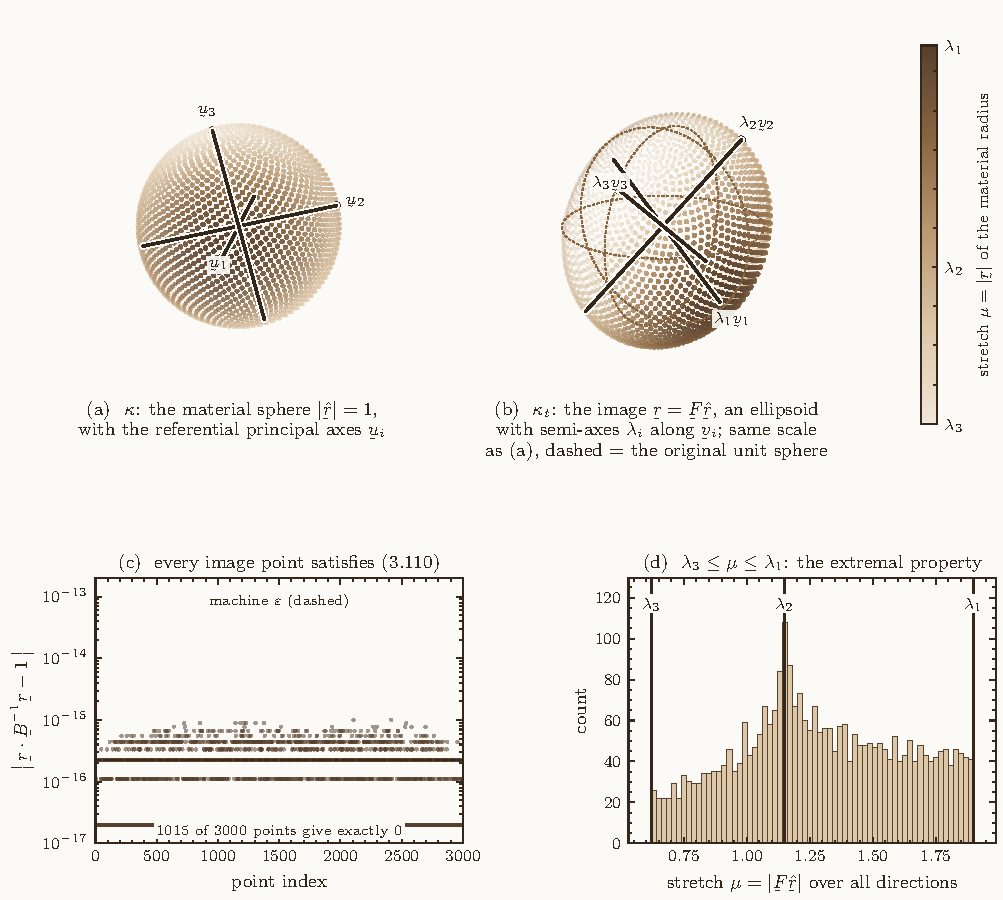
\includegraphics[width=\textwidth]{sphere_to_ellipsoid.pdf}
\caption{Property (c) tested numerically, by the script
\texttt{sphere\_to\_ellipsoid.py}. Three thousand points are spread over
the unit material sphere by a golden-angle spiral and pushed forward by
one fixed $\bF=\bR\bU$ with principal stretches
$\lambda=(1.90,\,1.15,\,0.62)$ and $J=\det\bF=1.3547$. Every marker in
the figure is an individual vector point, not a raster image.
(a) the sphere in $\kappa$, each point shaded by the stretch that material
radius will undergo, with the referential principal axes $\bu_{i}$.
(b) the image in $\kappa_{t}$, at the same scale, with the original sphere
retained as dashed great circles for comparison; the point cloud lies on
an ellipsoid with semi-axes $\lambda_{i}$ along $\bv_{i}$, exactly as
\eqr{3.112} asserts.
(c) the residual $|\ip{\br}{\bB^{-1}\br}-1|$ of \eqr{3.110} for every one of
the three thousand image points, at or below machine precision throughout,
with $1015$ of them exactly zero.
(d) the distribution of the stretch $\mu=|\bF\hat\br|$ over all directions,
confined between $\lambda_{3}$ and $\lambda_{1}$ as the extremal property
\eqr{3.26} requires, with $\lambda_{2}$ falling inside.}
\label{fig:numellipsoid}
\end{figure}

\begin{remark}[what the numerical test in Figure~\ref{fig:numellipsoid}
actually checks]\label{rem:numcheck}
Panels (c) and (d) are the substance; (a) and (b) only make the result
visible. Four separate predictions of the text are tested, and all four
hold to about $10^{-15}$:

$\bullet$\ \ \eqr{3.110}, $\ip{\br}{\bB^{-1}\br}=1$, panel (c);

$\bullet$\ \ \eqr{3.112}, $\sum_{i}(r_{i}/\lambda_{i})^{2}=1$ with
$r_{i}=\ip{\bv_{i}}{\br}$, the same statement resolved on the principal
frame;

$\bullet$\ \ \eqr{3.17}, $\lambda_{1}\lambda_{2}\lambda_{3}=J$, so that the
ellipsoid volume $\tfrac43\pi\lambda_{1}\lambda_{2}\lambda_{3}$ is exactly
$J$ times the sphere volume;

$\bullet$\ \ \eqr{3.44}, $\bF\bu_{i}=\lambda_{i}\bv_{i}$, so the axes really
are the images of the referential principal directions.

One check is deliberately \emph{not} at machine precision, and it should
not be. The semi-axis lengths measured from the cloud, $\max_{\text{cloud}}
|\ip{\bv_{i}}{\br}|$, come out about $4\times10^{-4}$ below $\lambda_{i}$.
That is not an error in \eqr{3.112} but a consequence of sampling: with
finitely many points, none lands exactly on an axis tip, so the measured
semi-axis always undershoots. The script confirms the diagnosis by
refining the cloud, and the discrepancy falls from $3.3\times10^{-4}$ at
$N=3000$ to $1.8\times10^{-5}$ at $N=30\,000$ and
$1.5\times10^{-6}$ at $N=300\,000$, that is like $1/N$.
Distinguishing a discretisation error from a genuine one is the whole
skill of testing a formula numerically.

The script also runs the test backwards. It builds $\bF$ from a chosen
$\bR$ and $\bU$, then throws them away and recovers them from $\bF$ alone
by Theorem~\ref{thm:Uclosed}, that is by the closed form
$\bU=(-\bC^{2}+(i_{1}^{2}-i_{2})\bC+i_{1}i_{3}\hI)/(i_{1}i_{2}-i_{3})$ with
$i_{1}$ from the quartic $(\ast_{2})$. The recovered $\bU$ and $\bR$ agree
with the originals to $5\times10^{-15}$, $\bR^{t}\bR=\hI$ and
$\det\bR=1$ hold to the same order, and both $\bF=\bR\bU$ and
$\bF=\bV\bR$ are reproduced. So the closed form of \S3.4 is not merely
derived, it is executed.
\end{remark}

\begin{remark}[the ellipsoid is the picture of the polar decomposition]
\label{rem:ellipsoid}
Property (c) is $\bF=\bV\bR$ drawn. The rotation $\bR$ takes the unit
sphere to the unit sphere, since it preserves lengths, and therefore
contributes nothing to the shape; all of the shape comes from $\bV$, which
stretches the sphere by $\lambda_{i}$ along $\bv_{i}$. Conversely, if one
measures the ellipsoid in $\kappa_{t}$ one recovers $\bV$ completely and
$\bR$ not at all. This is exactly the sense in which the ellipsoid, and
not $\bF$, is what the material experiences.
\end{remark}

%=======================================================================
\section{Rigid-body motions}\label{sec:rigid}
%=======================================================================

\subsection*{Where we are and why this section closes the chapter}

The chapter opened with a promise: separate the part of $\bF$ that a
material feels from the part it does not. \S3.4 delivered the separation,
$\bF=\bR\bU$, and asserted that $\bR$ is the part that costs nothing. That
assertion has not yet been proved. This section proves it, in the sharpest
possible form: the motions in which \emph{nothing at all} happens to the
material are exactly the motions with $\bU=\hI$, that is exactly the
motions in which $\bF$ is a rotation. Once that is established, the case
for writing constitutive laws in terms of $\bC$ rather than $\bF$ is
complete, and the chapter is finished.

The logic runs the opposite way from \S3.6. There we assumed something
about $\bF$ and deduced geometry; here we assume something purely
geometric, that distances are preserved, and deduce what $\bF$ must be.

A motion is \emph{rigid} if it preserves the distance between every pair of
material points, i.e.\ if
$|\bchi_{\kappa}(\bY,t)-\bchi_{\kappa}(\bX,t)|=|\bY-\bX|$, or, squaring to
remove the square root,
\begin{equation}
   \ip{[\bchi_{\kappa}(\bY,t)-\bchi_{\kappa}(\bX,t)]}
      {[\bchi_{\kappa}(\bY,t)-\bchi_{\kappa}(\bX,t)]}
   =\ip{(\bY-\bX)}{(\bY-\bX)}
   \tag{3.113}\label{eq:3.113}
\end{equation}
for all $\bX,\bY$. Squaring is not cosmetic: the square root in the
definition is awkward to differentiate at $\bY=\bX$, whereas the quadratic
form on each side of \eqr{3.113} is a polynomial and differentiates cleanly.

\emph{The plan.} We have a functional equation, \eqr{3.113}, holding for all
pairs of points, and we want a statement about $\bF$. The route is to
differentiate twice, once with respect to $\bY$ and once with respect to
$\bX$, because each differentiation converts a difference of positions
into an $\bF$, by the definition $\dl\bchi_{\kappa}=\bF\,\dl\bX$. Two
differentiations therefore produce a relation between two $\bF$'s, and that
relation will turn out to say both that $\bF$ is orthogonal and that it
does not vary.

\emph{First differentiation.} Differentiate \eqr{3.113}. Both sides have the
form $\ip\ba\ba$, whose differential is
$\dl(\ip\ba\ba)=\ip{\dl\ba}{\ba}+\ip{\ba}{\dl\ba}=2\ip{\ba}{\dl\ba}$, the
two terms being equal because the dot product is symmetric. The factor $2$
appears on both sides and cancels, leaving
\begin{equation}
   \ip{[\bchi_{\kappa}(\bY,t)-\bchi_{\kappa}(\bX,t)]}
      {\dl[\bchi_{\kappa}(\bY,t)-\bchi_{\kappa}(\bX,t)]}
   =\ip{(\bY-\bX)}{\dl(\bY-\bX)},
   \tag{3.114}\label{eq:3.114}
\end{equation}
in which the derivative may be taken with respect to $\bX$ or to $\bY$; we
choose $\bY$ first.

So fix $\bX$, which makes $\bchi_{\kappa}(\bX,t)$ a constant vector, and
let $\bY$ vary. Then
\[
   \dl\big[\bchi_{\kappa}(\bY,t)-\bchi_{\kappa}(\bX,t)\big]
   =\dl\bchi_{\kappa}(\bY,t)-\bze=\bF(\bY,t)\,\dl\bY,
   \qquad
   \dl(\bY-\bX)=\dl\bY ,
\]
the first by the definition \eqr{2.34} of the deformation gradient at the
point $\bY$. Substituting into \eqr{3.114},
\begin{equation}
   \ip{[\bchi_{\kappa}(\bY,t)-\bchi_{\kappa}(\bX,t)]}{\bF(\bY,t)\dl\bY}
   =\ip{(\bY-\bX)}{\dl\bY}
   \tag{3.115}\label{eq:3.115}
\end{equation}
for all $\dl\bY$. Move $\bF$ to the other factor by the definition of the
transpose, $\ip{\ba}{\bF\bb}=\ip{\bF^{t}\ba}{\bb}$, and collect:
\[
   \ip{\Big(\bF^{t}(\bY,t)\big[\bchi_{\kappa}(\bY,t)
      -\bchi_{\kappa}(\bX,t)\big]-(\bY-\bX)\Big)}{\dl\bY}=0
   \quad\text{for all }\dl\bY .
\]
A vector orthogonal to every vector is $\bze$, so the bracket vanishes:
\begin{equation}
   \bF^{t}(\bY,t)\big[\bchi_{\kappa}(\bY,t)-\bchi_{\kappa}(\bX,t)\big]
   =\bY-\bX .
   \tag{3.116}\label{eq:3.116}
\end{equation}

\emph{Second differentiation.} Now reverse the roles: fix $\bY$, so that
$\bF^{t}(\bY,t)$ and $\bchi_{\kappa}(\bY,t)$ are both constant, and
differentiate \eqr{3.116} with respect to $\bX$. On the left, the only
$\bX$-dependent piece is $-\bchi_{\kappa}(\bX,t)$, whose differential is
$-\bF(\bX,t)\dl\bX$, and the constant tensor $\bF^{t}(\bY,t)$ multiplies
it. On the right, the only $\bX$-dependent piece is $-\bX$. Hence
\[
   -\bF^{t}(\bY,t)\bF(\bX,t)\,\dl\bX=-\dl\bX
   \qquad\text{for all }\dl\bX ,
\]
and cancelling the minus signs and using once more that two tensors
agreeing on every vector are equal,
\begin{equation}
   \bF^{t}(\bY,t)\bF(\bX,t)=\hI\qquad\text{for all }\bX,\bY\in\kappa .
   \tag{3.117}\label{eq:3.117}
\end{equation}
Putting $\bY=\bX$,
\begin{equation}
   \bF^{t}(\bX,t)\bF(\bX,t)=\hI\qquad\text{for all }\bX\in\kappa ,
   \tag{3.118}\label{eq:3.118}
\end{equation}
so $\bF(\bX,t)$ is orthogonal at every $\bX$ and $\bF^{t}=\bF^{-1}$.
Substituting this back into \eqr{3.117} gives
$\bF^{-1}(\bY,t)\bF(\bX,t)=\hI$, i.e.
\begin{equation}
   \bF(\bY,t)=\bF(\bX,t)\qquad\text{for all }\bX,\bY\in\kappa ,
   \tag{3.119}\label{eq:3.119}
\end{equation}
so $\bF$ does not depend on $\bX$ at all:
\begin{equation}
   \bF(\bX,t)=\bQ(t),
   \tag{3.120}\label{eq:3.120}
\end{equation}
a uniform orthogonal tensor, and a rotation if $\kappa$ is occupiable, by
\eqr{2.50}. Rigid motions are therefore homogeneous, and \eqr{3.100} gives
\begin{equation}
   \bx=\bchi_{\kappa}(\bX,t)=\bQ(t)\bX+\bc(t).
   \tag{3.121}\label{eq:3.121}
\end{equation}
Conversely, substituting \eqr{3.121} into the left side of \eqr{3.113} gives
$\ip{\bQ(\bY-\bX)}{\bQ(\bY-\bX)}=\ip{(\bY-\bX)}{\bQ^{t}\bQ(\bY-\bX)}
=\ip{(\bY-\bX)}{(\bY-\bX)}$, so \eqr{3.121} is necessary \emph{and}
sufficient for rigidity.

The polar decomposition is trivial in this case:
\begin{equation}
   \bR=\bQ,\qquad \bU=\hI,\qquad \bV=\I,
   \tag{3.122}\label{eq:3.122}
\end{equation}
and of course $\bC=\hI$ and $\bB=\I$. Uniqueness makes this immediate:
$\bQ=\bQ\hI$ is a factorisation of the required type, hence \emph{the}
one.

\bookfig{7}\begin{figure}[htbp]\centering
\begin{tikzpicture}[scale=1.0,
  vec/.style={-{Stealth[length=2.2mm]},thick},
  lbl/.style={fill=white,inner sep=1pt,font=\small}]
\begin{scope}
\blob{thick}
\coordinate (X) at (-0.35,0.30);
\coordinate (Y) at (0.85,-0.45);
\fill (X) circle (1pt); \fill (Y) circle (1pt);
\node[lbl,left] at (X) {$\bX$}; \node[lbl,right] at (Y) {$\bY$};
\draw[thick] (X)--(Y);
\node[lbl,font=\small] at (0.32,0.05) {$\ell$};
\node[lbl] at (0,-1.65) {$\kappa$};
\end{scope}
\draw[-{Stealth[length=2.6mm]},thick,gray!70] (2.1,0)--(3.5,0);
\node[lbl,above,text=gray!85] at (2.8,0.05) {$\bchi_{\kappa}$};
\begin{scope}[xshift=6.1cm,rotate=-34]
\blob{thick}
\coordinate (X2) at (-0.35,0.30);
\coordinate (Y2) at (0.85,-0.45);
\fill (X2) circle (1pt); \fill (Y2) circle (1pt);
\draw[thick] (X2)--(Y2);
\end{scope}
\node[lbl] at (6.1,-1.65) {$\kappa_{t}$};
\node[lbl,font=\small] at (6.5,0.55) {same $\ell$};
\end{tikzpicture}
\caption{Rigid-body motion. Every material distance is
preserved, so the body may translate and turn but cannot change shape. The
computation \eqr{3.113} to \eqr{3.120} shows that this forces $\bF$ to be a
uniform rotation, hence $\bU=\hI$ and $\bC=\hI$: no stretching anywhere.}
\label{fig:37}
\end{figure}

\begin{remark}[why this is the theorem the whole chapter was for]
\label{rem:rigidwhy}
\eqr{3.122} says: rigid motion $\iff$ $\bU=\hI$ $\iff$ $\bC=\hI$ $\iff$
$\bE=\hOb$. The strain tensors vanish exactly on motions in which nothing
happens to the material. That is the property one demands of a strain
measure, and it is why $\bE=\tfrac12(\bC-\hI)$ was defined with the $\hI$
subtracted. Note what is \emph{not} true: $\bF=\I$ is not the condition
for rigidity, since $\bF=\bQ(t)$ with $\bQ\neq\I$ is rigid too. A
constitutive law written in terms of $\bF$ would therefore assign energy
to a body that is merely being carried around; a law written in terms of
$\bC$ cannot. This is the whole reason for \S3.4.
\end{remark}

%=======================================================================
\section{Problems}\label{sec:problems}
%=======================================================================

All nine problems of the chapter are solved below in the book's order and
notation. They fall into three groups, and it helps to know which is which
before starting.

\emph{Problems 1, 4, 5, 6 are further worked deformations}, in the style of
\S3.5: write down $\bx$, differentiate, read off $\bF$, then extract what
is asked. The recipe of \S3.5 applies verbatim, and rules (R1)--(R4) are
used throughout. Problem 1 adds area change through Piola--Nanson,
Problem 4 is spherically symmetric rather than cylindrical, Problem 5 is a
fourth shear, and Problem 6 is bending.

\emph{Problems 2, 7, 8 are algebra}, filling gaps that \S\S3.1--3.4 left
open: that products of rotations are rotations, which was used at \eqr{3.95};
that the invariants are the elementary symmetric functions of the
principal values, which was used at \eqr{3.17} and in
Remark~\ref{rem:invgeom}; and the Cayley--Hamilton theorem, which is what
makes Theorem~\ref{thm:Uclosed} and Problem 9 possible.

\emph{Problems 3 and 9 are the pay-off.} Problem 3 completes torsion, and
Problem 9 produces the closed form for $\bU$ that removes eigenvectors from
the subject entirely, in two dimensions; Theorem~\ref{thm:Uclosed} did the
same in three.

%-----------------------------------------------------------------------
\begin{problem}[Triaxial stretch: area change and normals]
Consider the deformation $x_{1}=\lambda_{1}X_{1}$,
$x_{2}=\lambda_{2}X_{2}$, $x_{3}=\lambda_{3}X_{3}$ with constant
$\lambda_{i}$ and $\{\be_{i}\}=\{\bE_{A}\}$.
(a) Obtain $\bF$ and state a restriction on the $\lambda_{i}$ for the
deformation to be physically possible.
(b) With $\lambda_{3}=\lambda_{2}$ and the deformation isochoric, consider
a plane material surface in $\kappa$ whose unit normal is inclined at
angle $\phi$ to the $1$-axis. Find, in terms of $\lambda_{1}$ and $\phi$,
the ratio of its deformed area to its undeformed area.
(c) What is the unit normal to that surface after deformation?
\end{problem}

\begin{solution}
\textbf{(a)} Differentiating the three relations at fixed $t$,
$\dl x_{i}=\lambda_{i}\dl X_{i}$ (no sum), and
$\dl X_{A}=\ip{\hbE_{A}}{\dl\bX}$, so
\[
   \dl\bx=\dl x_{i}\be_{i}
   =\sum_{A=1}^{3}\lambda_{A}\,\be_{A}\,(\ip{\hbE_{A}}{\dl\bX})
   =\Big(\sum_{A=1}^{3}\lambda_{A}\,\be_{A}\otimes\hbE_{A}\Big)\dl\bX ,
\]
whence
\[
   \bF=\lambda_{1}\,\be_{1}\otimes\hbE_{1}
      +\lambda_{2}\,\be_{2}\otimes\hbE_{2}
      +\lambda_{3}\,\be_{3}\otimes\hbE_{3}.
\]
This is already in the form \eqr{3.43} with orthonormal frames on both
sides, so if the $\lambda_{A}$ are positive they \emph{are} the principal
stretches, $\bU=\sum\lambda_{A}\hbE_{A}\otimes\hbE_{A}$,
$\bV=\sum\lambda_{A}\be_{A}\otimes\be_{A}$ and $\bR=\shift$. The Jacobian
is
obtained as follows. First the images of the referential frame, each by
(R1) applied to the three dyads:
\[
   \bF\hbE_{1}=\lambda_{1}\be_{1},\qquad
   \bF\hbE_{2}=\lambda_{2}\be_{2},\qquad
   \bF\hbE_{3}=\lambda_{3}\be_{3},
\]
since for instance $\bF\hbE_{1}=\lambda_{1}(\ip{\hbE_{1}}{\hbE_{1}})\be_{1}
+\lambda_{2}(\ip{\hbE_{2}}{\hbE_{1}})\be_{2}
+\lambda_{3}(\ip{\hbE_{3}}{\hbE_{1}})\be_{3}
=\lambda_{1}\be_{1}$. Then rule (R4), with the denominator
$\tbox{\hbE_{1}}{\hbE_{2}}{\hbE_{3}}=1$ by Lemma~\ref{lem:boxortho} and
the scalars taken out one slot at a time by (R3):
\[
\begin{aligned}
   J=\det\bF
   &=\frac{\tbox{\bF\hbE_{1}}{\bF\hbE_{2}}{\bF\hbE_{3}}}
          {\tbox{\hbE_{1}}{\hbE_{2}}{\hbE_{3}}}
    =\frac{\tbox{\lambda_{1}\be_{1}}{\lambda_{2}\be_{2}}
                {\lambda_{3}\be_{3}}}{1}\\
   &=\lambda_{1}\lambda_{2}\lambda_{3}\,
     \tbox{\be_{1}}{\be_{2}}{\be_{3}}
    =\lambda_{1}\lambda_{2}\lambda_{3}\cdot1
    =\lambda_{1}\lambda_{2}\lambda_{3}.
\end{aligned}
\]
\subsubsection*{The restriction on the $\lambda_{A}$}

Two requirements, excluding different things.

\emph{Invertibility.} If $\lambda_{1}=0$ then $\hbE_{1}$ and $2\hbE_{1}$
both map to $\bze$, contradicting \eqr{2.1}. So $\lambda_{A}\neq0$ and
$J\neq0$.

\emph{Sign.} Along a motion, $\bF(t_{0})=\shift$ by \eqr{2.79}, so
$J(t_{0})=1>0$. Now $J(t)$ is continuous and never zero, so by the
intermediate value theorem it cannot change sign. Hence
\[
   \boxed{\ J=\lambda_{1}\lambda_{2}\lambda_{3}>0\ }
\]

This is weaker than $\lambda_{A}>0$. Assuming no signs,
\[
   \bC=\sum_{A}\lambda_{A}^{2}\,\hbE_{A}\otimes\hbE_{A},
   \qquad
   \bU=\sqrt{\bC}=\sum_{A}|\lambda_{A}|\,\hbE_{A}\otimes\hbE_{A},
\]
the positive root by Theorem~\ref{thm:sqrt}, and with
$s_{A}=\operatorname{sgn}\lambda_{A}$,
\[
\begin{aligned}
   \bR&=\bF\bU^{-1}
   =\sum_{A}\frac{\lambda_{A}}{|\lambda_{A}|}\,\be_{A}\otimes\hbE_{A}
   =\sum_{A}s_{A}\,\be_{A}\otimes\hbE_{A},\\
   \det\bR&=s_{1}s_{2}s_{3}=\operatorname{sgn}J .
\end{aligned}
\]
So $\bR$ is a rotation exactly when $J>0$. The four sign patterns:
\[
\begin{array}{cccl}
   (s_{A}) & J & \bR & \\[1mm]
   (+,+,+) & >0 & \shift & \text{pure stretch}\\
   (-,+,+) & <0 & \operatorname{diag}(-1,1,1) & \text{mirror, excluded}\\
   (-,-,+) & >0 & \operatorname{diag}(-1,-1,1) &
     \text{half turn about }\be_{3},\ \text{admissible}\\
   (-,-,-) & <0 & -\shift & \text{inversion, excluded}
\end{array}
\]
The stretches are $|\lambda_{A}|$, not $\lambda_{A}$. Parts (b) and (c)
speak of stretches, so take $\lambda_{A}>0$ below.


\begin{figure}[htbp]\centering
\renewcommand{\thefigure}{E}
\begin{tikzpicture}[x={(-0.50cm,-0.36cm)},y={(1cm,-0.20cm)},z={(0cm,1cm)},
  scale=1.22,
  vec/.style={-{Stealth[length=2.4mm]},thick},
  lbl/.style={fill=white,inner sep=1pt,font=\small}]
% ---------------- reference cube ----------------
\begin{scope}
\fill[gray!10] (0,0,0)--(1,0,0)--(1,1,0)--(0,1,0)--cycle;
\fill[gray!16] (0,0,0)--(1,0,0)--(1,0,1)--(0,0,1)--cycle;
\fill[gray!8]  (0,0,0)--(0,1,0)--(0,1,1)--(0,0,1)--cycle;
\draw[thin,gray!70] (0,0,0)--(1,0,0)--(1,1,0)--(0,1,0)--cycle;
\draw[thin,gray!70] (0,0,1)--(1,0,1)--(1,1,1)--(0,1,1)--cycle;
\foreach \a/\b in {0/0,1/0,1/1,0/1}
  \draw[thin,gray!70] (\a,\b,0)--(\a,\b,1);
\draw[vec] (0,0,0)--(1.55,0,0); \node[lbl] at (1.80,0,0) {$\hbE_{1}$};
\draw[vec] (0,0,0)--(0,1.55,0); \node[lbl] at (0,1.80,0) {$\hbE_{2}$};
\draw[vec] (0,0,0)--(0,0,1.55); \node[lbl] at (0,0,1.80) {$\hbE_{3}$};
\node[font=\small,align=center] at (0.5,0.5,-1.32)
  {$\kappa$: the unit cube,\\
   $\tbox{\hbE_{1}}{\hbE_{2}}{\hbE_{3}}=+1$};
\end{scope}
% ---------------- two negative: admissible ----------------
\begin{scope}[yshift=3.6cm]
\fill[gray!10] (0,0,0)--(-1.5,0,0)--(-1.5,-1.1,0)--(0,-1.1,0)--cycle;
\fill[gray!16] (0,0,0)--(-1.5,0,0)--(-1.5,0,0.7)--(0,0,0.7)--cycle;
\draw[thin,gray!70] (0,0,0)--(-1.5,0,0)--(-1.5,-1.1,0)--(0,-1.1,0)--cycle;
\draw[thin,gray!70] (0,0,0.7)--(-1.5,0,0.7)--(-1.5,-1.1,0.7)--(0,-1.1,0.7)
  --cycle;
\foreach \a/\b in {0/0,-1.5/0,-1.5/-1.1,0/-1.1}
  \draw[thin,gray!70] (\a,\b,0)--(\a,\b,0.7);
\draw[vec] (0,0,0)--(-2.0,0,0); \node[lbl] at (-2.35,0,0) {$\lambda_{1}\be_{1}$};
\draw[vec] (0,0,0)--(0,-1.6,0); \node[lbl] at (0,-1.95,0) {$\lambda_{2}\be_{2}$};
\draw[vec] (0,0,0)--(0,0,1.2); \node[lbl] at (0,0,1.45) {$\lambda_{3}\be_{3}$};
\node[font=\small,align=center] at (-0.75,-0.55,-1.32)
  {$\lambda=(-1.5,\,-1.1,\,0.7)$:\ \
   $\tbox{\bF\hbE_{1}}{\bF\hbE_{2}}{\bF\hbE_{3}}=+1.155$\\
   still right handed; $\bR$ is the half turn about $\be_{3}$
   \ \checkmark};
\end{scope}
% ---------------- one negative: inadmissible ----------------
\begin{scope}[yshift=7.6cm]
\fill[gray!10] (0,0,0)--(-1.5,0,0)--(-1.5,1.1,0)--(0,1.1,0)--cycle;
\fill[gray!16] (0,0,0)--(-1.5,0,0)--(-1.5,0,0.7)--(0,0,0.7)--cycle;
\draw[thin,gray!70] (0,0,0)--(-1.5,0,0)--(-1.5,1.1,0)--(0,1.1,0)--cycle;
\draw[thin,gray!70] (0,0,0.7)--(-1.5,0,0.7)--(-1.5,1.1,0.7)--(0,1.1,0.7)
  --cycle;
\foreach \a/\b in {0/0,-1.5/0,-1.5/1.1,0/1.1}
  \draw[thin,gray!70] (\a,\b,0)--(\a,\b,0.7);
\draw[vec] (0,0,0)--(-2.0,0,0); \node[lbl] at (-2.35,0,0) {$\lambda_{1}\be_{1}$};
\draw[vec] (0,0,0)--(0,1.6,0); \node[lbl] at (0,1.95,0) {$\lambda_{2}\be_{2}$};
\draw[vec] (0,0,0)--(0,0,1.2); \node[lbl] at (0,0,1.45) {$\lambda_{3}\be_{3}$};
\node[font=\small,align=center] at (-0.75,0.55,-1.32)
  {$\lambda=(-1.5,\,1.1,\,0.7)$:\ \
   $\tbox{\bF\hbE_{1}}{\bF\hbE_{2}}{\bF\hbE_{3}}=-1.155$\\
   now left handed; $\bR$ is a mirror \ $\times$};
\end{scope}
\end{tikzpicture}
\caption{Why the restriction is $\lambda_{1}\lambda_{2}\lambda_{3}>0$ and
not $\lambda_{A}>0$. Bottom, the reference cube with its right-handed
frame. Middle, two of the $\lambda$'s negative: the frame is turned
through $\pi$ about $\be_{3}$ but is still right handed, the box product
is still positive, and the deformation is a genuine one, a pure stretch
followed by a half turn. Top, one $\lambda$ negative: the frame has become
left handed, the box product is negative, and $\bR$ is a mirror. No
continuous motion starting from $\bF=\shift$ can reach it, because $J$
would have to pass through zero and $\bF$ would cease to be invertible at
that instant.}
\label{fig:signs}
\end{figure}

\textbf{(b)} Isochoric with $\lambda_{3}=\lambda_{2}$ means
$\lambda_{1}\lambda_{2}^{2}=1$, so
\[
   \lambda_{2}=\lambda_{3}=\lambda_{1}^{-1/2}.
\]
Take the normal in the $(1,2)$ plane without loss of generality, since the
$2$ and $3$ directions are now equivalent:
\[
   \bN=\cos\phi\,\hbE_{1}+\sin\phi\,\hbE_{2}.
\]
The Piola--Nanson formula \eqr{2.54} with \eqr{2.55} gives
$\bn\,\dl a=\bF^{*}\bN\,\dl A$ and $\bF^{*}=J\bF^{-t}=\bF^{-t}$ since
$J=1$. From the dyadic form of $\bF$,
\[
   \bF^{-1}=\sum_{A}\lambda_{A}^{-1}\,\hbE_{A}\otimes\be_{A},
   \qquad
   \bF^{-t}=\sum_{A}\lambda_{A}^{-1}\,\be_{A}\otimes\hbE_{A},
\]
the first because
\[
   \Big(\sum_{A}\lambda_{A}^{-1}\hbE_{A}\otimes\be_{A}\Big)
   \Big(\sum_{B}\lambda_{B}\be_{B}\otimes\hbE_{B}\Big)
   =\sum_{A,B}\lambda_{A}^{-1}\lambda_{B}\dd_{AB}
    \,\hbE_{A}\otimes\hbE_{B}=\hI .
\]
Therefore
\[
   \bF^{*}\bN=\lambda_{1}^{-1}\cos\phi\,\be_{1}
             +\lambda_{2}^{-1}\sin\phi\,\be_{2},
\]
and taking the length of both sides of $\bn\,\dl a=\bF^{*}\bN\,\dl A$,
with $|\bn|=1$,
\[
   \frac{\dl a}{\dl A}=|\bF^{*}\bN|
   =\sqrt{\lambda_{1}^{-2}\cos^{2}\phi+\lambda_{2}^{-2}\sin^{2}\phi}
   =\boxed{\ \sqrt{\lambda_{1}^{-2}\cos^{2}\phi+\lambda_{1}\sin^{2}\phi}\ }
\]
where $\lambda_{2}^{-2}=(\lambda_{1}^{-1/2})^{-2}=\lambda_{1}$ was used.

Checks. At $\lambda_{1}=1$ the deformation is the identity and the formula
gives $\sqrt{\cos^{2}\phi+\sin^{2}\phi}=1$. At $\phi=0$ the surface is
normal to the stretching axis and the ratio is $\lambda_{1}^{-1}$, which
is right: that face has area $\lambda_{2}\lambda_{3}=\lambda_{1}^{-1}$
times its original. At $\phi=\pi/2$ the ratio is $\lambda_{1}^{1/2}
=\lambda_{1}\lambda_{3}=\lambda_{1}\lambda_{1}^{-1/2}$, also right.

\textbf{(c)} Dividing $\bF^{*}\bN$ by its length,
\[
   \bn=\frac{\lambda_{1}^{-1}\cos\phi\,\be_{1}
             +\lambda_{1}^{1/2}\sin\phi\,\be_{2}}
            {\sqrt{\lambda_{1}^{-2}\cos^{2}\phi+\lambda_{1}\sin^{2}\phi}},
\]
using $\lambda_{2}^{-1}=\lambda_{1}^{1/2}$. Equivalently, the deformed
normal makes an angle $\psi$ with the $1$-axis given by
\[
   \tan\psi=\lambda_{1}^{3/2}\tan\phi .
\]
Note that the normal does \emph{not} rotate the way the material does: for
$\lambda_{1}>1$ it turns \emph{away} from the stretching axis, because
$\bF^{-t}$, not $\bF$, transports normals. This is the standard trap that
Piola--Nanson exists to avoid.
\end{solution}

%-----------------------------------------------------------------------
\begin{problem}[Products of orthogonal tensors]
Prove that the product of two orthogonal tensors is orthogonal, and that
the product of two rotations is a rotation.
\end{problem}

\begin{solution}
Let $\bQ_{1},\bQ_{2}$ be orthogonal, meaning $\bQ_{k}^{t}\bQ_{k}=\I$.
Using $(\bA\bB)^{t}=\bB^{t}\bA^{t}$ from Problem 20 of Chapter 1 and
associativity,
\[
   (\bQ_{1}\bQ_{2})^{t}(\bQ_{1}\bQ_{2})
   =\bQ_{2}^{t}\bQ_{1}^{t}\bQ_{1}\bQ_{2}
   =\bQ_{2}^{t}\,\I\,\bQ_{2}
   =\bQ_{2}^{t}\bQ_{2}=\I ,
\]
so $\bQ_{1}\bQ_{2}$ is orthogonal.

Two gaps to close. First, $\bQ^{t}\bQ=\I$ implies $\bQ\bQ^{t}=\I$: if
$\bQ\ba=\bze$ then $\ba=\bQ^{t}\bQ\ba=\bze$, so $\bQ$ is injective, hence
bijective in finite dimensions, hence $\bQ^{-1}=\bQ^{t}$ and
$\bQ\bQ^{t}=\I$. Second, $\det\bQ^{t}\det\bQ=\det\I=1$ with
$\det\bQ^{t}=\det\bQ$ gives $(\det\bQ)^{2}=1$, so $\det\bQ=\pm1$.

\emph{What orthogonality means.} The three statements
\[
   \bQ^{t}\bQ=\I,
   \qquad
   \ip{\bQ\ba}{\bQ\bb}=\ip\ba\bb\ \ \forall\ba,\bb,
   \qquad
   |\bQ\ba|=|\ba|\ \ \forall\ba
\]
are equivalent. The first gives the second by
$\ip{\bQ\ba}{\bQ\bb}=\ip{\ba}{\bQ^{t}\bQ\bb}=\ip\ba\bb$; the second gives
the third at $\bb=\ba$; and the third gives the second by polarisation,
\[
   \ip\ba\bb=\tfrac12\big(|\ba+\bb|^{2}-|\ba|^{2}-|\bb|^{2}\big),
\]
each term of which is preserved. The second then gives the first, since
$\ip{\ba}{(\bQ^{t}\bQ-\I)\bb}=0$ for all $\ba,\bb$. So a product of
orthogonal tensors is orthogonal for a reason needing no algebra: doing
two length-preserving maps in succession preserves lengths.

A \emph{rotation} is an orthogonal tensor with $\det=+1$. By Problem 21(b)
of Chapter 1,
\[
   \det(\bQ_{1}\bQ_{2})=(\det\bQ_{1})(\det\bQ_{2})=(+1)(+1)=+1 ,
\]
so a product of rotations is a rotation.

The version actually used at \eqr{3.95} is the two-point one: if
$\bQ_{1}\in\Orth(\hVt,\Vt)$ and $\bQ_{2}\in\Orth(\hVt,\hVt)$ then
$\bQ_{1}\bQ_{2}\in\Orth(\hVt,\Vt)$. The computation is identical, the
only change being that $\bQ_{2}^{t}\bQ_{2}=\hI$ and
$\bQ_{1}^{t}\bQ_{1}=\hI$, so the chain reads
$(\bQ_{1}\bQ_{2})^{t}(\bQ_{1}\bQ_{2})=\bQ_{2}^{t}\hI\bQ_{2}=\hI$; and
the determinant statement uses the extension recorded in
Remark~\ref{rem:detext}.
\end{solution}

%-----------------------------------------------------------------------
\begin{problem}[Torsion: Cauchy--Green tensors and principal stretches]
Evaluate the left and right Cauchy--Green tensors for the torsion problem.
Find the principal stretches in terms of the twist $\tau$. Verify that
azimuthal shear and torsion are isochoric.
\end{problem}

\begin{solution}
From \eqr{3.88} and \eqr{3.97}, $\bF=\bQ\hat\bG=\bG\bQ$ with
\[
   \hat\bG=\hI+\gamma\,\hETh\otimes\hbE_{3},\qquad
   \bG=\I+\gamma\,\bet\otimes\be_{3},\qquad \gamma=\gamma(R)=R\tau .
\]
Since $\bQ^{t}\bQ=\hI$ and $\bQ\bQ^{t}=\I$, exactly as in \eqr{3.91},
\[
   \bC=\hat\bG^{t}\bQ^{t}\bQ\hat\bG=\hat\bG^{t}\hat\bG,
   \qquad
   \bB=\bG\bQ\bQ^{t}\bG^{t}=\bG\bG^{t}.
\]
With $\hat\bG^{t}=\hI+\gamma\,\hbE_{3}\otimes\hETh$,
\[
\begin{aligned}
   \bC&=(\hI+\gamma\hbE_{3}\otimes\hETh)(\hI+\gamma\hETh\otimes\hbE_{3})\\
   &=\hI+\gamma\,\hETh\otimes\hbE_{3}+\gamma\,\hbE_{3}\otimes\hETh
     +\gamma^{2}(\ip{\hETh}{\hETh})\,\hbE_{3}\otimes\hbE_{3}\\
   &=\hI+\gamma\big[\hETh(\Theta)\otimes\hbE_{3}
      +\hbE_{3}\otimes\hETh(\Theta)\big]
      +\gamma^{2}\,\hbE_{3}\otimes\hbE_{3},
\end{aligned}
\]
and in the same way
\[
   \bB=\I+\gamma\big[\bet(\theta)\otimes\be_{3}
      +\be_{3}\otimes\bet(\theta)\big]
      +\gamma^{2}\,\bet(\theta)\otimes\bet(\theta).
\]
Note again the shift of the squared term from $\hbE_{3}$ in $\bC$ to
$\bet$ in $\bB$, exactly as in Remark~\ref{rem:CnotB}.

\emph{Principal stretches.} In the orthonormal basis
$\{\hER,\hETh,\hbE_{3}\}$ the matrix of $\bC$ is
\[
   (C_{AB})=\begin{pmatrix}1&0&0\\ 0&1&\gamma\\ 0&\gamma&1+\gamma^{2}
   \end{pmatrix},
\]
which is \eqr{3.55} with the roles of the axes permuted: the shear acts on
the pair $(\hETh,\hbE_{3})$ and $\hER$ is inert. Hence one principal
stretch is $1$, with principal direction $\hER$, and the other two solve
the same quadratic as before. Reading \eqr{3.60} with $\gamma=R\tau$,
\[
   \boxed{\ \lambda_{1}=\tfrac12\big(R\tau+\sqrt{4+R^{2}\tau^{2}}\big),
   \qquad \lambda_{2}=\lambda_{1}^{-1},\qquad \lambda_{3}=1 .\ }
\]
The stretches depend on $R$: fibres near the axis are barely deformed,
fibres near the outer surface most. At $R=0$ all three are $1$, which is
right, since the axis of a twisted bar is not deformed at all.

\emph{Isochoric.} For torsion, by Problem 21(f) of Chapter 1,
\[
   \det\hat\bG=\det(\hI+\gamma\hETh\otimes\hbE_{3})
   =1+\gamma\,\ip{\hETh}{\hbE_{3}}=1+0=1 ,
\]
and $\det\bF=(\det\bQ)(\det\hat\bG)=1\cdot1=1$. For azimuthal shear the
same computation with \eqr{3.88} gives
$\det\hat\bG=1+\gamma\,\ip{\hETh}{\hER}=1$. Both deformations are
isochoric.

An independent check: $\det\bC=(\det\bF)^{2}$ should be $1$. Expanding the
matrix above along the first row,
$\det(C_{AB})=1\cdot[(1)(1+\gamma^{2})-\gamma^{2}]=1$. Consistent.

Geometrically the reason is the one visible in
Remark~\ref{rem:threeshears}: every shear $\hI+\gamma\ba\otimes\bb$ with
$\ba\perp\bb$ slides planes over one another without moving any of them
closer, so no volume can change.
\end{solution}

%-----------------------------------------------------------------------
\begin{problem}[Spherically symmetric deformation]
Consider the static deformation $\bx=\bchi_{\kappa}(\bX)=\lambda(R)\shift
\bX$, where $R=|\bX|$ and $\lambda(R)$ is given.
(a) Describe what it does to a spherical annulus $A\le R\le B$.
(b) Derive $\bF$ and state the restrictions on $\lambda$.
(c) Find $\lambda(R)$ if the deformation is isochoric with
$\lambda(A)=a/A$.
\end{problem}

\begin{solution}
\textbf{(a)} Since $|\bx|=\lambda(R)|\shift\bX|=\lambda(R)R$ and the
direction of $\bx$ is that of $\shift\bX$, every material point moves
along its own radius; the sphere $R=\text{const}$ goes to the sphere
$r=\lambda(R)R$. The annulus $A\le R\le B$ therefore becomes the annulus
$a\le r\le b$ with $a=\lambda(A)A$ and $b=\lambda(B)B$, and each concentric
material sphere remains a concentric sphere. The deformation is a purely
radial inflation or contraction, with no rotation and no distortion of
the angular structure. It is the natural model for a pressurised spherical
shell.

Not a similarity: $\lambda$ depends on $R$, so $\Delta r/\Delta R$ varies.
Every direction perpendicular to $\bN$ is equivalent, so there are only
two distinct stretches, the second repeated: the repeated-root case of
Remark~\ref{rem:proofbuys}.

\begin{figure}[htbp]\centering
\renewcommand{\thefigure}{F}
\begin{tikzpicture}[scale=1.0,
  vec/.style={-{Stealth[length=2.2mm]},thick},
  lbl/.style={fill=white,inner sep=1pt,font=\small}]
% ---------------- reference annulus ----------------
\begin{scope}
\fill[gray!12] (0,0) circle (1.75);
\fill[white] (0,0) circle (0.85);
\draw[thick] (0,0) circle (1.75);
\draw[thick] (0,0) circle (0.85);
\draw[gray!55,thin] (0,0) circle (1.30);
\fill (0,0) circle (0.8pt);
\draw[vec] (0,0)--(58:0.85); \node[lbl,font=\small] at (58:0.52) {$A$};
\draw[vec] (0,0)--(20:1.75); \node[lbl,font=\small] at (20:1.35) {$B$};
\draw[vec,gray!75] (0,0)--(150:1.30);
\node[lbl,font=\small] at (150:0.80) {$R$};
% a material element
\draw[thick,gray!85] (128:1.30) arc (128:112:1.30);
\draw[thick,gray!85] (128:1.52) arc (128:112:1.52);
\draw[thick,gray!85] (128:1.30)--(128:1.52);
\draw[thick,gray!85] (112:1.30)--(112:1.52);
\node[lbl,font=\small] at (120:1.95) {$\dl R\times R\dl\Theta$};
\node[lbl] at (0,-2.15) {$\kappa$};
\end{scope}
% ---------------- arrow ----------------
\draw[-{Stealth[length=2.6mm]},thick,gray!70] (2.35,0)--(3.45,0);
\node[lbl,above,text=gray!85] at (2.90,0.06) {$\bF$};
\node[font=\small,text=gray!85] at (2.90,-0.55) {$r=\lambda(R)R$};
% ---------------- current annulus ----------------
\begin{scope}[xshift=6.1cm]
\fill[gray!12] (0,0) circle (2.25);
\fill[white] (0,0) circle (1.55);
\draw[thick] (0,0) circle (2.25);
\draw[thick] (0,0) circle (1.55);
\draw[gray!55,thin] (0,0) circle (1.88);
\fill (0,0) circle (0.8pt);
\draw[vec] (0,0)--(58:1.55); \node[lbl,font=\small] at (58:1.05) {$a$};
\draw[vec] (0,0)--(20:2.25); \node[lbl,font=\small] at (20:1.80) {$b$};
\draw[vec,gray!75] (0,0)--(150:1.88);
\node[lbl,font=\small] at (150:1.20) {$r$};
\draw[thick,gray!85] (128:1.88) arc (128:112:1.88);
\draw[thick,gray!85] (128:2.02) arc (128:112:2.02);
\draw[thick,gray!85] (128:1.88)--(128:2.02);
\draw[thick,gray!85] (112:1.88)--(112:2.02);
\node[lbl,font=\small,align=center] at (120:2.62)
  {$(\lambda R)'\dl R\times\lambda R\,\dl\Theta$};
\node[lbl] at (0,-2.65) {$\kappa_{t}$};
\end{scope}
\end{tikzpicture}
\caption{Problem 4, on a diametral section. Every point moves along its own
radius, so $A\le R\le B$ goes to $a\le r\le b$ with $a=\lambda(A)A$,
$b=\lambda(B)B$. The element shows the two stretches,
$\dl R\mapsto(\lambda R)'\dl R$ and
$R\,\dl\Theta\mapsto\lambda R\,\dl\Theta$; with the second, equal,
tangential stretch, $J=\lambda^{2}(\lambda R)'$.}
\label{fig:sphdef}
\end{figure}

\textbf{(b)} Write $\bN=\bX/R$, the referential radial unit vector, so
$\shift\bX=R\,\shift\bN$. Differentiating $\bx=\lambda(R)\shift\bX$,
\[
   \dl\bx=\lambda'(R)\,\dl R\;\shift\bX+\lambda(R)\,\shift\,\dl\bX .
\]
The increment $\dl R$ follows from $R^{2}=\ip\bX\bX$: differentiating,
$2R\,\dl R=2\ip{\bX}{\dl\bX}$, so
$\dl R=\ip{(\bX/R)}{\dl\bX}=\ip{\bN}{\dl\bX}$. Hence
\[
   \dl\bx=\lambda'R\,(\shift\bN)(\ip{\bN}{\dl\bX})+\lambda\shift\,\dl\bX
   =\big[\lambda\shift+R\lambda'\,(\shift\bN)\otimes\bN\big]\dl\bX ,
\]
so, writing $\bn_{0}=\shift\bN$ for the shifted radial direction,
\[
   \boxed{\ \bF=\lambda(R)\,\shift+R\lambda'(R)\;\bn_{0}\otimes\bN .\ }
\]
Its action splits cleanly. On the radial direction,
\[
   \bF\bN=\lambda\bn_{0}+R\lambda'(\ip\bN\bN)\bn_{0}
        =(\lambda+R\lambda')\bn_{0}=(\lambda R)'\,\bn_{0},
\]
so the radial stretch is $(\lambda R)'=\dl r/\dl R$ with $r=\lambda R$; on
any $\bM\perp\bN$,
\[
   \bF\bM=\lambda\shift\bM+R\lambda'(\ip\bN\bM)\bn_{0}=\lambda\,\shift\bM,
\]
so the hoop stretch is $\lambda$, twice. The deformation gradient is
therefore already in the form \eqr{3.43}, with
\[
   \bU=(\lambda R)'\,\bN\otimes\bN+\lambda(\hI-\bN\otimes\bN),
   \qquad \bR=\shift ,
\]
using $\hI-\bN\otimes\bN=\Proj{\bN}$, the projection of Problem 10 of
Chapter 1 onto the tangent plane of the sphere. For the Jacobian, take as
test triad $\{\bN,\bM_{1},\bM_{2}\}$, any right-handed orthonormal frame
whose first member is the radial direction, so that $\bM_{1},\bM_{2}$ are
tangent to the sphere. The images were just computed:
$\bF\bN=(\lambda R)'\bn_{0}$, $\bF\bM_{1}=\lambda\shift\bM_{1}$,
$\bF\bM_{2}=\lambda\shift\bM_{2}$. Since $\shift$ is an isometry with
$\det\shift=1$, the triad $\{\bn_{0},\shift\bM_{1},\shift\bM_{2}\}$ is
again right-handed orthonormal, so both box products in (R4) equal $1$ by
Lemma~\ref{lem:boxortho}, and pulling out one scalar per slot,
\[
\begin{aligned}
   J=\det\bF
   &=\frac{\tbox{(\lambda R)'\bn_{0}}{\lambda\shift\bM_{1}}
                {\lambda\shift\bM_{2}}}
          {\tbox{\bN}{\bM_{1}}{\bM_{2}}}
    =\frac{(\lambda R)'\,\lambda\,\lambda\cdot 1}{1}\\
   &=\lambda^{2}(\lambda R)'=\frac{r^{2}r'}{R^{2}},\qquad r=\lambda R ,
\end{aligned}
\]
the last form because $r^{2}/R^{2}=\lambda^{2}$ and $r'=(\lambda R)'$.
Physical possibility requires $J>0$, hence
\[
   \lambda(R)>0\quad\text{and}\quad (\lambda R)'>0 ,
\]
i.e.\ $r(R)$ must be positive and strictly increasing: distinct material
spheres must remain distinct and must not turn inside out.

\textbf{(c)} Isochoric means $J=1$, i.e.\ $r^{2}r'=R^{2}$, i.e.\
$\tfrac13(r^{3})'=\tfrac13(R^{3})'$. Integrating,
\[
   r^{3}-R^{3}=\text{const}.
\]
The condition $\lambda(A)=a/A$ says $r(A)=\lambda(A)A=a$, so the constant
is $a^{3}-A^{3}$ and
\[
   r^{3}=R^{3}+a^{3}-A^{3},
   \qquad\text{that is}\qquad
   \boxed{\ \lambda(R)=\frac{\big(R^{3}+a^{3}-A^{3}\big)^{1/3}}{R}\ }.
\]
Checks. $\lambda(A)=(A^{3}+a^{3}-A^{3})^{1/3}/A=a/A$ as required. If
$a=A$ then $\lambda\equiv1$ and the deformation is the identity, as it
must be, since an isochoric radial deformation that fixes the inner
surface fixes everything. If $a>A$ the shell is inflated, and
$\lambda(R)\to1$ as $R\to\infty$: the disturbance dies away, which is the
familiar statement that an incompressible medium transmits a cavity
expansion as a $1/R^{3}$ perturbation.
\end{solution}

%-----------------------------------------------------------------------
\begin{problem}[Telescopic, or anti-plane, shear]
Consider $\bx=\bchi_{\kappa}(\bX,t)=\shift\bX+w(R,t)\be_{3}$ with
$\bX=R\hER(\Theta)+Z\hbE_{3}$.
(a) Show that $\bF=\shift+\gamma(R,t)\be_{3}\otimes\hER(\Theta)$ with
$\gamma=\partial w/\partial R$, derive $\bC$ and $\bB$, and justify the
terminology.
(b) Find the stretch $\mu$ and current tangent $\bm$ of the material curve
with $M=\tfrac{\sqrt2}{2}[\hETh+\hbE_{3}]$, and the same for
$\bM=\tfrac{\sqrt2}{2}[\hER+\hETh]$.
\end{problem}

\begin{solution}
\textbf{(a)} Differentiating at fixed $t$ and using
$\dl R=\ip{\hER}{\dl\bX}$,
\[
   \dl\bx=\shift\,\dl\bX+\frac{\partial w}{\partial R}\,\dl R\;\be_{3}
   =\big[\shift+\gamma\,\be_{3}\otimes\hER(\Theta)\big]\dl\bX ,
   \qquad \gamma=\frac{\partial w}{\partial R},
\]
so $\bF=\shift+\gamma\,\be_{3}\otimes\hER(\Theta)$ as claimed. Choose the
shifter so that $\shift\hbE_{3}=\be_{3}$ and $\shift\hER=\ber$, which is
the alignment of \eqr{2.79}.

For $\bC$, transpose and multiply, using Problems 17(b),(c) and
$\shift^{t}\be_{3}=\hbE_{3}$:
\[
\begin{aligned}
   \bC=\bF^{t}\bF
   &=(\shift^{t}+\gamma\,\hER\otimes\be_{3})
     (\shift+\gamma\,\be_{3}\otimes\hER)\\
   &=\hI+\gamma\,(\shift^{t}\be_{3})\otimes\hER
     +\gamma\,\hER\otimes(\shift^{t}\be_{3})
     +\gamma^{2}(\ip{\be_{3}}{\be_{3}})\,\hER\otimes\hER\\
   &=\hI+\gamma\big[\hbE_{3}\otimes\hER(\Theta)
     +\hER(\Theta)\otimes\hbE_{3}\big]
     +\gamma^{2}\,\hER(\Theta)\otimes\hER(\Theta),
\end{aligned}
\]
and similarly, with $\shift\hER=\ber$,
\[
\begin{aligned}
   \bB=\bF\bF^{t}
   &=(\shift+\gamma\,\be_{3}\otimes\hER)
     (\shift^{t}+\gamma\,\hER\otimes\be_{3})\\
   &=\I+\gamma\,(\shift\hER)\otimes\be_{3}
     +\gamma\,\be_{3}\otimes(\shift\hER)
     +\gamma^{2}\,\be_{3}\otimes\be_{3}\\
   &=\I+\gamma\big[\ber(\theta)\otimes\be_{3}
     +\be_{3}\otimes\ber(\theta)\big]+\gamma^{2}\,\be_{3}\otimes\be_{3}.
\end{aligned}
\]
This is again a simple shear of amount $\gamma(R,t)$, now on the
orthonormal pair $(\hbE_{3},\hER)$, so everything in
Remark~\ref{rem:threeshears} applies; in particular
$\det\bF=1+\gamma\,\ip{\be_{3}}{\shift\hER}=1+\gamma\,\ip{\be_{3}}{\ber}
=1$ by Problem 21(g) of Chapter 1, so the deformation is isochoric.

\emph{Terminology.} A material point at $(R,\Theta,Z)$ moves to
$(R,\Theta,Z+w(R))$. Its radial and azimuthal coordinates do not change at
all, and the displacement is purely axial, i.e.\ purely \emph{out of} the
$(R,\Theta)$ plane: hence \emph{anti-plane} shear. Since $w$ depends on
$R$ alone, each concentric material cylinder $R=\text{const}$ slides
rigidly along the axis by a different amount, exactly as the sections of
a telescope slide over one another: hence \emph{telescopic} shear.

\textbf{(b)} Both computations use \eqr{2.67}, $\mu\bm=\bF\bM$, with
$\bF\hER=\ber+\gamma\be_{3}$, $\bF\hETh=\bet$, $\bF\hbE_{3}=\be_{3}$,
which follow from $\bF=\shift+\gamma\be_{3}\otimes\hER$ and
$\ip{\hER}{\hETh}=\ip{\hER}{\hbE_{3}}=0$, $\ip{\hER}{\hER}=1$.

\emph{First curve,} $\bM=\tfrac{\sqrt2}{2}(\hETh+\hbE_{3})$:
\[
   \bF\bM=\tfrac{\sqrt2}{2}\big(\bF\hETh+\bF\hbE_{3}\big)
        =\tfrac{\sqrt2}{2}\big(\bet+\be_{3}\big),
   \qquad
   \mu=|\bF\bM|=\tfrac{\sqrt2}{2}\sqrt{1+1}=1 ,
\]
so $\mu=1$ and $\bm=\tfrac{\sqrt2}{2}(\bet+\be_{3})$: \emph{this helix
does not stretch at all}, whatever $\gamma$. The reason is visible in
$\bC$: the shear couples $\hER$ to $\hbE_{3}$, and this $\bM$ has no
$\hER$ component. Confirming with \eqr{2.83},
\[
   \bC\bM=\tfrac{\sqrt2}{2}\big(\hETh+\hbE_{3}+\gamma\hER\big),
   \qquad
   \mu^{2}=\ip\bM{\bC\bM}=\tfrac12(1+1+0)=1 . \checkmark
\]

\emph{Second curve,} $\bM=\tfrac{\sqrt2}{2}(\hER+\hETh)$:
\[
   \bF\bM=\tfrac{\sqrt2}{2}\big(\ber+\gamma\be_{3}+\bet\big),
   \qquad
   \mu=\tfrac{\sqrt2}{2}\sqrt{1+\gamma^{2}+1}
     =\sqrt{1+\tfrac{\gamma^{2}}{2}} ,
\]
and
\[
   \bm=\frac{\ber(\theta)+\bet(\theta)+\gamma\,\be_{3}}
            {\sqrt{2+\gamma^{2}}} .
\]
Confirming with $\bC$: $\bC\hER=(1+\gamma^{2})\hER+\gamma\hbE_{3}$ and
$\bC\hETh=\hETh$, so
\[
\begin{aligned}
   \mu^{2}&=\ip\bM{\bC\bM}
   =\tfrac12\,\ip{(\hER+\hETh)}
    {\big[(1+\gamma^{2})\hER+\gamma\hbE_{3}+\hETh\big]}\\
   &=\tfrac12\big[(1+\gamma^{2})+1\big]=1+\tfrac{\gamma^{2}}{2}
   \quad\checkmark
\end{aligned}
\]
So the curve inclined at $45^{\circ}$ between the radial and azimuthal
directions does stretch, and by a factor that grows with the local shear.
\end{solution}

%-----------------------------------------------------------------------
\begin{problem}[Flexure of a block]
Consider the static deformation $\bX\to\bx$ with $\bX=X_{A}\hbE_{A}$ and
$\bx=r\ber(\theta)+z\be_{3}$, where $r=f(X_{1})>0$, $\theta=g(X_{2})$,
$z=Z=X_{3}$.
(a) Describe the images of the lines $X_{1}=\text{const}$ and
$X_{2}=\text{const}$ and justify calling this a flexure.
(b) Derive $\bF$. (c) Show $\det\bF>0\iff ff'g'>0$.
(d) Assuming $f>0$, $g'>0$, obtain $\bR,\bU,\bV$ by inspection, and find
$f,g$ if the deformation is isochoric.
\end{problem}

\begin{solution}
\textbf{(a)} A line $X_{1}=c_{1}$, along which $X_{2}$ varies, maps to the
set $r=f(c_{1})=\text{const}$ with $\theta=g(X_{2})$ sweeping an interval:
a \emph{circular arc} of radius $f(c_{1})$ centred on the axis. A line
$X_{2}=c_{2}$, along which $X_{1}$ varies, maps to $\theta=g(c_{2})
=\text{const}$ with $r=f(X_{1})$ varying: a \emph{radial straight
segment}. So the two families of coordinate lines of the block go to
concentric arcs and radial rays respectively, and a rectangular block is
carried into an annular wedge. That is precisely bending: parallel planes
become coaxial cylinders and normal cross-sections remain plane and
normal. Hence \emph{flexure}.

Explicitly $(X_{1},X_{2})\mapsto(r,\theta)=(f(X_{1}),g(X_{2}))$, so
\[
\begin{aligned}
   \text{lines } X_{1}=\text{const}\ &\longmapsto\ \text{arcs }
     r=\text{const},\\
   \text{lines } X_{2}=\text{const}\ &\longmapsto\ \text{rays }
     \theta=\text{const}.
\end{aligned}
\]
A block $0\le X_{1}\le T$, $0\le X_{2}\le L$ becomes the wedge
$f(0)\le r\le f(T)$, $g(0)\le\theta\le g(L)$. The bend angle is
$g(L)-g(0)$; the ring closes when it equals $2\pi$.

\begin{figure}[htbp]\centering
\renewcommand{\thefigure}{G}
\begin{tikzpicture}[scale=1.0,
  vec/.style={-{Stealth[length=2.2mm]},thick},
  lbl/.style={fill=white,inner sep=1pt,font=\small}]
% ---------------- the block in kappa ----------------
\begin{scope}
\fill[gray!12] (0,0) rectangle (1.15,3.1);
\draw[thick] (0,0) rectangle (1.15,3.1);
\foreach \y in {0.62,1.24,1.86,2.48}
  \draw[gray!55,thin] (0,\y)--(1.15,\y);
\foreach \x in {0.3833,0.7667}
  \draw[gray!45,thin] (\x,0)--(\x,3.1);
% one highlighted line of each family
\draw[thick,black] (0.7667,0)--(0.7667,3.1);
\draw[thick,black,densely dashed] (0,1.86)--(1.15,1.86);
\draw[vec,gray!70] (-0.45,0)--(-0.45,3.1);
\node[lbl,left,text=gray!85] at (-0.48,1.55) {$X_{2}$};
\draw[vec,gray!70] (0,3.28)--(1.15,3.28);
\node[lbl,right,text=gray!85] at (1.18,3.28) {$X_{1}$};
\node[lbl,font=\small] at (0.575,3.62) {$T$};
\node[lbl,align=center] at (0.575,-0.62)
  {$\kappa$: a block\\[1.5pt]
   {\small solid: $X_{1}=$ const}\\[0.5pt]
   {\small dashed: $X_{2}=$ const}};
\end{scope}
% ---------------- arrow ----------------
\draw[-{Stealth[length=2.6mm]},thick,gray!70] (2.2,1.55)--(3.3,1.55);
\node[lbl,above,text=gray!85] at (2.75,1.61) {$\bF$};
% ---------------- the wedge in kappa_t ----------------
\begin{scope}[xshift=6.2cm,yshift=1.05cm]
\def\ri{1.05} \def\ro{2.20} \def\ta{-52} \def\tb{52}
\fill[gray!12] (\ta:\ri) arc (\ta:\tb:\ri) -- (\tb:\ro)
  arc (\tb:\ta:\ro) -- cycle;
\draw[thick] (\ta:\ri) arc (\ta:\tb:\ri) -- (\tb:\ro)
  arc (\tb:\ta:\ro) -- cycle;
\foreach \a in {-31.2,-10.4,10.4,31.2}
  \draw[gray!55,thin] (\a:\ri)--(\a:\ro);
\foreach \rr in {1.433,1.817}
  \draw[gray!45,thin] (\ta:\rr) arc (\ta:\tb:\rr);
% images of the two highlighted lines
\draw[thick,black] (\ta:1.817) arc (\ta:\tb:1.817);
\draw[thick,black,densely dashed] (10.4:\ri)--(10.4:\ro);
\fill (0,0) circle (0.9pt);
\draw[gray!60,thin] (0,0)--(\ta:\ri);
\draw[gray!60,thin] (0,0)--(\tb:\ri);
\draw[gray!75,thin] (\ta:0.55) arc (\ta:\tb:0.55);
\node[lbl,font=\small] at (0:0.78) {$g(L)-g(0)$};
\node[lbl] at (0,-2.75) {$\kappa_{t}$: an annular wedge};
\end{scope}
\end{tikzpicture}
\caption{Problem 6: flexure. The through-thickness coordinate $X_{1}$
becomes the radius, $r=f(X_{1})$, so lines $X_{1}=\text{const}$ (solid)
become concentric arcs; the along-length coordinate $X_{2}$ becomes the
azimuth, $\theta=g(X_{2})$, so lines $X_{2}=\text{const}$ (dashed) become
radial rays. A block of thickness $T$ and length $L$ is wrapped into a
wedge subtending $g(L)-g(0)$. Cross-sections stay plane and normal to the
arcs, which is why $\{\ber,\bet,\be_{3}\}$ and $\{\hbE_{A}\}$ pair off in
$\bF$ with no shear between them.}
\label{fig:flexure}
\end{figure}

\textbf{(b)} In polar coordinates $\dl\bx=\dl r\,\ber+r\,\dl\theta\,\bet
+\dl z\,\be_{3}$, with $\dl r=f'(X_{1})\dl X_{1}$,
$\dl\theta=g'(X_{2})\dl X_{2}$, $\dl z=\dl X_{3}$, and
$\dl X_{A}=\ip{\hbE_{A}}{\dl\bX}$. Therefore
\[
   \dl\bx=f'\,\ber(\ip{\hbE_{1}}{\dl\bX})
         +f g'\,\bet(\ip{\hbE_{2}}{\dl\bX})
         +\be_{3}(\ip{\hbE_{3}}{\dl\bX}),
\]
and since $\dl\bX$ is arbitrary,
\[
   \boxed{\ \bF=f'(X_{1})\,\ber\otimes\hbE_{1}
      +f(X_{1})g'(X_{2})\,\bet\otimes\hbE_{2}
      +\be_{3}\otimes\hbE_{3}\ }
\]
with the primes denoting derivatives with respect to the indicated
argument.

\textbf{(c)} Apply rule (R4) with the referential frame
$\{\hbE_{1},\hbE_{2},\hbE_{3}\}$. First its images, each by (R1) on the
three dyads of $\bF$:
\[
\begin{aligned}
   \bF\hbE_{1}&=f'(\ip{\hbE_{1}}{\hbE_{1}})\ber
     +fg'(\ip{\hbE_{2}}{\hbE_{1}})\bet+(\ip{\hbE_{3}}{\hbE_{1}})\be_{3}
     =f'\,\ber,\\
   \bF\hbE_{2}&=f'\cdot0\cdot\ber+fg'\cdot1\cdot\bet+0\cdot\be_{3}
     =fg'\,\bet,\\
   \bF\hbE_{3}&=f'\cdot0\cdot\ber+fg'\cdot0\cdot\bet+1\cdot\be_{3}
     =\be_{3}.
\end{aligned}
\]
The denominator is $\tbox{\hbE_{1}}{\hbE_{2}}{\hbE_{3}}=1$ by
Lemma~\ref{lem:boxortho}. In the numerator, pull out $f'$ from the first
slot, then $fg'$ from the second, then evaluate the surviving box product
of the right-handed orthonormal polar frame by
Lemma~\ref{lem:polarframe}:
\[
\begin{aligned}
   \det\bF&=\frac{\tbox{f'\ber}{fg'\bet}{\be_{3}}}
                 {\tbox{\hbE_{1}}{\hbE_{2}}{\hbE_{3}}}
    =\frac{f'\,\tbox{\ber}{fg'\bet}{\be_{3}}}{1}\\
   &=f'\,(fg')\,\tbox{\ber}{\bet}{\be_{3}}
    =f'\,(fg')\cdot1=ff'g' .
\end{aligned}
\]
Hence $\det\bF>0\iff ff'g'>0$. The three factors are the three stretches:
$f'$ radially, $fg'$ azimuthally, $1$ axially, and their product is the
volume ratio exactly as in \eqr{3.17}.

\textbf{(d)} With $f>0$ and $g'>0$, part (c) forces $f'>0$, so all three
coefficients in $\bF$ are positive. But then $\bF$ is already displayed in
the form \eqr{3.43}, $\bF=\sum_{i}\lambda_{i}\bv_{i}\otimes\bu_{i}$, with
orthonormal referential triad $\{\hbE_{1},\hbE_{2},\hbE_{3}\}$ and
orthonormal spatial triad $\{\ber,\bet,\be_{3}\}$. By the uniqueness of
the polar decomposition, the factors can be read off:
\[
\begin{aligned}
   \lambda_{1}&=f',\qquad \lambda_{2}=fg',\qquad \lambda_{3}=1,\\
   \bU&=f'\,\hbE_{1}\otimes\hbE_{1}+fg'\,\hbE_{2}\otimes\hbE_{2}
       +\hbE_{3}\otimes\hbE_{3},\\
   \bV&=f'\,\ber\otimes\ber+fg'\,\bet\otimes\bet+\be_{3}\otimes\be_{3},\\
   \bR&=\ber\otimes\hbE_{1}+\bet\otimes\hbE_{2}+\be_{3}\otimes\hbE_{3}.
\end{aligned}
\]
That these do the job is checked at once: $\bR\bU=\sum\lambda_{i}
\bv_{i}\otimes\bu_{i}=\bF$ by Problem 17(b), $\bU$ is symmetric with
positive principal values, and $\bR$ pairs two right-handed orthonormal
triads so $\bR^{t}\bR=\hI$ and $\det\bR=1$. Uniqueness (Step 7 of
\S3.4) says there is nothing else to find.

\emph{Isochoric case.} $\det\bF=ff'g'=1$ gives
\[
   f(X_{1})f'(X_{1})=\frac{1}{g'(X_{2})} .
\]
The left side depends only on $X_{1}$, the right only on $X_{2}$, so both
equal a constant $c$, and $c>0$ since $f,f',g'>0$. Then
\[
   g'=\frac1c\ \Longrightarrow\ g(X_{2})=\frac{X_{2}}{c}+g_{0},
\]
a linear map of the height coordinate to the azimuth, and
\[
   ff'=c\ \Longrightarrow\ \tfrac12(f^{2})'=c
   \ \Longrightarrow\ f(X_{1})=\sqrt{2cX_{1}+d}
\]
for a constant $d$ making $f>0$ on the block. So an isochoric flexure
bends the block through an angle proportional to its height and maps the
thickness coordinate by a square root, exactly the profile \eqr{3.77} found
for isochoric radial deformation, as it must be, since both express
conservation of area in the cross-section.
\end{solution}

%-----------------------------------------------------------------------
\begin{problem}[Invariants in terms of principal values; Cayley--Hamilton]
Let $\bA$ be symmetric. (a) Show that
$I_{1}=\lambda_{1}+\lambda_{2}+\lambda_{3}$,
$I_{2}=\lambda_{1}\lambda_{2}+\lambda_{1}\lambda_{3}+\lambda_{2}\lambda_{3}$,
$I_{3}=\lambda_{1}\lambda_{2}\lambda_{3}$.
(b) Show that $\bA^{3}-I_{1}\bA^{2}+I_{2}\bA-I_{3}\I=\Ob$.
\end{problem}

\begin{solution}
\textbf{(a)} Use the spectral representation \eqr{3.12} throughout, together
with $\tr(\bu\otimes\bv)=\ip\bu\bv$ from Theorem 1.51 of Chapter 1.

For $I_{1}$,
\[
   I_{1}=\tr\bA=\tr\Big(\sum_{i}\lambda_{i}\bu_{i}\otimes\bu_{i}\Big)
   =\sum_{i}\lambda_{i}\,\ip{\bu_{i}}{\bu_{i}}
   =\sum_{i}\lambda_{i}=\lambda_{1}+\lambda_{2}+\lambda_{3},
\]
the trace being linear and each $\bu_{i}$ a unit vector.

For $I_{2}$ we need $\tr(\bA^{2})$. By Remark~\ref{rem:powers},
$\bA^{2}=\sum_{i}\lambda_{i}^{2}\bu_{i}\otimes\bu_{i}$, so
$\tr(\bA^{2})=\sum_{i}\lambda_{i}^{2}$. Then, by \eqr{3.3}$_{2}$,
\[
\begin{aligned}
   I_{2}&=\tfrac12\big[(\tr\bA)^{2}-\tr(\bA^{2})\big]
   =\tfrac12\Big[\Big(\sum_{i}\lambda_{i}\Big)^{2}
                 -\sum_{i}\lambda_{i}^{2}\Big]\\
   &=\tfrac12\Big[\sum_{i}\lambda_{i}^{2}
      +2(\lambda_{1}\lambda_{2}+\lambda_{1}\lambda_{3}
        +\lambda_{2}\lambda_{3})-\sum_{i}\lambda_{i}^{2}\Big]\\
   &=\lambda_{1}\lambda_{2}+\lambda_{1}\lambda_{3}+\lambda_{2}\lambda_{3},
\end{aligned}
\]
the square having been expanded in full and the pure squares cancelling.

For $I_{3}$, equation \eqr{3.17} already gives
$I_{3}=\det\bA=\lambda_{1}\lambda_{2}\lambda_{3}$.

These three are the elementary symmetric functions of the principal
values, which is what one expects: writing \eqr{3.2} as
$-(\lambda-\lambda_{1})(\lambda-\lambda_{2})(\lambda-\lambda_{3})=0$ and
expanding gives
$-\lambda^{3}+(\sum\lambda_{i})\lambda^{2}
-(\sum_{i<j}\lambda_{i}\lambda_{j})\lambda
+\lambda_{1}\lambda_{2}\lambda_{3}$, and comparing coefficients with
\eqr{3.2} reproduces all three at once.

\textbf{(b)} Each principal value satisfies the characteristic equation
\eqr{3.2}, so
\[
   -\lambda_{i}^{3}+I_{1}\lambda_{i}^{2}-I_{2}\lambda_{i}+I_{3}=0,
   \qquad\text{i.e.}\qquad
   \lambda_{i}^{3}-I_{1}\lambda_{i}^{2}+I_{2}\lambda_{i}-I_{3}=0
\]
for $i=1,2,3$. Now evaluate the tensor expression using
Remark~\ref{rem:powers} for the powers and \eqr{3.11} for the identity:
\[
\begin{aligned}
   \bA^{3}-I_{1}\bA^{2}+I_{2}\bA-I_{3}\I
   &=\sum_{i}\lambda_{i}^{3}\bu_{i}\otimes\bu_{i}
    -I_{1}\sum_{i}\lambda_{i}^{2}\bu_{i}\otimes\bu_{i}\\
   &\qquad+I_{2}\sum_{i}\lambda_{i}\bu_{i}\otimes\bu_{i}
    -I_{3}\sum_{i}\bu_{i}\otimes\bu_{i}\\
   &=\sum_{i}\big(\lambda_{i}^{3}-I_{1}\lambda_{i}^{2}
     +I_{2}\lambda_{i}-I_{3}\big)\,\bu_{i}\otimes\bu_{i}\\
   &=\sum_{i}0\cdot\bu_{i}\otimes\bu_{i}=\Ob .
\end{aligned}
\]
This is the \emph{Cayley--Hamilton} formula. It holds for non-symmetric
tensors too, though the proof above does not cover that case, since it
used a spectral representation. It is meaningful only for tensors mapping
a space to itself: for a two-point $\bF$ the term $\bF^{2}$ does not
exist, as $\bF$ maps $\hVt$ to $\Vt$ and cannot be applied twice, so the
formula cannot even be written.
\end{solution}

%-----------------------------------------------------------------------
\begin{problem}[Two-dimensional Cayley--Hamilton]
Let $\bA$ be symmetric on a two-dimensional space, with spectral
decomposition $\bA=\sum_{i=1}^{2}\lambda_{i}\bu_{i}\otimes\bu_{i}$. Prove
$\bA^{2}-(\tr\bA)\bA+(\det\bA)\I=\Ob$.
\end{problem}

\begin{solution}
In two dimensions $\I=\bu_{1}\otimes\bu_{1}+\bu_{2}\otimes\bu_{2}$, by the
same verification as \eqr{3.11}, and by the argument of
Remark~\ref{rem:powers},
$\bA^{2}=\sum_{i=1}^{2}\lambda_{i}^{2}\bu_{i}\otimes\bu_{i}$. The two
invariants are
\[
   \tr\bA=\lambda_{1}+\lambda_{2},
   \qquad
   \det\bA=\frac{[\bA\bu_{1},\bA\bu_{2}]}{[\bu_{1},\bu_{2}]}
          =\frac{[\lambda_{1}\bu_{1},\lambda_{2}\bu_{2}]}
                {[\bu_{1},\bu_{2}]}=\lambda_{1}\lambda_{2},
\]
where $[\cdot,\cdot]$ is the two-dimensional area form, linear in each
slot and alternating, so the scalars come out and the common factor
cancels. Substituting,
\[
\begin{aligned}
   \bA^{2}-(\tr\bA)\bA+(\det\bA)\I
   &=\sum_{i=1}^{2}\Big[\lambda_{i}^{2}
     -(\lambda_{1}+\lambda_{2})\lambda_{i}
     +\lambda_{1}\lambda_{2}\Big]\bu_{i}\otimes\bu_{i}\\
   &=\sum_{i=1}^{2}(\lambda_{i}-\lambda_{1})(\lambda_{i}-\lambda_{2})\,
     \bu_{i}\otimes\bu_{i}.
\end{aligned}
\]
For $i=1$ the first factor vanishes and for $i=2$ the second does, so
every term is zero and the sum is $\Ob$. Explicitly, for $i=1$:
$\lambda_{1}^{2}-\lambda_{1}^{2}-\lambda_{2}\lambda_{1}
+\lambda_{1}\lambda_{2}=0$; for $i=2$:
$\lambda_{2}^{2}-\lambda_{1}\lambda_{2}-\lambda_{2}^{2}
+\lambda_{1}\lambda_{2}=0$.
\end{solution}

\begin{remark}[three consequences, used at once]\label{rem:CH2d}
\emph{(i) The characteristic equation.} Feeding $\bu_{i}$ to the identity
gives $\lambda_{i}^{2}-(\tr\bA)\lambda_{i}+\det\bA=0$, so the principal
values are
\[
   \lambda_{1,2}=\tfrac12\Big(\tr\bA\pm\sqrt{(\tr\bA)^{2}-4\det\bA}\Big),
\]
the discriminant being $(\lambda_{1}-\lambda_{2})^{2}\ge0$, hence real
roots, as Theorem~\ref{thm:real} promises.

\emph{(ii) The inverse without cofactors.} If $\det\bA\neq0$, multiply the
identity by $\bA^{-1}$:
\[
   \bA-(\tr\bA)\I+(\det\bA)\bA^{-1}=\Ob
   \ \Longrightarrow\
   \bA^{-1}=\frac{(\tr\bA)\I-\bA}{\det\bA}.
\]
This is what Problem 9 uses to invert $\bU$.

\emph{(iii) Every power reduces.} $\bA^{2}=(\tr\bA)\bA-(\det\bA)\I$, so by
induction $\bA^{n}=p_{n}\bA+q_{n}\I$ for scalars $p_{n},q_{n}$: in two
dimensions no tensor function ever needs more than $\I$ and $\bA$. The
three-dimensional analogue, Problem 7(b), reduces everything to $\I$,
$\bA$, $\bA^{2}$, and that is what Theorem~\ref{thm:Uclosed} exploits.
\end{remark}

\emph{Without the spectral form.} The identity also follows from
components alone, which shows it does not need symmetry. For
$(A_{ij})=\left(\begin{smallmatrix}a&b\\ c&d\end{smallmatrix}\right)$,
$\tr\bA=a+d$ and $\det\bA=ad-bc$, so
\[
\begin{aligned}
   \bA^{2}&=\begin{pmatrix}a^{2}+bc&b(a+d)\\
      c(a+d)&d^{2}+bc\end{pmatrix},\qquad
   (\tr\bA)\bA=\begin{pmatrix}a(a+d)&b(a+d)\\
      c(a+d)&d(a+d)\end{pmatrix},\\[1mm]
   (\det\bA)\I&=\begin{pmatrix}ad-bc&0\\ 0&ad-bc\end{pmatrix}.
\end{aligned}
\]
The off-diagonal entries cancel between the first two. The diagonal ones
give
\[
\begin{aligned}
   (1,1)&:\ a^{2}+bc-a^{2}-ad+ad-bc=0,\\
   (2,2)&:\ d^{2}+bc-ad-d^{2}+ad-bc=0,
\end{aligned}
\]
so the sum is $\Ob$.

%-----------------------------------------------------------------------
\begin{problem}[The stretch tensor without eigenvectors]
Show that the two-dimensional right stretch tensor $\bU$ and right
Cauchy--Green tensor $\bC$, both mapping $\hat{\mathbb{E}}^{2}$ to itself, satisfy
$I\bU=\bC+J\hI$ with $I=\tr\bU$, $J=\det\bU$; show $J^{2}=\det\bC$ and
$I^{2}=\tr\bC+2J$. Apply this to the simple shear
$\bF=\shift+\gamma\,\be_{1}\otimes\hbE_{2}$, obtain $\bU$, build the
three-dimensional stretch and rotation, recover the principal stretches,
and derive $\bV$ directly. Do the same for azimuthal shear and torsion.
\end{problem}

\begin{solution}
\emph{The identity.} Apply Problem 8 to $\bU$, which is symmetric and
positive definite:
\[
   \bU^{2}-(\tr\bU)\bU+(\det\bU)\hI=\hOb .
\]
Since $\bU^{2}=\bC$ by definition of the right stretch tensor, and writing
$I=\tr\bU$, $J=\det\bU$,
\[
   \boxed{\ I\bU=\bC+J\hI\ }
\]
which determines $\bU$ as soon as the two scalars $I$ and $J$ are known,
and $I>0$ because $\bU$ is positive definite so $\tr\bU=\lambda_{1}
+\lambda_{2}>0$.

The two scalars are obtained from $\bC$ alone. By Problem 21(b) of
Chapter 1,
\[
   \det\bC=\det(\bU\bU)=(\det\bU)^{2}=J^{2},
   \qquad\text{so}\qquad J=+\sqrt{\det\bC}
\]
with the positive root because $J=\lambda_{1}\lambda_{2}>0$. And
\[
   \tr\bC=\tr(\bU^{2})=\lambda_{1}^{2}+\lambda_{2}^{2}
   =(\lambda_{1}+\lambda_{2})^{2}-2\lambda_{1}\lambda_{2}=I^{2}-2J,
\]
so
\[
   I=+\sqrt{\tr\bC+2J} .
\]
Hence $\bU=(\bC+J\hI)/I$ is computed from $\bC$ by two square roots of
scalars, with no characteristic equation and no eigenvectors. That is the
point of the problem.

\emph{Verification, in the abstract.} That this $\bU$ really is
$\sqrt{\bC}$ can be checked without ever mentioning $\lambda_{i}$. Square
it and use Cayley--Hamilton for $\bC$, which by Problem 8 reads
$\bC^{2}=(\tr\bC)\bC-(\det\bC)\hI=(I^{2}-2J)\bC-J^{2}\hI$:
\[
\begin{aligned}
   I^{2}\bU^{2}&=(\bC+J\hI)^{2}=\bC^{2}+2J\bC+J^{2}\hI\\
   &=\big[(I^{2}-2J)\bC-J^{2}\hI\big]+2J\bC+J^{2}\hI
   =I^{2}\bC ,
\end{aligned}
\]
so $\bU^{2}=\bC$. It is symmetric, being a linear combination of the
symmetric $\bC$ and $\hI$. Its principal values are
$(\lambda_{i}^{2}+J)/I$, and with $J=\lambda_{1}\lambda_{2}$,
$I=\lambda_{1}+\lambda_{2}$,
\[
   \frac{\lambda_{1}^{2}+\lambda_{1}\lambda_{2}}
        {\lambda_{1}+\lambda_{2}}
   =\frac{\lambda_{1}(\lambda_{1}+\lambda_{2})}{\lambda_{1}+\lambda_{2}}
   =\lambda_{1}>0 ,
\]
and likewise $\lambda_{2}$; so $\bU$ is positive definite, and by
Theorem~\ref{thm:sqrt} it is \emph{the} square root. Nothing was assumed
about $\bC$ beyond symmetry and positive definiteness.

\smallskip
\emph{Simple shear.} With $\bF=\shift+\gamma\be_{1}\otimes\hbE_{2}$ the
two-dimensional part of \eqr{3.53} is
\[
   \bC=\hI+\gamma(\hbE_{1}\otimes\hbE_{2}+\hbE_{2}\otimes\hbE_{1})
      +\gamma^{2}\,\hbE_{2}\otimes\hbE_{2},
   \qquad
   (C_{AB})=\begin{pmatrix}1&\gamma\\ \gamma&1+\gamma^{2}\end{pmatrix}.
\]
Then
\[
\begin{aligned}
   &\det\bC=(1)(1+\gamma^{2})-\gamma^{2}=1\ \Rightarrow\ J=1,\\
   &\tr\bC=2+\gamma^{2}\ \Rightarrow\
     I=\sqrt{2+\gamma^{2}+2}=\sqrt{4+\gamma^{2}},
\end{aligned}
\]
and therefore
\[
   \boxed{\ \bU=\frac{1}{\sqrt{4+\gamma^{2}}}
     \Big[2\hI+\gamma\big(\hbE_{1}\otimes\hbE_{2}
     +\hbE_{2}\otimes\hbE_{1}\big)
     +\gamma^{2}\,\hbE_{2}\otimes\hbE_{2}\Big] .\ }
\]

\begin{remark}[a misprint in the problem statement]\label{rem:p9misprint}
The book prints the last term as $\gamma^{2}\hbE_{1}\otimes\hbE_{1}$. That
cannot be right, and the check is immediate. In matrix form the printed
version is $\bU=\tfrac1I\begin{pmatrix}2+\gamma^{2}&\gamma\\ \gamma&2
\end{pmatrix}$, whose square is
\[
   \frac{1}{4+\gamma^{2}}
   \begin{pmatrix}(2+\gamma^{2})^{2}+\gamma^{2}&\ast\\ \ast&
   \gamma^{2}+4\end{pmatrix}
   =\begin{pmatrix}1+\gamma^{2}&\gamma\\ \gamma&1\end{pmatrix}
   =\bB^{(2)}\neq\bC .
\]
With $\gamma^{2}\hbE_{2}\otimes\hbE_{2}$ instead,
$\bU=\tfrac1I\begin{pmatrix}2&\gamma\\ \gamma&2+\gamma^{2}\end{pmatrix}$
and
\[
\begin{aligned}
   \bU^{2}&=\frac{1}{4+\gamma^{2}}
   \begin{pmatrix}4+\gamma^{2}&2\gamma+\gamma(2+\gamma^{2})\\
   \gamma(2+\gamma^{2})+2\gamma&\gamma^{2}+(2+\gamma^{2})^{2}
   \end{pmatrix}\\
   &=\frac{1}{4+\gamma^{2}}
   \begin{pmatrix}4+\gamma^{2}&\gamma(4+\gamma^{2})\\
   \gamma(4+\gamma^{2})&(4+\gamma^{2})(1+\gamma^{2})\end{pmatrix},
\end{aligned}
\]
the last entry because
$\gamma^{2}+4+4\gamma^{2}+\gamma^{4}=4+5\gamma^{2}+\gamma^{4}
=(4+\gamma^{2})(1+\gamma^{2})$. Cancelling,
$\bU^{2}=\begin{pmatrix}1&\gamma\\ \gamma&1+\gamma^{2}\end{pmatrix}=\bC$.
So the printed expression is in fact $\bV$ with hats attached, and the
subscript on the squared term should be $2$, not $1$.
\end{remark}

\emph{Principal stretches recovered.} The principal values of $\bU$ solve
$\lambda^{2}-I\lambda+J=0$ by Problem 8, that is
$\lambda^{2}-\sqrt{4+\gamma^{2}}\,\lambda+1=0$, so
\[
   \lambda=\frac{\sqrt{4+\gamma^{2}}\pm\sqrt{4+\gamma^{2}-4}}{2}
          =\tfrac12\big(\sqrt{4+\gamma^{2}}\pm\gamma\big),
\]
which is \eqr{3.60}.

\emph{Three-dimensional stretch and rotation.} The third direction is
inert, so
\[
   \bU^{(3)}=\frac{2\hI^{(2)}+\gamma(\hbE_{1}\otimes\hbE_{2}
     +\hbE_{2}\otimes\hbE_{1})+\gamma^{2}\hbE_{2}\otimes\hbE_{2}}
     {\sqrt{4+\gamma^{2}}}+\hbE_{3}\otimes\hbE_{3}.
\]
For the rotation, invert $\bU$ using the same identity: from
$\bU^{2}-I\bU+J\hI=\hOb$, multiply by $\bU^{-1}$ to get
$\bU-I\hI+J\bU^{-1}=\hOb$, i.e.
\[
   \bU^{-1}=\frac{I\hI-\bU}{J}=I\hI-\bU
   =\frac{1}{\sqrt{4+\gamma^{2}}}
     \begin{pmatrix}2+\gamma^{2}&-\gamma\\ -\gamma&2\end{pmatrix},
\]
since $J=1$ and $I^{2}=4+\gamma^{2}$. Then, with
$(F_{iA})=\begin{pmatrix}1&\gamma\\ 0&1\end{pmatrix}$,
\[
\begin{aligned}
   (R_{iA})&=(F_{iB})(U^{-1}_{BA})
   =\frac{1}{\sqrt{4+\gamma^{2}}}
   \begin{pmatrix}1&\gamma\\ 0&1\end{pmatrix}
   \begin{pmatrix}2+\gamma^{2}&-\gamma\\ -\gamma&2\end{pmatrix}\\
   &=\frac{1}{\sqrt{4+\gamma^{2}}}
   \begin{pmatrix}2&\gamma\\ -\gamma&2\end{pmatrix},
\end{aligned}
\]
the $(1,1)$ entry being $2+\gamma^{2}-\gamma^{2}=2$ and the $(1,2)$ entry
$-\gamma+2\gamma=\gamma$. This is orthogonal: each column has length
$\sqrt{4+\gamma^{2}}/\sqrt{4+\gamma^{2}}=1$, the columns are orthogonal
since $2\gamma-2\gamma=0$, and $\det=(4+\gamma^{2})/(4+\gamma^{2})=1$. So
$\bR$ is the plane rotation through $\beta$ with
\[
   \cos\beta=\frac{2}{\sqrt{4+\gamma^{2}}},\qquad
   \sin\beta=\frac{-\gamma}{\sqrt{4+\gamma^{2}}},\qquad
   \tan\beta=-\frac{\gamma}{2},
\]
confirming exactly and to all orders the estimate $\beta\approx-\gamma/2$
of Remark~\ref{rem:backwards}. Comparing with \eqr{3.70} gives
$\sin2\alpha=2/\sqrt{4+\gamma^{2}}$ and
$\cos2\alpha=\gamma/\sqrt{4+\gamma^{2}}$, which is consistent with
\eqr{3.69}: at $\gamma=1$, $\tan\alpha=2/(1+\sqrt5)=0.618$, so
$\sin2\alpha=2(0.618)/(1+0.618^{2})=0.894=2/\sqrt5$ and
$\cos2\alpha=(1-0.382)/1.382=0.447=1/\sqrt5$.

\emph{The left stretch, directly.} The same identity applies to $\bV$,
since $\bV^{2}=\bB$ and $\bB$ has the same invariants as $\bC$ (indeed
$\bB=\bR\bC\bR^{t}$). Hence $I\bV=\bB+J\I$ with the same $I,J$, and from
\eqr{3.56},
\[
   \bV=\frac{1}{\sqrt{4+\gamma^{2}}}
   \Big[2\I+\gamma(\be_{1}\otimes\be_{2}+\be_{2}\otimes\be_{1})
   +\gamma^{2}\,\be_{1}\otimes\be_{1}\Big],
\]
the squared term now sitting on $\be_{1}$, as
Remark~\ref{rem:CnotB} predicts and Remark~\ref{rem:p9misprint} confirms.

\smallskip
\emph{Azimuthal shear.} By \eqr{3.92}, in the plane spanned by
$\{\hER,\hETh\}$ with $\gamma=R\phi'$,
\[
   (C_{AB})=\begin{pmatrix}1+\gamma^{2}&\gamma\\ \gamma&1\end{pmatrix}
   \quad\text{in the ordered basis }(\hER,\hETh),
\]
so again $\det\bC=1$, $J=1$, $\tr\bC=2+\gamma^{2}$,
$I=\sqrt{4+\gamma^{2}}$, and
\[
   \bU=\frac{2\hI+\gamma(\hER\otimes\hETh+\hETh\otimes\hER)
        +\gamma^{2}\,\hER\otimes\hER}{\sqrt{4+\gamma^{2}}}
      +\hbE_{3}\otimes\hbE_{3},
\]
the $\hbE_{3}$ term restoring the inert third direction. The rotation
follows from $\bR_{\hat\bG}=\hat\bG\bU^{-1}$ with
$\bU^{-1}=I\hI-\bU$ in the plane, and then $\bR=\bQ\bR_{\hat\bG}$ by
\eqr{3.95}. Note that here $\gamma$ depends on $R$, so $\bU$ and $\bR$ do
too: the deformation is not homogeneous, and the principal axes turn as
one moves outward through the cylinder.

\smallskip
\emph{Torsion.} By Problem 3, in the plane spanned by
$\{\hETh,\hbE_{3}\}$ with $\gamma=R\tau$,
\[
   (C_{AB})=\begin{pmatrix}1&\gamma\\ \gamma&1+\gamma^{2}\end{pmatrix}
   \quad\text{in the ordered basis }(\hETh,\hbE_{3}),
\]
so $J=1$, $I=\sqrt{4+R^{2}\tau^{2}}$ and
\[
   \bU=\frac{2\hI+R\tau(\hETh\otimes\hbE_{3}+\hbE_{3}\otimes\hETh)
        +R^{2}\tau^{2}\,\hbE_{3}\otimes\hbE_{3}}
       {\sqrt{4+R^{2}\tau^{2}}}+\hER\otimes\hER ,
\]
with $\bV$ obtained by the same formula from $\bB$, replacing
$\hETh\to\bet$, $\hbE_{3}\to\be_{3}$ and moving the squared term onto
$\bet$:
\[
   \bV=\frac{2\I+R\tau(\bet\otimes\be_{3}+\be_{3}\otimes\bet)
        +R^{2}\tau^{2}\,\bet\otimes\bet}
       {\sqrt{4+R^{2}\tau^{2}}}+\ber\otimes\ber .
\]
The rotation is $\bR=\bQ\bR_{\hat\bG}$ with
$\bR_{\hat\bG}=\hat\bG\bU^{-1}$, computed exactly as above; in the
$(\hETh,\hbE_{3})$ plane its matrix is
$\tfrac{1}{\sqrt{4+\gamma^{2}}}\begin{pmatrix}2&\gamma\\ -\gamma&2
\end{pmatrix}$ with $\gamma=R\tau$, so the local shear-induced rotation is
through $\arctan(-R\tau/2)$, growing linearly with radius near the axis.
\end{solution}

%=======================================================================
\section*{Closing summary}
%=======================================================================

\noindent
The logical spine of the chapter, in one paragraph. A symmetric tensor is
three numbers on three orthogonal axes, \eqr{3.12}; it is positive definite
exactly when the three numbers are positive, Theorem~\ref{thm:pdiff}; a
positive definite symmetric tensor has exactly one positive definite
symmetric square root, Theorem~\ref{thm:sqrt}. Applying these to
$\bC=\bF^{t}\bF$, which Chapter 2 proved symmetric and positive definite,
produces $\bU=\sqrt{\bC}$, and then $\bR:=\bF\bU^{-1}$ is forced to be a
rotation, \eqr{3.37}, and the factorisation is unique, Step 7. The numbers
$\lambda_{i}$ are the stretches of material fibres momentarily aligned
with the principal axes, \eqr{3.44}; the rotation is the part of $\bF$ that
does nothing to the material, and $\bU=\hI$ characterises the motions in
which nothing at all happens, \eqr{3.122}.

\medskip\noindent
Two conceptual points that the algebra does not announce. First, a
\emph{material} vector is one carrying no time dependence when written as
a function of $\bX$: it is glued to matter, and only its image
$\bF\bM$ moves, Remark~\ref{rem:matvec}. Second, the principal directions
$\bu_{i}$ of $\bU$ are \emph{not} material, even though they live in the
referential space; they sweep across the material as the deformation
proceeds, at a rate computed explicitly in
Remark~\ref{rem:notmaterial}. Confusing the two is the commonest error in
reading \eqr{3.44}.

\medskip\noindent
Three shears, one algebra: simple shear, azimuthal shear and torsion are
the same tensor $\hI+\gamma\,\ba\otimes\bb$ with $\ba\perp\bb$, on three
different pairs of orthonormal directions,
Remark~\ref{rem:threeshears}; and Problem 9 gives all of them a closed
form, $\bU=(\bC+J\hI)/I$, with no eigenvector computation anywhere.

\end{document}
